%==============================================================================
% Studying structural properties and exact models for solving the
% Job Sequencing and Tool Switching Problem
%
% Internship report. Rebuilt 2026-08.
%
% Build:  pdflatex JGP-SSP_report && bibtex JGP-SSP_report &&
%         pdflatex JGP-SSP_report && pdflatex JGP-SSP_report
%
% Every quantitative claim in this document is reproduced by
% verification/verify_report_independent.py or by the campaign analysis
% described in Appendix B.  See that appendix before changing any number.
%==============================================================================
\documentclass[12pt,a4paper]{article}

\usepackage{lmodern}
\usepackage[T1]{fontenc}
\usepackage[utf8]{inputenc}
\usepackage[margin=1in]{geometry}
\usepackage{amsmath,amssymb,amsthm,mathtools}
\usepackage{booktabs}
\usepackage{array}
\usepackage{enumitem}
\usepackage{tikz}
\usetikzlibrary{arrows.meta,positioning,fit,backgrounds,calc,decorations.pathreplacing}
% ---- figure colour palette (used across all TikZ figures) --------------------
% Conventional monochrome: everything is dark ink; grayscale fills only.
\definecolor{cBlue}{HTML}{111111}
\definecolor{cOrange}{HTML}{111111}
\definecolor{cGreen}{HTML}{111111}
\definecolor{cRed}{HTML}{111111}
\definecolor{cPurple}{HTML}{111111}
\definecolor{cTeal}{HTML}{111111}
\usepackage[numbers,sort&compress]{natbib}
\usepackage[hidelinks]{hyperref}
\usepackage{graphicx}
\usepackage{comment}
\usepackage{setspace}
\onehalfspacing
\usepackage{microtype}
\setlength{\emergencystretch}{3em}
\hypersetup{pdftitle={Studying structural properties and exact models for solving the Job Sequencing and Tool Switching Problem},pdfauthor={Shankar Narayanan}}

\theoremstyle{plain}
\newtheorem{theorem}{Theorem}
\newtheorem{lemma}{Lemma}
\newtheorem{proposition}{Proposition}
\newtheorem{corollary}{Corollary}
\theoremstyle{definition}
\newtheorem{definition}{Definition}
\newtheorem{conjecture}{Conjecture}
\newtheorem{observation}{Observation}
\newtheorem{problem}{Problem}
\theoremstyle{remark}
\newtheorem{remark}{Remark}
\newtheorem{example}{Example}

% "Supporting argument" replaces "Proof" for statements whose proof has not
% been independently checked; see Section 1.4 for the convention.
\newenvironment{support}{\begin{proof}[Supporting argument]}{\end{proof}}

\DeclareMathOperator{\KTNS}{KTNS}
\newcommand{\U}{U}
\newcommand{\Kst}{K^{\ast}}
\newcommand{\Zst}{Z^{\ast}}
\newcommand{\Hwalk}{H_{\mathrm{walk}}}
\newcommand{\confs}{\mathcal{C}}
\newcommand{\rset}[1]{\{#1\}}

\begin{document}

% ---- Cover page (layout copied from the department's model cover) -----------
\newcommand{\coverlogo}[2]{\IfFileExists{cover/#1.png}{\includegraphics[height=#2]{cover/#1.png}}{}}
\begin{titlepage}
\centering
\makebox[\textwidth]{\coverlogo{uca}{22mm}\hfill\coverlogo{inp_isima}{20mm}\hfill\coverlogo{limos}{15mm}}\par
\vspace{20mm}
{\LARGE\bfseries Studying structural properties and exact models \\[4pt]
	for solving the Job Sequencing and Tool Switching Problem\par}
\vspace{16mm}
{\large\bfseries Shankar Narayanan\par}
\vspace{13mm}
Internship report\par
\vspace{16mm}
{\bfseries Advisors:}\\[2pt]
Prof.~Rafael Colares \quad Prof.~Annegret Wagler\\[7pt]
{\bfseries Supervisor:}\\[2pt]
Dr.~Renaud Chicoisne\\[7pt]
{\itshape Laboratoire d'Informatique, de Mod\'elisation et d'Optimisation des
Syst\`emes (LIMOS)}\par
\vfill
{\large\today\par}
\end{titlepage}

\begin{abstract}
\setstretch{1.0}
\noindent
A machine that makes many different parts needs many different tools but can hold only a
few at a time, so running a set of jobs means stopping to change tools, and each stop
costs production time. The Job Sequencing and Tool Switching Problem (SSP) asks for the
order of jobs, and the loading at each step, that makes the total number of tool changes
smallest. The loading for a fixed order is easy; the order is NP-hard, and it is where
all of the difficulty sits.

In practice the SSP is not attacked directly: jobs are first grouped into as few
magazine-fitting batches as possible, and the batches are then sequenced.
\citet{CramaKlundert1999} showed this two-phase method to be a $b$-approximation, for
$b$ the magazine capacity. This report sharpens that into an instance-sensitive theory.
The method admits two readings the literature has not separated --- the cost of a walk
through one fixed magazine per group, and the cost once its final step re-optimises the
loading --- and the two differ on the instances most often used as examples. Within that
setting the optimum equals the cheapest walk over \emph{all} groupings, so the gap ---
measured on the best value the construction can reach, not on one implementation of it
--- is exactly the price of insisting on the fewest groups. Zero-gap classes follow for
every capacity, upper bounds for every instance, and the extremal behaviour at three
groups. In the censuses run here positive gaps are rare, every one observed equals one,
and none occurs at capacity two; the only larger-gap construction found is
disconnected, and its unboundedness remains conjectural. That regime agrees with the one
published industrial study.

On the exact side the obstacle is a single quantity. Of the compact formulations
surveyed here, the strongest relaxes to the number of tools minus the magazine capacity,
an elementary counting bound. Two methods are built to get past it: a
branch-and-Benders-cut algorithm, which settles the loading exactly with a polynomial
oracle and so never forms a weak relaxation, and position-indexed formulations, one of
which can provably exceed the counting bound.

Both were benchmarked on $1{,}421$ instances under one protocol against three compact
models reimplemented here. That baseline is not the literature at its strongest ---
Formulation~4 of \citet{Catanzaro2015} stands in for the Formulation~5 its authors
recommend --- and it closes more instances than anything built here regardless, so the
campaign yields a diagnosis and not a faster solver. Whether the counting bound equals
the optimum is the dominant predictor of what the Benders solver closes: $94\%$ of the
instances where it is tight against $40\%$ of the rest, and where it fails it has
usually already found the optimum and cannot certify it. That split is not evidence that
the loose instances are hard --- an arc-based compact model closes every one of them,
and a model whose relaxation \emph{is} the counting bound loses only thirteen points
across it. What it measures is a master carrying that bound and, at the root, little
else.

The limitation is structural rather than incidental, in this sense. What is proved: the
objective counts re-insertions produced by the global interleaving of the schedule;
apart from one constant coverage row every inequality either method carries is supported
on a single arc or a single position; and two independent configuration relaxations sit
exactly on the counting bound. That this locality is what defeats the search is the
reading those facts support, not a further theorem. A family that is not local is
derived and proved valid, with a ceiling over integral schedules several times that of
the family the solvers carry today --- but the ceiling is not reached. Measured inside
the master it leaves the root relaxation unchanged on all $37$ instances for which both
root values were obtained. The obstacle is the encoding of a global inequality, not the
absence of one.
\end{abstract}

\tableofcontents
\clearpage
\section*{Notation and conventions}
\addcontentsline{toc}{section}{Notation and conventions}
\label{sec:notation}

Every symbol used in this report is listed here. Each is defined once, in the
section given in the last column, and is used with that meaning everywhere else.

\medskip
\noindent\begin{tabular}{@{}l>{\raggedright\arraybackslash}p{8.9cm}l@{}}
\toprule
Symbol & Meaning & Defined in \\
\midrule
$n$              & number of jobs                                              & \S\ref{ssec:ssp} \\
$J$              & the set of jobs, $J=\rset{1,\dots,n}$                        & \S\ref{ssec:ssp} \\
$T$              & the set of tools                                            & \S\ref{ssec:ssp} \\
$\lvert T\rvert$ & number of tools                                             & \S\ref{ssec:ssp} \\
$T_j$            & the tools job $j$ requires                                   & \S\ref{ssec:ssp} \\
$b$              & magazine capacity, in tool slots                            & \S\ref{ssec:ssp} \\
$\U$             & the tools required by at least one job, $\U=\bigcup_j T_j$   & \S\ref{ssec:ssp} \\
  $q$              & the tool excess, $q=\lvert\U\rvert-b\ge0$ after preprocessing & \S\ref{ssec:ssp} \\
$\pi$            & a job order (a permutation of $J$)                           & \S\ref{ssec:ssp} \\
$M_i$            & the magazine contents at position $i$                        & \S\ref{ssec:ssp} \\
  $\Zst$           & optimal free-initial switch cost                              & \S\ref{ssec:ssp} \\
  $\Zempty$        & optimal empty-start switch cost                               & \S\ref{ssec:ssp} \\
$\KTNS(\pi)$     & the cheapest loading cost for the fixed order $\pi$          & \S\ref{ssec:ktns} \\
$G$              & a group of jobs                                             & \S\ref{ssec:jgp} \\
$\Kst$           & the fewest feasible groups covering all jobs                 & \S\ref{ssec:jgp} \\
  $C$              & a configuration: a $b$-tool subset of $\U$                  & \S\ref{ssec:gtsp} \\
$\confs$         & the set of all configurations                                & \S\ref{ssec:gtsp} \\
$H_j$            & the cluster of configurations able to serve job $j$          & \S\ref{ssec:gtsp} \\
$d(C,C')$        & transition cost, $d(C,C')=\lvert C'\setminus C\rvert$        & \S\ref{ssec:gtsp} \\
$\mathcal{P}$    & a grouping: a partition of $J$ into feasible groups          & \S\ref{ssec:frames} \\
$\gamma(\mathcal{P})$ & the cheapest walk through the configurations of $\mathcal{P}$ & \S\ref{ssec:exact} \\
$\Hwalk$         & the walk value of the two-phase heuristic                    & \S\ref{ssec:frames} \\
$H$              & the value the two-phase heuristic returns                    & \S\ref{ssec:frames} \\
$R$              & re-insertions: insertions of tools evicted earlier           & \S\ref{ssec:ratio} \\
$R_{\mathrm{opt}}$ & re-insertions made by an optimal schedule                  & \S\ref{ssec:ratio} \\
$w_{ij}$         & pairwise bound, $w_{ij}=\max(0,\lvert T_i\cup T_j\rvert-b)$  & \S\ref{ssec:bbc} \\
$\rho$           & setup cost charged per configuration change                  & \S\ref{ssec:collapse} \\
$\theta$         & the Benders stand-in for the loading cost                    & \S\ref{ssec:bbc} \\
\bottomrule
\end{tabular}

\subsection*{Two conventions that are fixed once and never varied}

\paragraph{Cost.}
Formulations in the literature charge the first magazine fill differently, and
comparing their objective values without adjusting for this produces differences
that are not real. Two costs are used here and are always named.
The \emph{empty-start} cost counts every insertion, beginning from an empty
magazine. The \emph{free-initial} cost does not charge the first fill.
Proposition~\ref{prop:conv} shows the two differ by a constant that depends only on
the instance. Section~\ref{ssec:conv} gives the details. Theory is stated in the
free-initial cost; the computational study reports the empty-start cost, because
that is what the solvers return.

\paragraph{Status of results.}
Every formal result and every quantitative claim carries a label saying what kind of
statement it is.

\begin{itemize}[topsep=3pt,itemsep=1pt]
  \item \textbf{Theorem}, \textbf{Proposition}, \textbf{Lemma}, \textbf{Corollary}
  --- proved, with the proof given here or in Appendix~\ref{app:proofs}.
  \item \textbf{Observation} --- established by computation, not by proof. The
  computation is named, and Appendix~\ref{app:verify} says how to repeat it.
  \item \textbf{Conjecture} --- supported by computation but not proved. Where a
  partial argument exists it is given under the heading \emph{Supporting
  argument}, which is deliberately not the word \emph{Proof}.
\end{itemize}

\noindent
Numbers taken from the literature name the paper and the table or section they
come from. Numbers computed for this report name the instance family, its
parameter range, and the script that produced them.

\clearpage

%==============================================================================
\section{Introduction}\label{sec:intro}
%==============================================================================

\subsection{The problem}\label{ssec:intro-problem}

A workshop has a batch of parts to make. Each part needs its own handful of cutting
tools: a drill of one diameter, a particular milling cutter, a tap for a thread. The
machine can use any tool the workshop owns, but not all of them at once. Only the tools
loaded into its magazine --- a rack or carousel with a fixed number of slots --- are
within reach. Reaching any other one means stopping the machine and swapping a loaded
tool out for it.

That swap is where the problem comes from. The machine produces nothing while it
happens, and a batch of parts with varied requirements forces a great many of them. The
standard model of the situation therefore counts swaps and nothing else, treating
cutting times and part handling as fixed because they do not depend on the order the
parts are made in. The seven modelling assumptions behind that choice are due to
\citet{Crama1994} and are set out in Section~\ref{ssec:ssp}.

Two decisions control the count. The first is the order the parts are made in. The
second is which tools to keep in the magazine and which to displace at each step. The
Job Sequencing and Tool Switching Problem, written SSP throughout this report, makes
both decisions together and minimises the total number of tool insertions.
Figure~\ref{fig:setup} shows it at its smallest.

\begin{figure}[ht]
\centering
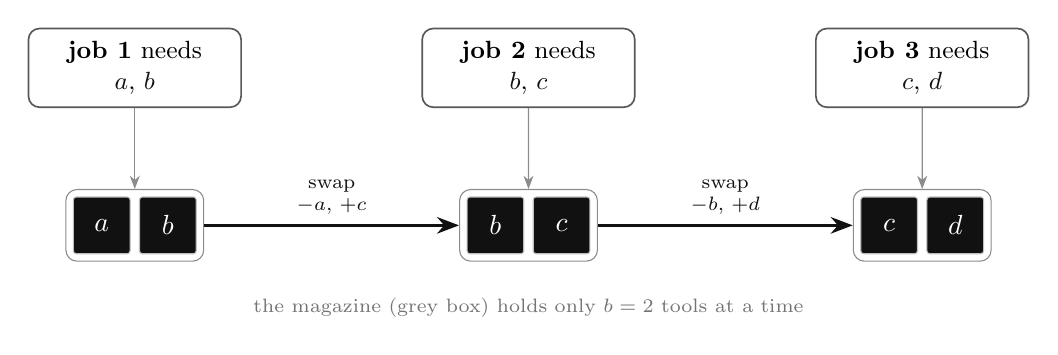
\begin{tikzpicture}[
   font=\small, >=Stealth,
   job/.style={draw=cBlue!70, fill=white, rounded corners, semithick,
               minimum width=2.7cm, minimum height=1.0cm, align=center},
   chip/.style={draw=black!25, rounded corners=1pt, minimum size=0.72cm,
                inner sep=0pt, font=\bfseries, text=white},
   swaparr/.style={->, line width=1.1pt, cRed}]
  \node[job] (j1) at (0,2)   {\textbf{job 1} needs\\ {\color{cRed}$a$}, {\color{cBlue}$b$}};
  \node[job] (j2) at (5,2)   {\textbf{job 2} needs\\ {\color{cBlue}$b$}, {\color{cGreen}$c$}};
  \node[job] (j3) at (10,2)  {\textbf{job 3} needs\\ {\color{cGreen}$c$}, {\color{cOrange}$d$}};
  \node[chip,fill=cRed]    (m1a) at (-0.42,0) {$a$};
  \node[chip,fill=cBlue]   (m1b) at ( 0.42,0) {$b$};
  \node[chip,fill=cBlue]   (m2a) at ( 4.58,0) {$b$};
  \node[chip,fill=cGreen]  (m2b) at ( 5.42,0) {$c$};
  \node[chip,fill=cGreen]  (m3a) at ( 9.58,0) {$c$};
  \node[chip,fill=cOrange] (m3b) at (10.42,0) {$d$};
  \node[draw=black!45, rounded corners, fit=(m1a)(m1b), inner sep=2.5pt] (m1) {};
  \node[draw=black!45, rounded corners, fit=(m2a)(m2b), inner sep=2.5pt] (m2) {};
  \node[draw=black!45, rounded corners, fit=(m3a)(m3b), inner sep=2.5pt] (m3) {};
  \draw[->,black!45] (j1) -- (m1);  \draw[->,black!45] (j2) -- (m2);  \draw[->,black!45] (j3) -- (m3);
  \draw[swaparr] (m1) -- (m2)
     node[midway,above,font=\scriptsize,align=center]{swap\\ $-a$, $+c$};
  \draw[swaparr] (m2) -- (m3)
     node[midway,above,font=\scriptsize,align=center]{swap\\ $-b$, $+d$};
  \node[font=\scriptsize,text=black!55] at (5,-1.05) {the magazine (grey box) holds only $b=2$ tools at a time};
\end{tikzpicture}
\caption{The problem at its smallest. Three jobs run from left to right on a
machine whose magazine holds two tools. A job can run only when both of its tools
are loaded. Filling the magazine for job~1 costs two insertions. Each later job
happens to share one tool with the job before it, so one tool is swapped in at each
step: two more insertions, four in total. Changing the order of the jobs, or making
the magazine larger, changes that count. Finding the order that minimises the total,
over all $n!$ orders, is the SSP.}
\label{fig:setup}
\end{figure}

Figure~\ref{fig:twoorders} takes that same instance and changes only the order, which
changes the count.

\begin{figure}[ht]
\centering
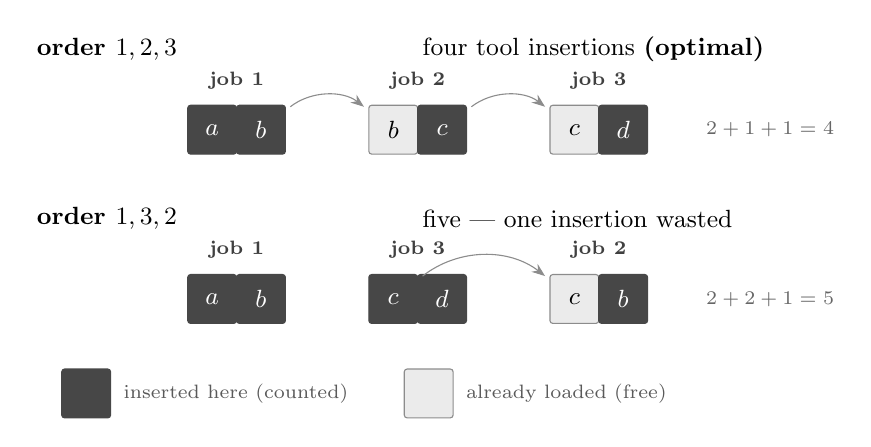
\begin{tikzpicture}[
   font=\small, >=Stealth,
   slot/.style={draw=black!45, rounded corners=1pt, minimum size=0.62cm,
                inner sep=0pt, font=\small},
   fresh/.style={slot, fill=black!72, text=white, draw=black!72},
   held/.style={slot, fill=black!8},
   jl/.style={font=\scriptsize\bfseries, text=black!75}]

 % ---------------- row 1 : order 1,2,3 -> cost 4 ----------------
 \begin{scope}
   \node[font=\small\bfseries, anchor=west] at (-2.35,1.02) {order $1,2,3$};
   \node[anchor=west, font=\small] at (2.55,1.02) {four tool insertions \textbf{(optimal)}};
   \foreach \x/\lab in {0/{job 1},2.3/{job 2},4.6/{job 3}}
     \node[jl] at (\x+0.31,0.62) {\lab};
   % job1 {a,b}: both new
   \node[fresh] (r1a) at (0,0)    {$a$};  \node[fresh] (r1b) at (0.62,0) {$b$};
   % job2 {b,c}: b held, c new
   \node[held]  (r2b) at (2.3,0)  {$b$};  \node[fresh] (r2c) at (2.92,0) {$c$};
   % job3 {c,d}: c held, d new
   \node[held]  (r3c) at (4.6,0)  {$c$};  \node[fresh] (r3d) at (5.22,0) {$d$};
   \foreach \a/\b in {r1b/r2b, r2c/r3c}
     \draw[->, black!45, shorten >=2pt, shorten <=2pt] (\a) to[bend left=38] (\b);
   \node[font=\scriptsize, text=black!60, anchor=west] at (6.15,0) {$2+1+1=4$};
 \end{scope}

 % ---------------- row 2 : order 1,3,2 -> cost 5 ----------------
 \begin{scope}[yshift=-2.15cm]
   \node[font=\small\bfseries, anchor=west] at (-2.35,1.02) {order $1,3,2$};
   \node[anchor=west, font=\small] at (2.55,1.02) {five --- one insertion wasted};
   \foreach \x/\lab in {0/{job 1},2.3/{job 3},4.6/{job 2}}
     \node[jl] at (\x+0.31,0.62) {\lab};
   \node[fresh] (s1a) at (0,0)    {$a$};  \node[fresh] (s1b) at (0.62,0) {$b$};
   \node[fresh] (s2c) at (2.3,0)  {$c$};  \node[fresh] (s2d) at (2.92,0) {$d$};
   \node[held]  (s3c) at (4.6,0)  {$c$};  \node[fresh] (s3b) at (5.22,0) {$b$};
   \draw[->, black!45, shorten >=2pt, shorten <=2pt] (s2c) to[bend left=38] (s3c);
   \node[font=\scriptsize, text=black!60, anchor=west] at (6.15,0) {$2+2+1=5$};
 \end{scope}

 % ---------------- legend ----------------
 \node[fresh] (lg1) at (-1.6,-3.35) {};
 \node[anchor=west, font=\scriptsize, text=black!65] at (-1.25,-3.35) {inserted here (counted)};
 \node[held]  (lg2) at (2.75,-3.35) {};
 \node[anchor=west, font=\scriptsize, text=black!65] at (3.1,-3.35) {already loaded (free)};
\end{tikzpicture}
\caption{The same three jobs, two orders. Running job~2 between jobs~1 and~3 lets the
magazine hand tool~$b$ forward and then tool~$c$ forward, so only one tool is fetched at
each step. Running job~3 second breaks both chains: the magazine must be emptied and
refilled, and tool~$b$ --- discarded after job~1 --- has to be fetched a second time.
That repeat is the only difference between the two rows, and it is what an exact method
has to reason about. There are $n!$ orders and no way to see which chains survive
without searching.}
\label{fig:twoorders}
\end{figure}

Figure~\ref{fig:landscape} does the same on a real benchmark instance of eight jobs,
small enough that all $40{,}320$ orders can be enumerated. It shows how much lies
between a good order and a bad one, and where the bound that every exact method starts
from sits relative to both.

\begin{figure}[ht]\centering
\begin{tikzpicture}
\begin{axis}[reportaxis, height=5.9cm,
  ybar, bar width=8.5pt,
  xlabel={tool switches required by an ordering},
  ylabel={number of orderings},
  xmin=8.6, xmax=25, ymin=0, ymax=10600,
  xtick={10,13,14,16,18,20,22,24},
  ytick={0,2000,4000,6000,8000},
  scaled y ticks=false,
  yticklabel style={/pgf/number format/fixed,
                    /pgf/number format/1000 sep={,}},
  clip=false]
  \addplot[draw=black!65, fill=black!22] table[x=cost,y=count] {figdata/landscape.dat};
  % the coverage bound: below everything achievable
  \draw[black, line width=1pt, dashed] (axis cs:10,0) -- (axis cs:10,9700);
  \node[anchor=west, font=\scriptsize, align=left] at (axis cs:10.25,9100)
    {\textbf{coverage bound $q=10$}\\[-1pt] what every compact\\[-1pt] relaxation returns};
  % the optimum
  \draw[black, line width=1pt] (axis cs:13,0) -- (axis cs:13,6100);
  \node[anchor=north east, font=\scriptsize, align=right] at (axis cs:12.7,6100)
    {\textbf{optimum $\Zst=13$}\\[-1pt] reached by $180$\\[-1pt] of the $40{,}320$};
  % the median ordering
  \draw[black!55, line width=0.8pt, densely dotted] (axis cs:18,0) -- (axis cs:18,9700);
  \node[anchor=west, font=\scriptsize, text=black!60, align=left] at (axis cs:18.3,9250)
    {median ordering: $18$};
\end{axis}
\end{tikzpicture}
\caption{Every one of the $40{,}320$ orderings of instance \texttt{L1-1}
($n=8$ jobs, $\lvert\U\rvert=15$ tools, magazine $b=5$), enumerated, and the tool
switches each requires. Three things are visible at once. A randomly chosen ordering
costs $18$, and the best costs $13$, so the choice of order is worth about a third of
the total. Only $180$ orderings out of forty thousand are optimal, which is why the
outer problem is hard. And the counting bound of $q=10$, which is what the SSPMF
compact baseline returns, lies \emph{below the entire
distribution}: no ordering whatsoever attains it. A solver given that bound cannot
prove any ordering optimal until it has closed a gap of three by branching alone.
Section~\ref{sec:comp} shows what that costs in practice and Section~\ref{sec:disc} why
the bound behaves this way.}
\label{fig:landscape}
\end{figure}

The same structure appears well outside machining, and everything in this report
carries over. In printed-circuit-board assembly the tools are component feeders and
the jobs are the boards. In colour printing they are ink cartridges on a press, and
the problem occurs there in exactly the form studied here
\citep{Burger2015}. In warehouse picking they are the items a picker can carry at
once. What matters in each case is that a limited, reusable resource serves groups
of demands, and that the order of the demands can be chosen.

\subsection{Why the problem is hard, and why it is still open}\label{ssec:intro-why}

The two decisions behave very differently.

Loading is easy. Once the order of the jobs is fixed, the cheapest loading policy is
known in closed form. It is the Keep Tool Needed Soonest rule of \citet{Tang1988}:
when a tool must be inserted into a full magazine, remove the tool whose next use
lies furthest in the future. The rule is optimal, and it runs in
$O(n\lvert T\rvert)$ time.

Ordering is hard. \citet{Crama1994} proved the SSP NP-hard for every fixed magazine
capacity $b\ge2$. The difficulty is that a good order places jobs with similar tool
requirements next to one another, but ``similar'' here means nothing more than
overlapping sets, with no natural distance to measure it, and the magazine limit
couples jobs that are far apart in the order.

That combination --- an easy inner problem inside a hard outer one --- is exactly
what decomposition methods are built for, and it is the reason the SSP has attracted
exact methods for four decades. Two gaps in that literature motivate this work.

The first is on the practical side. Exact methods for the integrated SSP exist and
are used as baselines in Section~\ref{sec:comp}, but practice does not generally rely on
them. The standard
approach groups the jobs into as few magazine-fitting batches as possible, then
orders the batches. It is fast, and where it has been measured against exact optima in
industrial printing it does well \citep{Burger2015}. The leading hybrid genetic search
instead starts from random job orders improved by local search \citep{Mecler2021}; it
does not use grouping solutions as seeds. \citet{CramaKlundert1999} analyse the
group-then-sequence construction and prove
that it is a $b$-approximation. What has not been done is to sharpen that ratio, to say
on which instances the method is exact, or to distinguish the two different values the
method can be read as returning --- and the third of these turns out to change the first
two. How far
from optimal it can be, and on which instances it is exact, are open questions.

The second is on the exact side. The three compact integer formulations reimplemented
as campaign baselines have weak linear relaxations, and the strongest of that baseline
set, SSPMF \citep{daSilva2024}, relaxes exactly to the number of tools minus the
magazine capacity, under its assumption that every tool is used. That is an
elementary counting bound: every tool that does not fit in the initial magazine must be
inserted at some point. Thus the best relaxation among the three reimplemented
baselines is this counting argument, and a solver relying on it cannot prove optimality
where the bound is loose. This is deliberately not a literature-wide ranking:
the symmetry-strengthened JGSMF model of \citet{Akhundov2024}, for example, was not
implemented in this internship.

\subsection{What was done during this internship}\label{ssec:intro-done}

The internship took place at the Laboratoire d'Informatique, de Mod\'elisation et
d'Optimisation des Syst\`emes (LIMOS), under the advisorship of Prof.~Rafael
Colares and Prof.~Annegret Wagler, with Dr.~Renaud Chicoisne as academic
supervisor. The research directions were set by the advisors, and this report is
organised around them. They are recorded here explicitly, so that the origin of
each line of work is clear.

\begin{itemize}[topsep=4pt,itemsep=3pt]
  \item \textbf{The configuration-based view of the problem} was proposed by
  Prof.~Colares and Prof.~Wagler, and frames the whole project. A
  \emph{configuration} is a full magazine, and a schedule is a walk through
  configurations that serves every job. Section~\ref{ssec:gtsp} develops it.

  \item \textbf{The reduction of the SSP to a generalised travelling-salesman
  problem} was set by Prof.~Colares. It is the formal content of that view, and it
  is what makes both exact methods below natural.

  \item \textbf{The analysis of the gap between the two-phase heuristic and the
  optimum} was set by Prof.~Wagler, together with the request to enumerate the
  integral solutions of the grouping problem with PORTA. Her specific questions
  were to construct worst-case examples with the number of groups fixed, to study
  instances where the gap is attained, and to prove an upper bound tighter than the
  trivial $b(\Kst-1)$. Section~\ref{sec:gap} answers the first two and gives
  several answers to the third.

  \item \textbf{The study of the grouping problem through clutters and blocking
  duality} was also set by Prof.~Wagler. Section~\ref{ssec:clutter} reports it.

  \item \textbf{The branch-and-Benders-cut algorithm} was proposed by
  Prof.~Colares, following the internship report of \citet{Kashou2025}, which
  applies the same architecture to a production-line balancing problem. The
  suggestion was to try lazy cuts first and cuts at fractional solutions second.
  Section~\ref{ssec:bbc} develops it and Section~\ref{ssec:results-bbc} measures it.

  \item \textbf{The position-indexed formulations} were proposed by
  Prof.~Colares, including the idea that makes them work: fixing a row set that
  is polynomial in the instance size, so that column generation only ever adds
  columns to rows that already exist. The purpose was to make branch-and-price over
  configurations possible. Section~\ref{ssec:pos} develops them.
\end{itemize}

\noindent
Work on these directions fell into three parts, and each has a section of its own
below.

The first was theoretical: the structural analysis of Section~\ref{sec:gap}. It
answers the questions Prof.~Wagler set, and raises several that emerged from them.

The second was implementation. The branch-and-Benders-cut solver, the two
branch-and-price prototypes, three formulations from the literature reimplemented as
baselines, a hybrid genetic heuristic, the campaign harness and the cluster pipeline
were built and validated against brute-force optima before any of them was used to
produce a result. Section~\ref{sec:exact} describes the methods and
Appendix~\ref{app:repro} the code.

The third was experimental: the benchmark campaign of Section~\ref{sec:comp}, run on
the LIMOS cluster over the standard instance families under a uniform protocol,
together with the small-scale enumeration used throughout Section~\ref{sec:gap} to
test each statement as it was made. One correction made during the campaign is worth
recording, because it changed the results substantially: the Benders master was found
to be missing the tool coverage bound, and the campaign was re-run once it was added.

\subsection{Conventions}\label{ssec:intro-read}

Section~\ref{sec:prelim} defines the problem and everything used to attack it,
including a self-contained account of the integer-programming background in
Section~\ref{ssec:toolkit}, which a reader who already knows integer programming may
skip. Section~\ref{sec:sota} reviews the literature. Longer proofs are in
Appendix~\ref{app:proofs}, the verification program in Appendix~\ref{app:verify}, and
Appendix~\ref{app:repro} says how to reproduce every experiment.

Every formal result carries a label --- Theorem, Proposition, Lemma, Corollary,
Observation, or Conjecture --- and the labels are used strictly. A Proposition has a
proof. An Observation was established by running a program. A Conjecture has neither,
only evidence. Where an argument is given but has not been independently checked it is
headed \emph{Supporting argument} rather than \emph{Proof}. The distinction is kept
even where it makes the text less confident.

%==============================================================================
\section{The problem and the tools used to attack it}\label{sec:prelim}
%==============================================================================

This section defines the SSP, the rule that solves its inner problem, the
grouping view that the whole report is built on, and the two elementary lower
bounds that everything later is measured against. It ends with a self-contained
account of the integer-programming background used in Section~\ref{sec:exact}.

\subsection{The Job Sequencing and Tool Switching Problem}\label{ssec:ssp}

An instance consists of $n$ jobs $J=\rset{1,\dots,n}$, a set of tools $T$, a
magazine capacity $b\in\mathbb{N}$, and for each job $j$ a set of required tools
$T_j\subseteq T$ with $1\le\lvert T_j\rvert\le b$. The requirement
$\lvert T_j\rvert\le b$ is necessary: a job needing more tools than the magazine
holds could never be run. Write $\U=\bigcup_{j\in J}T_j$ for the set of tools that
some job requires. Tools outside $\U$ play no part and are ignored.
If $b>\lvert\U\rvert$, replacing $b$ by $\lvert\U\rvert$ changes no feasible
schedule or insertion cost. We make that preprocessing convention once and henceforth
assume $b\le\lvert\U\rvert$; in particular $q=\lvert\U\rvert-b$ is non-negative.

\begin{definition}[Schedule and switch cost]\label{def:ssp}
A \emph{schedule} is a pair $(\pi,\mathbf{M})$, where $\pi$ is a permutation of $J$
giving the order in which the jobs run, and $\mathbf{M}=(M_1,\dots,M_n)$ gives the
magazine contents at each position. It is feasible when
\[
  \lvert M_i\rvert\le b \quad\text{and}\quad T_{\pi(i)}\subseteq M_i
  \qquad (i=1,\dots,n),
\]
that is, when the magazine never overflows and always holds what the current job
  needs. With $M_0=\varnothing$, its \emph{empty-start cost} is
\[
  \sum_{i=1}^{n}\lvert M_i\setminus M_{i-1}\rvert .
\]
The \emph{free-initial cost} omits the $i=1$ term: the first fill is free and every
later insertion is charged. Throughout the theory $\Zst$ denotes the minimum
free-initial cost; $\Zempty$ denotes the minimum empty-start cost reported by the
computational study.
\end{definition}

Counting insertions rather than removals is the standard cost model. Under a fixed
capacity each insertion into a full magazine forces exactly one removal, so the two
counts differ only at the start of the schedule. Section~\ref{ssec:conv} makes that
difference precise.

The following instance is used as an example throughout the report.

\begin{example}[The $6$-ring]\label{ex:ring}
The \emph{$6$-ring} has six jobs, six tools and capacity $b=3$. Job $j$ requires
$T_j=\rset{j,\,j+1}$, with indices taken modulo $6$, so that $T_6=\rset{6,1}$.
Consecutive jobs share exactly one tool and non-consecutive jobs share none. Its
job--tool incidence matrix, with rows for tools and columns for jobs and a blank
denoting $0$, is
\[
\begin{array}{c|cccccc}
      & 1 & 2 & 3 & 4 & 5 & 6\\\hline
 t_1  & 1 &   &   &   &   & 1\\
 t_2  & 1 & 1 &   &   &   &  \\
 t_3  &   & 1 & 1 &   &   &  \\
 t_4  &   &   & 1 & 1 &   &  \\
 t_5  &   &   &   & 1 & 1 &  \\
 t_6  &   &   &   &   & 1 & 1
\end{array}
\]
Figure~\ref{fig:ring} draws it. Its optima are $\Zempty=6$ empty-start and
$\Zst=3$ free-initial; Section~\ref{ssec:ktns} computes them.
\end{example}

\begin{figure}[h]\centering
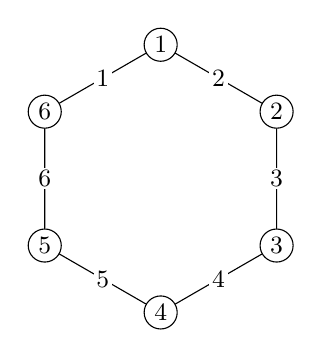
\begin{tikzpicture}[scale=1.7,line cap=round,every node/.style={font=\small}]
  \foreach \i in {1,...,6}{
    \node[draw,circle,fill=white,inner sep=1.6pt] (j\i) at ({90-(\i-1)*60}:1) {$\i$};
  }
  \foreach \a/\b/\t in {1/2/2,2/3/3,3/4/4,4/5/5,5/6/6,6/1/1}{
    \draw (j\a)--(j\b) node[midway,fill=white,inner sep=1pt]{$\t$};
  }
\end{tikzpicture}
\caption{The $6$-ring. The six jobs lie on a cycle. Each edge is labelled by the
single tool its two endpoint jobs share, so job $j$ requires the two tools on the
edges meeting it. Adjacent jobs overlap in one tool; non-adjacent jobs are
tool-disjoint.}\label{fig:ring}
\end{figure}

\subsection{Loading tools for a fixed order}\label{ssec:ktns}

Suppose the order of the jobs is already decided. What remains is to choose the
magazine contents at each position. This inner problem has a closed-form solution.

\begin{proposition}[\citealp{Tang1988}]\label{prop:ktns}
Fix a permutation $\pi$. The following rule produces a magazine sequence of minimum
switch cost. Process the jobs in the order $\pi$. Whenever a required tool is
absent, insert it; if the magazine is full, first remove a tool whose next required
use lies furthest in the future, removing a tool never required again if one
exists. This is the \emph{Keep Tool Needed Soonest} (KTNS) rule. It runs in
$O(n\lvert T\rvert)$ time, and no loading policy for $\pi$ costs less.
\end{proposition}

The proof is in \citet{Tang1988}; \citet{Crama1994} give a second proof through
interval matrices. Write $\KTNS(\pi)$ for its free-initial value (subtracting the
constant first fill from the empty-start count). Since the rule is optimal for every
fixed order,
\[
  \Zst \;=\; \min_{\pi}\ \KTNS(\pi),
\]
so the SSP reduces to a pure sequencing problem. Every method in this report is
some way of searching over orders while delegating the loading to this rule.

\begin{example}[KTNS on the $6$-ring]\label{ex:ktns}
Take the $6$-ring and the cyclic order $1,2,3,4,5,6$. Figure~\ref{fig:ktns} traces
it. The magazine starts empty and holds three tools.

Jobs~1 and~2 need $\rset{1,2}$ and $\rset{2,3}$, so the first magazine is filled
with $\rset{1,2,3}$: three insertions, and this serves both jobs. At position~3,
job~3 needs $\rset{3,4}$. Tool~3 is already loaded, so only tool~4 is inserted, and
one resident tool must leave. This is where the rule does its work. Of the residents
$\rset{1,2,3}$, tool~2 is never required again, while tool~1 is required by job~6 at
the very end. The rule removes tool~2 and keeps tool~1. Positions~4 and~5 repeat the
pattern, inserting one new tool and removing the one whose next use is furthest
away. Position~6 needs $\rset{6,1}$, and both are present, so it is free.

The total is three insertions to fill the magazine plus one at each of positions
$3,4,5$: six insertions, or three once the first fill is not charged. Keeping tool~1
loaded through three positions where it is not used is what the rule buys. A policy
that removed tool~1 at position~3 would have to reload it at position~6 and would
pay seven.
\end{example}

\begin{figure}[t]\centering
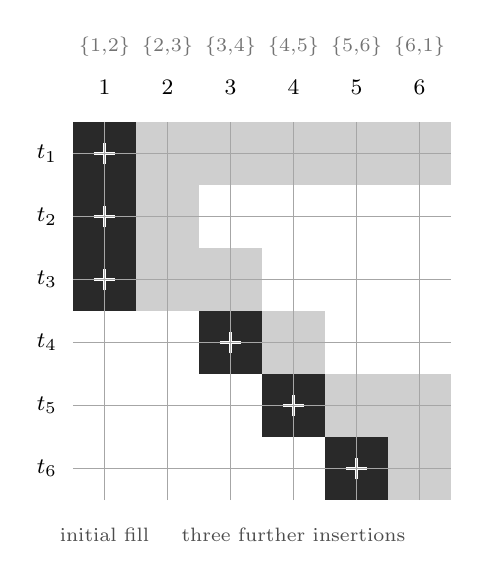
\begin{tikzpicture}[x=0.8cm,y=0.8cm,font=\footnotesize]
  \foreach \p/\req in {1/{1{,}2},2/{2{,}3},3/{3{,}4},4/{4{,}5},5/{5{,}6},6/{6{,}1}}{
    \node[font=\footnotesize] at (\p,6.05) {\p};
    \node[font=\scriptsize,text=black!55] at (\p,6.7) {$\{\req\}$};}
  \foreach \t/\y in {1/5,2/4,3/3,4/2,5/1,6/0}{\node[anchor=east,font=\footnotesize] at (0.4,\y) {$t_{\t}$};}
  \foreach \p/\y in {2/5,3/5,4/5,5/5,6/5, 2/4, 2/3,3/3, 4/2, 5/1,6/1, 6/0}{
     \fill[cBlue!20] (\p-0.5,\y-0.5) rectangle (\p+0.5,\y+0.5);}
  \foreach \p/\y in {1/5,1/4,1/3, 3/2, 4/1, 5/0}{
     \fill[cOrange!90] (\p-0.5,\y-0.5) rectangle (\p+0.5,\y+0.5);
     \draw[white,line width=0.9pt] (\p-0.17,\y)--(\p+0.17,\y);
     \draw[white,line width=0.9pt] (\p,\y-0.17)--(\p,\y+0.17);}
  \draw[black!35,step=1] (0.5,-0.5) grid (6.5,5.5);
  \node[font=\scriptsize,text=black!70] at (1,-1.05) {initial fill};
  \node[font=\scriptsize,text=black!70] at (4,-1.05) {three further insertions};
\end{tikzpicture}
\caption{KTNS on the $6$-ring in the order $1,2,3,4,5,6$. Columns are the six
processing positions, with the tools each job needs written above them; rows are the
six tools. A shaded cell means the tool sits in the magazine at that position; a
``$+$'' marks an insertion. Every column holds exactly three tools. Tool~1, in the
top row, is loaded once and kept across all six positions, idle in the middle, so
that it need not be reloaded for job~6. The cost is three insertions to fill the
magazine and three afterwards: six in the empty-start cost, three in the
free-initial cost.}
\label{fig:ktns}
\end{figure}

\begin{remark}[The loading problem is offline caching]\label{rem:belady}
For a fixed order the loading problem is exactly offline paging. The magazine is a
cache of size $b$, position $i$ requests the set $T_{\pi(i)}$, and an insertion is a
cache miss. Proposition~\ref{prop:ktns} is then the tool-switching form of
B\'el\'ady's optimal replacement rule, which removes the item whose next request is
furthest in the future and which minimises misses on any fixed request sequence
\citep{Belady1966}. The comparison is informative. Paging takes the request order as
given; the SSP may reorder the jobs, and it is that freedom which turns a
polynomially solvable caching problem into an NP-hard one.
\end{remark}

\subsection{Configurations}\label{ssec:gtsp}

The magazine, not the job, is the natural unit for what follows.

\begin{definition}[Configuration, cluster, transition cost]\label{def:config}
A \emph{configuration} is a set $C\subseteq\U$ with exactly $\lvert C\rvert=b$
tools. The set of all configurations is written $\confs$. For a job $j$, the
\emph{cluster} $H_j=\rset{C\in\confs : T_j\subseteq C}$ is the set of
configurations able to serve $j$. For two configurations, the \emph{transition
cost} is the number of tools that must be inserted to pass from one to the other,
\[
  d(C,C') \;=\; \lvert C'\setminus C\rvert .
\]
\end{definition}

Restricting attention to full magazines costs nothing. Keeping a tool that might be
useful later never increases the number of insertions, so some optimal schedule
keeps the magazine full at every position whenever $\lvert\U\rvert\ge b$.

Under this view a schedule is a walk $C_{(1)},\dots,C_{(r)}$ through $\confs$ that
visits at least one configuration of every cluster $H_j$, and its cost is
$\sum_l d(C_{(l)},C_{(l+1)})$. That a schedule and such a walk have equal cost is
immediate in one direction: take any schedule, delete repetitions from its sequence
of magazines, and what remains is a walk of the same cost that serves every job. The
converse is Theorem~\ref{thm:grouping} in Section~\ref{ssec:exact}.

The SSP is therefore a generalised travelling-salesman problem over $\confs$, in
which the clusters \emph{overlap}: one configuration can serve many jobs. The
formulation is documented by \citet{Moreira2026}, who attributes it to a 2024 personal
communication by Rafael Colares, Mauricio de Souza and Annegret Wagler. The overlap is what separates it
from the textbook generalised travelling-salesman problem with disjoint clusters
\citep{Noon1993,Fischetti1997,Pop2024}, and it is why the standard reductions for
that problem do not transfer.

\subsection{Grouping the jobs}\label{ssec:jgp}

Section~\ref{ssec:ktns} settled the loading problem, so what remains is the order.
Solving for the order directly is hard, so practice does something indirect. It
first asks a simpler question: which jobs could share a magazine?

\begin{definition}[Feasible group]\label{def:group}
A set of jobs $G\subseteq J$ is a \emph{feasible group} if the tools its jobs need,
taken together, fit in the magazine:
\[
  \Bigl\lvert \bigcup_{j\in G} T_j \Bigr\rvert \;\le\; b .
\]
\end{definition}

A feasible group can be run from start to finish without a single tool change. Load
the tools its jobs need, run them in any order, and only then change anything. This
makes the following question natural.

\begin{definition}[Job Grouping Problem]\label{def:jgp}
The \emph{Job Grouping Problem} (JGP) is the problem of partitioning $J$ into as few
feasible groups as possible. The smallest possible number of groups is written
$\Kst$.
\end{definition}

The JGP ignores order completely. It asks only how the jobs may be divided. It is
itself NP-hard, but it is far easier in practice than the SSP, and it is solved
exactly on every instance size considered here, by the asymmetric-representatives
formulation of \citet{Jans2013} or by the set-covering column generation of
\citet{Crama1994Column}.

Two problems now sit next to each other. The JGP says which jobs may share a
magazine. The SSP asks for an order. The standard heuristic joins them, in three
steps.

\begin{enumerate}[topsep=4pt,itemsep=2pt]
  \item \textbf{Group.} Solve the JGP. This returns $\Kst$ feasible groups
  $G_1,\dots,G_{\Kst}$, and for each group a configuration $C_l$ containing
  everything that group needs.
  \item \textbf{Sequence.} Decide the order of the groups. Moving from
  configuration $C$ to configuration $C'$ costs $d(C,C')$, so finding the cheapest
  order of the $\Kst$ configurations is a travelling-salesman problem on $\Kst$
  points, which is small enough to solve exactly
  \citep{Applegate2006,Helsgaun2015}.
  \item \textbf{Evaluate.} Write out the jobs group by group, in the order chosen in
  step~2, to obtain a single job order. Apply KTNS to that order and report its cost.
\end{enumerate}

This is the method studied throughout this report. It is fast, it is what
practitioners use, and its output is always a feasible schedule, so its cost is never
below $\Zst$.

\begin{example}[The heuristic on the $6$-ring]\label{ex:jgp-ring}
Step~1 returns $\Kst=3$ for the $6$-ring. One optimal grouping is
\[
  G_1=\rset{1,2},\qquad G_2=\rset{3,4},\qquad G_3=\rset{5,6},
\]
whose tool requirements are $\rset{1,2,3}$, $\rset{3,4,5}$ and $\rset{5,6,1}$. Each
has exactly three tools, so each group fixes its configuration with no freedom left:
$C_1=\rset{1,2,3}$, $C_2=\rset{3,4,5}$, $C_3=\rset{5,6,1}$.

Step~2 compares them. Any two share exactly one tool, so moving between any two
costs two insertions. Every order of the three groups costs the same, and step~2 may
return any of them. Take $G_1,G_2,G_3$.

Step~3 writes out the jobs group by group, giving the order $1,2,3,4,5,6$, and
applies KTNS. That is the order traced in Example~\ref{ex:ktns}, and its cost is six
insertions, or three once the first fill is not charged.
\end{example}

Two features of this example matter later.

First, the method does not fully determine its own answer. Step~1 may return several
optimal groupings, step~2 may face ties as it does here, and the order of the jobs
\emph{inside} a group is left open by all three steps. Different choices can give
different costs. Throughout this report the heuristic is read in its most favourable
form: its cost is the best value reachable over all of these choices. This is the
reading that makes a comparison with $\Zst$ meaningful, because any weaker reading
would measure the tie-breaking rule rather than the method.

Second, and less obviously, step~3 does something that step~2 did not anticipate.
That is the subject of the next subsection.

\subsection{Two ways to measure the heuristic}\label{ssec:frames}

Steps~1 and~2 reason entirely in terms of configurations. Each group is assigned one
magazine, and that magazine is imagined to stay loaded while the whole group runs.
Under that picture a schedule is a walk through $\Kst$ configurations, and its cost
is the sum of the transition costs along the walk.

Step~3 does not do this. It discards the configurations, keeps only the job order
they produced, and hands that order to KTNS. KTNS may change the magazine between
any two consecutive jobs, including two jobs of the same group. The group structure
survives only as an ordering of the jobs; it does not constrain the magazine.

The two readings give different numbers. Both appear in the literature without being
distinguished. This report separates them.

\begin{definition}[The walk value and the heuristic value]\label{def:frames}
Let $\mathcal{P}$ range over the partitions of $J$ into $\Kst$ feasible groups. For
each such partition let the configurations be chosen and ordered as cheaply as
possible, and write
\[
  \Hwalk
  \;=\;\min_{\mathcal{P}}\;\min_{\sigma}\;
        \sum_{l=1}^{\Kst-1} d\bigl(C_{\sigma(l)},C_{\sigma(l+1)}\bigr)
\]
for the cheapest such walk. Write $H$ for the cost of the two-phase heuristic as
defined in Section~\ref{ssec:jgp}: the minimum, over the same partitions, over all
orders of the groups and all orders of the jobs within each group, of the KTNS cost
of the resulting job order.
\end{definition}

\begin{remark}[$H$ is an envelope, not the output of an implementation]\label{rem:envelope}
Both $\Hwalk$ and $H$ minimise over every choice the method leaves open: which
minimum-cardinality grouping, which order of the groups, and which order of the jobs
inside each group. They are therefore the \emph{best} value reachable by the two-phase
construction, not the value a particular implementation returns. Any implementation
resolves those choices by some rule and returns a value at least as large, so a bound
proved here for $H$ bounds the best case of the construction and is not by itself an
approximation guarantee for a deterministic implementation of it. The choice is
deliberate --- the alternative measures a tie-breaking rule rather than the method ---
but every gap statement in Section~\ref{sec:gap} should be read with it in mind.
\end{remark}

\begin{proposition}\label{prop:frames}
For every instance, $H\le\Hwalk$.
\end{proposition}

\begin{proof}
Fix a partition and an order of its groups attaining $\Hwalk$. Writing the jobs out
group by group in that order gives a job order. Holding each group's configuration
fixed while its jobs run is one admissible loading for that order, and its cost is
exactly the walk cost. By Proposition~\ref{prop:ktns}, KTNS returns the cheapest
loading for that order, so the KTNS cost is at most the walk cost. Since $H$
minimises over at least this one job order, $H\le\Hwalk$.
\end{proof}

The inequality can be strict, and it is strict on the running example.

\begin{example}[The two values differ on the $6$-ring]\label{ex:frames-ring}
Continue Example~\ref{ex:jgp-ring}. The walk pays three insertions to build
$C_1=\rset{1,2,3}$, then two to reach $C_2=\rset{3,4,5}$, then two to reach
$C_3=\rset{5,6,1}$. That is $\Hwalk=7$, or $4$ free-initial. KTNS on the same job
order costs $6$, or $3$ free-initial. Since $\Zst=3$ free-initial, the heuristic is
\emph{optimal} on the $6$-ring while the walk value is one above the optimum.

Figure~\ref{fig:frames} shows where the two part company. The walk requires the
middle group to run under $C_2=\rset{3,4,5}$ and nothing else. Tool~1 is not in
$C_2$, so it is removed at position~3 and must be reloaded at position~5 for job~6.
KTNS is not bound to $C_2$. It holds $\rset{1,3,4}$ at position~3 and
$\rset{1,4,5}$ at position~4, two different magazines inside one group, each
serving its own job, and so keeps tool~1 loaded throughout. The one re-insertion is
avoided.
\end{example}

\begin{figure}[t]\centering
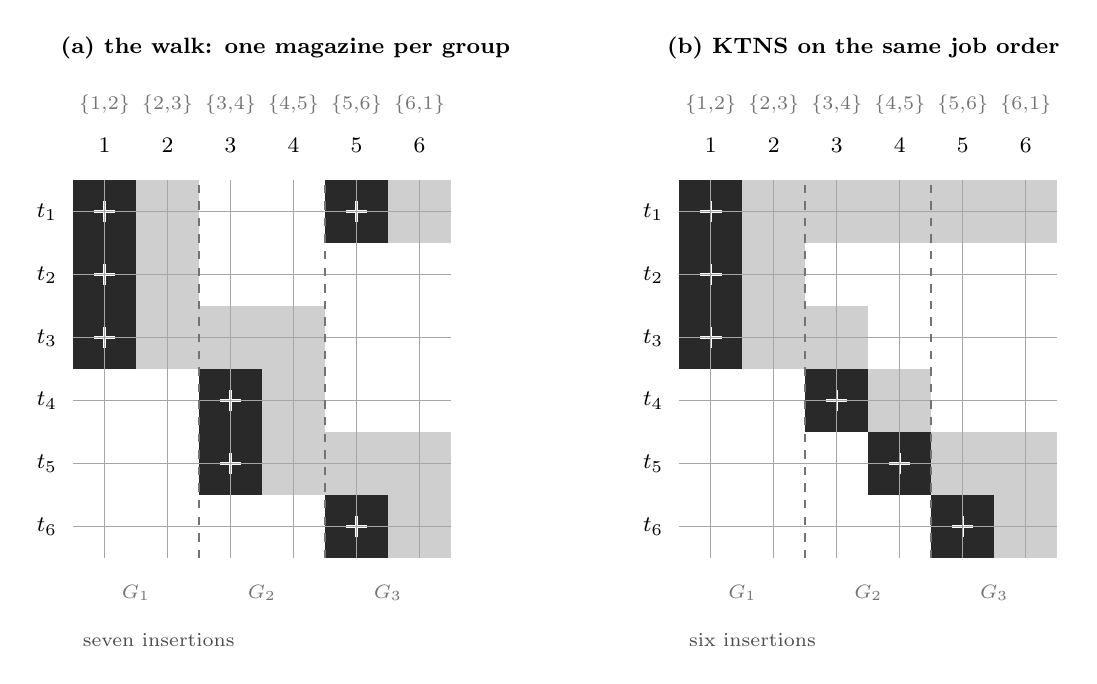
\begin{tikzpicture}[x=0.8cm,y=0.8cm,font=\footnotesize]
 % ---------------- (a) the configuration walk ----------------
 \begin{scope}
  \node[font=\footnotesize\bfseries,anchor=west] at (0.15,7.6)
     {(a) the walk: one magazine per group};
  \foreach \p/\req in {1/{1{,}2},2/{2{,}3},3/{3{,}4},4/{4{,}5},5/{5{,}6},6/{6{,}1}}{
    \node[font=\footnotesize] at (\p,6.05) {\p};
    \node[font=\scriptsize,text=black!55] at (\p,6.7) {$\{\req\}$};}
  \foreach \t/\y in {1/5,2/4,3/3,4/2,5/1,6/0}{
    \node[anchor=east,font=\footnotesize] at (0.4,\y) {$t_{\t}$};}
  \foreach \p/\y in {1/5,2/5,5/5,6/5, 1/4,2/4, 1/3,2/3,3/3,4/3,
                     3/2,4/2, 3/1,4/1,5/1,6/1, 5/0,6/0}{
     \fill[cBlue!20] (\p-0.5,\y-0.5) rectangle (\p+0.5,\y+0.5);}
  \foreach \p/\y in {1/5,1/4,1/3, 3/2,3/1, 5/5,5/0}{
     \fill[cOrange!90] (\p-0.5,\y-0.5) rectangle (\p+0.5,\y+0.5);
     \draw[white,line width=0.9pt] (\p-0.17,\y)--(\p+0.17,\y);
     \draw[white,line width=0.9pt] (\p,\y-0.17)--(\p,\y+0.17);}
  \draw[black!35,step=1] (0.5,-0.5) grid (6.5,5.5);
  \draw[black!55,semithick,dashed] (2.5,-0.5) -- (2.5,5.5);
  \draw[black!55,semithick,dashed] (4.5,-0.5) -- (4.5,5.5);
  \foreach \x/\g in {1.5/1,3.5/2,5.5/3}{
    \node[font=\scriptsize,text=black!55] at (\x,-1.05) {$G_{\g}$};}
  \node[font=\scriptsize,text=black!70,anchor=west] at (0.5,-1.8)
     {seven insertions};
 \end{scope}
 % ---------------- (b) KTNS on the same job order ----------------
 \begin{scope}[xshift=7.7cm]
  \node[font=\footnotesize\bfseries,anchor=west] at (0.15,7.6)
     {(b) KTNS on the same job order};
  \foreach \p/\req in {1/{1{,}2},2/{2{,}3},3/{3{,}4},4/{4{,}5},5/{5{,}6},6/{6{,}1}}{
    \node[font=\footnotesize] at (\p,6.05) {\p};
    \node[font=\scriptsize,text=black!55] at (\p,6.7) {$\{\req\}$};}
  \foreach \t/\y in {1/5,2/4,3/3,4/2,5/1,6/0}{
    \node[anchor=east,font=\footnotesize] at (0.4,\y) {$t_{\t}$};}
  \foreach \p/\y in {1/5,2/5,3/5,4/5,5/5,6/5, 1/4,2/4, 1/3,2/3,3/3,
                     3/2,4/2, 4/1,5/1,6/1, 5/0,6/0}{
     \fill[cBlue!20] (\p-0.5,\y-0.5) rectangle (\p+0.5,\y+0.5);}
  \foreach \p/\y in {1/5,1/4,1/3, 3/2, 4/1, 5/0}{
     \fill[cOrange!90] (\p-0.5,\y-0.5) rectangle (\p+0.5,\y+0.5);
     \draw[white,line width=0.9pt] (\p-0.17,\y)--(\p+0.17,\y);
     \draw[white,line width=0.9pt] (\p,\y-0.17)--(\p,\y+0.17);}
  \draw[black!35,step=1] (0.5,-0.5) grid (6.5,5.5);
  \draw[black!55,semithick,dashed] (2.5,-0.5) -- (2.5,5.5);
  \draw[black!55,semithick,dashed] (4.5,-0.5) -- (4.5,5.5);
  \foreach \x/\g in {1.5/1,3.5/2,5.5/3}{
    \node[font=\scriptsize,text=black!55] at (\x,-1.05) {$G_{\g}$};}
  \node[font=\scriptsize,text=black!70,anchor=west] at (0.5,-1.8)
     {six insertions};
 \end{scope}
\end{tikzpicture}
\caption{The same grouping of the $6$-ring, measured two ways. Columns are the six
processing positions, with the tools each job needs above them; rows are the six
tools. A shaded cell means the tool sits in the magazine at that position; a
``$+$'' marks an insertion. The dashed lines separate the three groups. In (a) each
group runs under one fixed magazine, so tool~1, in the top row, is removed at
position~3 and reloaded at position~5 for job~6: seven insertions. In (b) KTNS may
change the magazine inside a group, so tool~1 is loaded once and kept across all six
positions, and the count is six. That single re-insertion is the whole difference
between $\Hwalk$ and $H$.}
\label{fig:frames}
\end{figure}

\begin{remark}[Why the distinction is kept throughout]\label{rem:frames}
It would be simpler to work with $\Hwalk$ alone. It has a clean description, a
shortest walk through $\Kst$ configurations, and the structural results of
Section~\ref{sec:gap} are naturally proved about it.

That simplification is not available, for two reasons. The first is that $\Hwalk$ is
not what the method returns. A practitioner running the three steps of
Section~\ref{ssec:jgp} obtains $H$, so any statement about how far the method can be
from optimal must be a statement about $H$. The second is that the two differ on
exactly the instances most often used as examples, as Example~\ref{ex:frames-ring}
shows.

Every result in Section~\ref{sec:gap} therefore names the value it is about.
Proposition~\ref{prop:frames} carries upper bounds in one direction: anything proved
to bound $\Hwalk$ from above also bounds $H$. Nothing transfers in the other
direction. In particular, an instance on which $\Hwalk$ exceeds $\Zst$ is not by
itself an instance on which the heuristic is suboptimal.
\end{remark}

\subsection{Two lower bounds}\label{ssec:lb}

Two elementary bounds on $\Zst$ recur throughout. Both are stated in the
free-initial cost of Section~\ref{ssec:conv}, which does not charge the first
magazine fill. Write $q=\lvert\U\rvert-b$ for the number of used tools in excess of
the capacity; the quantity appears often enough to deserve a name.

\begin{proposition}[Grouping bound]\label{prop:lb1}
$\Zst\ge\Kst-1$.
\end{proposition}

\begin{proof}
Fix any schedule and list its magazine states. Collapse each run of equal
consecutive states to a single representative, giving a sequence
$C_{(1)},\dots,C_{(r)}$ in which consecutive entries differ. Every job is served by
some state, hence by some $C_{(l)}$. Assign each job to one configuration containing
its requirement. This partitions $J$ into at most $r$ groups, each with combined
requirement inside one configuration and therefore of size at most $b$. That is a
feasible grouping, so $r\ge\Kst$. Each of the $r-1$ transitions inserts at least one
tool, so the free-initial cost is at least $r-1\ge\Kst-1$.
\end{proof}

\begin{proposition}[Coverage bound]\label{prop:lb2}
$\Zst\ge\lvert\U\rvert-b=q$.
\end{proposition}

\begin{proof}
Every tool of $\U$ is required by some job, so it occupies the magazine at some
position, so it is inserted at least once unless it belongs to the first fill. The
first fill holds at most $b$ tools. Hence at least $\lvert\U\rvert-b$ insertions are
made beyond the first fill.
\end{proof}

\begin{corollary}\label{cor:lb}
$\Zst\ge\max\rset{\Kst-1,\ q}$.
\end{corollary}

Neither bound dominates the other, and their maximum is not always attained. On the
$6$-ring, $\Kst-1=2$ while $q=6-3=3$, so the coverage bound is tight and the
grouping bound is slack. On instances built from many nearly tool-disjoint groups
the reverse holds. And both can be slack at once: the eight-job instance with
$T_j=\rset{j,j+1,j+2}$ modulo $8$ and $b=4$ has $\Kst-1=3$ and $q=4$, but
$\Zst=5$.\footnote{Verified by exhaustive computation; see
Appendix~\ref{app:verify}.}

The coverage bound $q$ deserves particular attention, because
Section~\ref{ssec:compact} shows that the SSPMF model---the strongest of the three
compact baselines reimplemented here---has a linear relaxation exactly equal to it
when every declared tool is used. It is therefore both an elementary counting
argument and the limit of the campaign's compact baseline set; more recent compact
models such as JGSMF \citep{Akhundov2024} are outside that comparison.

\subsection{Cost conventions}\label{ssec:conv}

\begin{definition}[Empty-start and free-initial costs]\label{def:conv}
The \emph{empty-start} cost counts every insertion, starting from an empty magazine
as in Definition~\ref{def:ssp}. The \emph{free-initial} cost does not charge the
first fill.
\end{definition}

\begin{proposition}[Convention identity]\label{prop:conv}
For every schedule,
\[
  \text{cost}_{\mathrm{empty}}
  \;=\;\text{cost}_{\mathrm{free}}+\lvert M_1\rvert.
\]
Moreover, an optimum may be chosen with a full first magazine, and therefore
$\Zempty=\Zst+b$ under the standing preprocessing convention (equivalently, the
shift is $\min(b,\lvert\U\rvert)$ in the original input notation).
\end{proposition}

\begin{proof}
The two sums differ only by their $i=1$ term, which is
$\lvert M_1\setminus M_0\rvert=\lvert M_1\rvert$. For any fixed order, unused slots
can be filled at the first position with tools chosen by the KTNS next-use rule;
retaining such a tool cannot create an insertion, so some optimum has
$\lvert M_1\rvert=b$. Minimising the identity over full-first optimal loadings gives
the relation between the two optima.
\end{proof}

The shift is a constant for a given instance. Three consequences are used later.
Differences such as $H-\Zst$ are the same in both conventions. Ratios such as
$H/\Zst$ are not, so a ratio is meaningless unless the convention is named. And when
objective values produced by different formulations are compared, they must first be
brought to a common convention; Section~\ref{ssec:validation} describes how the
computational study does this.

\subsection{Background on integer programming}\label{ssec:toolkit}

Section~\ref{sec:exact} builds two exact methods, and both rest on a small body of
standard material. It is set out here, with the examples drawn from the
SSP rather than from generic instances. A reader familiar with integer programming
may go directly to Section~\ref{sec:sota}.

\paragraph{Integer linear programs.}
An \emph{integer linear program} minimises a linear function of decision variables
subject to linear constraints, with some variables required to take whole-number
values. In this report those are almost always $0/1$ variables encoding a discrete
choice: $x_{ij}=1$ when job $j$ runs immediately after job $i$, or $g_{t,i}=1$ when
tool $t$ occupies the magazine at position $i$.

A small example makes the shape concrete. Suppose the order of the jobs is already
fixed and only the loading is to be decided. Let $g_{t,i}\in\rset{0,1}$ say whether
tool $t$ is in the magazine at position $i$, and let $s_{t,i}\ge0$ count an insertion
of $t$ at position $i$. The loading problem is then
\[
\begin{aligned}
  \min\quad & \sum_{t,i}s_{t,i}\\
  \text{subject to}\quad
  & g_{t,i}=1 && \text{for every } t\in T_{\pi(i)},\\
  & \textstyle\sum_{t}g_{t,i}\le b && \text{for every position } i,\\
  & s_{t,i}\ge g_{t,i}-g_{t,i-1},\quad s_{t,i}\ge0 && \text{for every } t,i,
\end{aligned}
\]
with $g_{t,0}=0$. The first family forces the current job's tools to be present, the
second is the capacity limit, and the third charges an insertion whenever a tool is
in the magazine at position $i$ but was not at position $i-1$. This model returns to
the report as the Benders subproblem in Section~\ref{ssec:bbc}.

\paragraph{The linear relaxation and the integrality gap.}
Dropping the integrality requirement leaves the \emph{linear relaxation}, an
ordinary linear program. Linear programs are solved efficiently, and because the
relaxation permits everything the integer program permits and more, its optimum is a
\emph{lower bound} on the integer optimum. The difference between the two is the
\emph{integrality gap}. A formulation whose gap is small is called \emph{strong}.

Strength is not automatic, and the SSP gives the extreme illustration.
\citet{Laporte2004} showed that the linear relaxation of the original formulation of
\citet{Tang1988} has optimum $0$ on every instance, whatever the true optimum: the
fractional solution that spreads every job evenly across every position satisfies all
the constraints at zero cost. A bound of $0$ is useless, and much of the
exact-methods literature reviewed in Section~\ref{sec:sota} is an attempt to repair
this.

\paragraph{Branch and bound.}
A bound becomes a proof of optimality through search. Branch and bound solves the
relaxation; if the answer is integral it is optimal and the search stops. Otherwise
some variable takes a fractional value, and the problem is split into two
subproblems, one forcing that variable up and one forcing it down. Every integer
solution survives in one of the two, so nothing is lost. The subproblems are
explored recursively, and a subproblem is discarded as soon as its relaxation bound
is no better than the best complete solution already found.

Two quantities therefore govern how long the search takes. The \emph{incumbent} is
the best complete solution found so far, and it gives an upper bound. The
\emph{dual bound} is the best lower bound over the unexplored subproblems. The
search ends when they meet. It matters which of the two is lagging, and
Section~\ref{sec:disc} returns to this, because for the SSP it is almost always the
dual bound.

\paragraph{Cutting planes.}
A \emph{cut} is a linear inequality satisfied by every integer solution but violated
by the current fractional one. Adding it removes that fractional point without
removing any genuine solution, so the relaxation becomes stronger. Doing this
repeatedly before branching, and again at the nodes of the tree, is
\emph{branch and cut}. It is what commercial solvers such as CPLEX do internally, and
it is the framework into which the Benders algorithm of Section~\ref{ssec:bbc} is
embedded.

A cut may be added as a \emph{lazy constraint}, checked only when a candidate
integer solution appears, or as a \emph{user cut}, added at fractional points during
the search. The distinction matters for the SSP and is measured in
Section~\ref{ssec:results-bbc}.

\paragraph{Duality, and what dual prices mean.}
Every linear program has a partner, its \emph{dual}, with the same optimal value.
The dual has one variable per constraint of the original, and at an optimal solution
that variable is the \emph{price} of the constraint: the rate at which the optimum
would change if the constraint were relaxed slightly.

In the loading program above, the dual variable attached to ``tool $t$ must be
present at position $i$'' measures how much that requirement costs. This is not an
abstraction; it is precisely what the Benders algorithm reads off in order to build
its cuts, and it is available at no extra cost from the same solve. Duality also
supplies a certificate: any feasible solution of the dual gives a valid lower bound
on the original problem, whether or not it is optimal.

\paragraph{Total unimodularity.}
Some integer programs have no integrality gap at all. If the constraint matrix is
\emph{totally unimodular}, meaning every square submatrix has determinant $0$, $1$ or
$-1$, then the vertices of the relaxation are integral, and solving the linear
program already solves the integer program. The loading program above has this
property: its matrix has the consecutive-ones structure, which is totally unimodular.
That is a second proof that the loading problem is easy, and it is the reason the
Benders subproblem in Section~\ref{ssec:bbc} can be solved as a linear program with
no loss.

\paragraph{Benders decomposition.}
Some problems split into a hard part and a part that becomes easy once the hard part
is fixed. The SSP is one: choose the order, which is hard, and then load the tools,
which is easy. Benders decomposition exploits this.

The \emph{master problem} contains only the hard variables, with the cost of the easy
part replaced by a single variable $\theta$ that starts optimistically low. Given a
candidate solution of the master, the easy \emph{subproblem} is solved exactly. If
its true cost exceeds $\theta$, then $\theta$ was lying, and one linear inequality is
added to the master to say so. The inequality is constructed from the subproblem's
dual solution, and it is valid for every master solution, not only the current one.
Each such cut removes the current over-optimistic guess without removing any genuine
schedule. Repeating drives $\theta$ upward until it equals the true cost, at which
point the master solution is optimal. Figure~\ref{fig:benders} in
Section~\ref{ssec:bbc} draws the loop.

Two variants are relevant. In \emph{logic-based} Benders decomposition
\citep{Hooker2003} the subproblem is settled by a combinatorial algorithm rather than
by linear-programming duality, and the cut is derived from the algorithm's answer. In
\emph{combinatorial} Benders decomposition \citep{Codato2006} the cuts are
combinatorial statements about which choices can occur together. Both appear in
Section~\ref{ssec:bbc}, because KTNS is exactly such a combinatorial oracle.

\paragraph{Column generation and branch-and-price.}
Column generation runs the same idea in reverse. Some formulations have very few
constraints but astronomically many variables, one per configuration, say. Such a
model cannot be written out. Instead a \emph{restricted master problem} is kept over
a small pool of variables and solved. A separate \emph{pricing problem} then asks
whether any variable currently omitted would improve the solution if it were added.
The pricing problem searches the full variable space using the current dual prices,
and returns the most promising variable, called a \emph{column}. The restricted
master is re-solved with it included, and the loop repeats. When the pricing problem
reports that no improving column exists, the restricted master has the same optimal
value as the full model.

Wrapping this inside branch and bound gives \emph{branch-and-price}
\citep{Barnhart1998,Lubbecke2005}. There is one difficulty. Branching on a single
column is usually ineffective and forces the pricing problem to carry a growing list
of forbidden columns, which changes its structure. A branching rule that leaves the
pricing problem structurally unchanged is called \emph{robust}, and
Section~\ref{ssec:pos} uses one.

%==============================================================================
\section{State of the art}\label{sec:sota}
%==============================================================================

This section reviews the SSP literature. It is organised around one question:
how strong a lower bound can be obtained, and by what means. That question
organises the exact literature completely, and it also explains why the heuristic
literature looks the way it does.

\subsection{Origins: the loading rule, and the hardness of ordering}\label{ssec:sota-origins}

\citet{Tang1988} posed the problem and settled its inner level. For a fixed job
order the optimal loading is the Keep Tool Needed Soonest rule, proved optimal and
computable in $O(n\lvert T\rvert)$ time (Proposition~\ref{prop:ktns}). Two further
elements of that paper are used directly in this report. The first is the pairwise
bound: if jobs $i$ and $j$ run consecutively, at least
$\max(0,\lvert T_i\cup T_j\rvert-b)$ tools must be switched between them, because
the magazine holds $b$ tools but must serve $T_i$ and then $T_j$. The second is
their observation that the shortest Hamiltonian path under those pairwise weights
is a lower bound on the optimum. Both reappear in the Benders master of
Section~\ref{ssec:bbc}.

\citet{Crama1994} made the difficulty precise. They proved the SSP NP-hard for every
fixed capacity $b\ge2$, by showing that finding a minimum-length travelling-salesman
path in the edge graph of an arbitrary graph can be written as an SSP instance with
$b=2$, and then extending the construction to larger $b$ by padding the incidence
matrix. The same paper fixes the seven modelling assumptions that have been standard
in the field since: the magazine is always full, each tool occupies one slot, switch
times are equal for all tools, tools are changed one at a time, tool requirements are
fixed in advance, tools do not wear out, and the job list is known.

That paper also gives a second, linear-programming proof of KTNS optimality through
interval matrices, and its treatment of the non-uniform case is relevant to
Section~\ref{ssec:bbc}. When tools have different setup times, the greedy argument
breaks: \citet{Crama1994} state explicitly that in that setting the greedy algorithm
and KTNS are \emph{no longer valid}. What survives is the linear-programming
formulation. The matrix remains an interval matrix and therefore totally unimodular,
so the loading problem is still solvable in polynomial time, by solving the linear
relaxation. This distinction matters here because the Benders subproblem of
Section~\ref{ssec:bbc} is that linear program, not the KTNS rule, and so remains
exact in a regime where the rule does not apply.

A later study \citep{Crama2007} draws the boundary of tractability sharply. Once
tools may occupy several magazine slots, the loading problem alone becomes strongly
NP-hard, by reduction from $3$-partition, and yet for a fixed capacity it remains
polynomial through a shortest-path model. The uniform SSP studied here, whose loading
problem is the paging problem of Remark~\ref{rem:belady} \citep{Belady1966}, sits at
the tractable edge of a family that becomes intractable as soon as the tools stop
being uniform.

\subsection{The compact formulations, and where they stop}\label{ssec:sota-compact}

The exact side of the field is a two-decade effort to give the ordering problem a
linear relaxation strong enough to drive branch and bound. Its trajectory is the
single most important piece of context for this report.

\citet{Laporte2004} replaced the original Tang--Denardo model, and it is their paper
that established why a replacement was needed: they exhibited a feasible solution of
the Tang--Denardo linear relaxation with objective value $0$, valid on every
instance. Their own formulation, written here as LSS, introduces a dummy job as a
start-and-end depot and uses arc variables, magazine-state variables and switch
variables on a travelling-salesman skeleton. They strengthen it with three families
of valid inequalities, and report that on the Tang--Denardo example the relaxation
rises from $0$ to $6.0$ against an integer optimum of $7.0$.

They then solve the model two ways. A linear-programming branch-and-cut, seeded with
the GENIUS heuristic of \citet{Hertz1998}, and a branch-and-bound that carries no
linear relaxation at all but two combinatorial bounds on partial sequences, in the
enumerative spirit later developed by \citet{Yanasse2009}. Their computational tables
report the branch-and-cut on instances with eight jobs, and the branch-and-bound
reaching twenty-five. That a search with no relaxation beats a search with one is the
first concrete evidence that on this problem the bound, not the search, is the
limiting factor.

\citet{Ghiani2010} recast the SSP as a least-cost Hamiltonian cycle problem with a
nonlinear arc cost. They establish a symmetry property: a job sequence and its
reversal have the same total switch cost. They are careful to note that this does not
make the problem symmetric, since individual transition costs do differ; it is the
total that is preserved. The property halves the search space, and they combine it
with comb inequalities and lower bounds recomputed inside the search.

\citet{Catanzaro2015} produced the tightest compact models to date, a family of five
formulations in arc-based variables. Two of their results are used here. Formulations
3 and 4 have the same linear relaxation, and Formulation 4 is the smaller of the two;
their computational section says so explicitly and excludes Formulation 3 on that
ground. Formulation 5 has a relaxation at least as strong as Formulation 4, and their
experiments confirm it is strictly stronger on most of their datasets. Their
conclusions recommend Formulation 5 as the best integer-programming formulation for
the SSP. The present study uses Formulation 4 as its compact baseline, because that
is what was implemented; Formulation 5 was not implemented, and
Section~\ref{ssec:limits} records this as a limitation rather than a preference.

\citet{daSilva2024} give a multicommodity-flow model in which each tool routes one
unit of flow through a position network. It requires no lazy constraints, so a
standard solver can be used directly, and it includes a symmetry-breaking constraint
that eliminates half of the symmetric solutions. Its relaxation is what makes it
important. They prove that the linear relaxation of their model equals $M-C$ in
their notation: the number of tools minus the magazine capacity. Their argument
assumes, as they state, that all $M$ tools are required by some job. Under that
assumption $M=\lvert\U\rvert$, and the bound is exactly the coverage bound $q$ of
Proposition~\ref{prop:lb2}. They report solving $17.01\%$ more instances than the
models of \citet{Tang1988}, \citet{Laporte2004} and \citet{Catanzaro2015}, on the
instance sets of \citet{Yanasse2009}.

That is where the compact models reviewed above stop: the strongest relaxation among
them coincides with a counting argument that fits in one sentence. \citet{daSilva2024}
also record, for the earlier models, that their relaxations fall below $M-C$ in the
great majority of cases; this is a statement about most instances, not all, and
Table~\ref{tab:methods} in Section~\ref{sec:exact} is hedged accordingly.

\begin{table}[t]\centering
\scriptsize
\setlength{\tabcolsep}{4pt}
\begin{tabular}{@{}lll p{5.9cm}@{}}
\toprule
Year & Work & Approach & Contribution used here \\
\midrule
1988 & \citet{Tang1988}      & ILP; the KTNS rule           & KTNS optimal for a fixed order; the pairwise bound $w_{ij}$ \\
1994 & \citet{Crama1994}     & complexity; heuristics       & NP-hard for every fixed $b\ge2$; the seven standard assumptions; KTNS invalid under non-uniform tool costs, the LP is not \\
2004 & \citet{Laporte2004}   & the LSS model; B\&C and B\&B & the Tang--Denardo relaxation is identically $0$; B\&B to $25$ jobs beats B\&C at $8$ \\
2010 & \citet{Ghiani2010}    & Hamiltonian cycle            & reversal symmetry preserves the total cost \\
2015 & \citet{Catanzaro2015} & compact F1--F5               & F3 and F4 share a relaxation, F4 is smaller; F5 is strongest and is their recommendation \\
2021 & \citet{daSilva2024}   & multicommodity flow          & relaxation $=M-C$ when every tool is used; $+17.01\%$ instances solved \\
2024 & \citet{Akhundov2024}  & symmetry; arc flow           & symmetry-broken position and flow models \\
2025 & \citet{Legrand2025}   & dynamic programming, $A^{*}$ & combinatorial bounds computed inside the search \\
\bottomrule
\end{tabular}
\caption{The exact-method lineage for the SSP. Two decades of compact formulations
raised the linear relaxation only as far as the coverage bound $q=\lvert\U\rvert-b$
\citep{daSilva2024}. Moving past it has required leaving the compact
linear-programming setting.}
\label{tab:lineage}
\end{table}

\subsection{The configuration view}\label{ssec:sota-config}

A parallel line abandons job positions for tool configurations.

\citet{Crama1994Column} formulate the Job Grouping Problem as a set-covering model
solved by column generation. Its relaxation is strong, and its pricing subproblem is
a Set-Union Knapsack Problem \citep{Goldschmidt1994}, which is NP-hard even under
restrictive conditions. That difficulty returns as the bottleneck of the pricing
problems in Section~\ref{ssec:pos}. \citet{Jans2013} give a compact
asymmetric-representatives alternative, which is what the grouping solver used in
this work implements.

The configuration view that unifies grouping and sequencing is developed by
\citet{Colares2026Exact}, work in progress in the advisors' own group. It casts the
SSP as a generalised travelling-salesman problem whose clusters overlap, and solves
it by a non-compact integer program with exponentially many transition variables,
together with generalised subtour-elimination constraints separated as lazy
constraints. The overlap is what separates the problem from the textbook generalised
travelling-salesman problem with disjoint clusters surveyed by \citet{Pop2024}, whose
Noon--Bean reduction \citep{Noon1993} and branch-and-cut methods
\citep{Fischetti1997} therefore do not transfer directly. Where a pricing problem
generates constraints that depend on the columns already generated, the
column-and-row framework of \citet{Muter2013} is the relevant methodology.

Two recent theses sit closest to this work, and both come from the same research
group. \citet{Otiai2024} builds an exact branch-and-price for the Job Grouping
Problem using Ryan--Foster branching \citep{Ryan1981}. \citet{Moreira2026} studies
the SSP through the magazine-configuration formulation and measures its relaxation
against the compact models. His measurements are directly comparable with those of
Section~\ref{sec:comp}, and one of them is quoted there: he reports that the trivial
bound $M-b$ obtained by the multicommodity model was the best available bound on all
thirty instances of three of his subgroups, while on the tighter subgroup the
configuration model gave the best bound on four instances.

\subsection{Heuristics and metaheuristics}\label{ssec:sota-heur}

Because the exact methods scale poorly, most of the SSP literature is heuristic.
Early work pairs a constructive travelling-salesman-style rule with local search over
the job order \citep{Crama1994}. The GENI and GENIUS heuristics of \citet{Hertz1998}
sharpen those constructions and outperform the earlier ones; GENIUS also supplies the
upper bound inside the branch-and-cut of \citet{Laporte2004}. Enumerative schemes with
dominance pruning \citep{Yanasse2009} and the bounding arguments of
\citet{Ghiani2010} complete the pre-metaheuristic period.

The current state of the art is the hybrid genetic search of \citet{Mecler2021},
which couples an order-based genetic algorithm with local search and seeds its
population from grouping solutions. The grouping view is therefore built into the
best heuristic as well as into the exact methods.

\subsection{The decomposition in industrial practice}\label{ssec:sota-practice}

The group-then-sequence decomposition is not only a theoretical construct. In colour
printing the SSP appears in exactly the form studied here, with ink cartridges as
tools and the cartridge rack as the magazine. \citet{Burger2015} solve the industrial
problem by this decomposition, modelling the grouping as a unicost set-covering
problem and the sequencing as a travelling-salesman problem, and enumerating optimal
groupings by Stirling-number arguments.

Their assessment of the decomposition is the closest thing in the literature to the
question Section~\ref{sec:gap} attacks, and it is conditional. They concur with the
earlier finding that the decomposition does well, but qualify it: the agreement holds
\emph{especially in cases where the largest job size is only slightly smaller than
the magazine size}, and, as the difference between the magazine size and the largest
job size grows, the quality of the solutions the heuristic finds decreases. That
qualification matches the structural analysis of Section~\ref{sec:gap} closely, and
Section~\ref{ssec:disc-agree} returns to the agreement.

Their paper also poses, as an open question in its closing paragraph, the trade-off
between minimising the number of tools changed and the number of times tools are
changed, for varying values of the setup time incurred when the machine is stopped.
Section~\ref{ssec:collapse} answers that question for the uniform model.

What the literature does not contain is a worst-case analysis of the decomposition:
bounds on its gap or ratio, extremal instances, or conditions for exactness. The
survey of \citet{Calmels2018} classifies sixty-one SSP papers and identifies gaps in
the field; among them is the observation that few authors propose decomposition
methods for the SSP at all.

The exception, and the closest prior work to Section~\ref{sec:gap}, is
\citet{CramaKlundert1999}. They study the worst-case behaviour of approximation
algorithms for tool management problems, and their Theorem~8 relates the job grouping
and tool switching problems in both directions: from any grouping into batches one
obtains a schedule costing at most $b$ times the grouping value, because at most $b$
switches are needed between consecutive batches. That is precisely the construction
analysed here, and it makes the decomposition a $b$-approximation. What their analysis
does not do is sharpen the ratio below $b$, characterise the instances on which the
construction is exact, or distinguish the configuration-walk reading of the method from
the value obtained after its final loading step --- and
Section~\ref{ssec:frames} shows that the last distinction changes the answer to the
first two.

\subsection{Recent exact developments}\label{ssec:sota-recent}

The exact frontier has moved again recently, by routes that reinforce the reading
above. \citet{Akhundov2024} exploit the reversal symmetry of \citet{Ghiani2010}
systematically, deriving symmetry-broken position-based and arc-flow formulations
from a job-group representation. \citet{Legrand2025}, with Catanzaro among the
authors, leave integer programming altogether for a dynamic-programming and $A^{*}$
search equipped with a new family of lower bounds, reporting the strongest exact
results to date.

Their bounds are combinatorial and are computed inside the search rather than as a
linear relaxation. That is the pattern. Every recent advance has come from leaving
the compact linear-programming setting, whether for a search with sharper
combinatorial bounds, for a decomposition whose subproblem is settled exactly, or for
a relaxation engineered to exceed the counting bound. The two methods of
Section~\ref{sec:exact} take the second and third of those routes.

\subsection{Benders decomposition}\label{ssec:sota-benders}

The solver of Section~\ref{ssec:bbc} inherits a developed methodology.
\citet{Rahmaniani2017} survey the acceleration of Benders decomposition. The
particular setting in which the subproblem is settled by a combinatorial oracle
rather than by linear-programming duality is the logic-based Benders of
\citet{Hooker2003} and the combinatorial Benders cuts of \citet{Codato2006}. Two
classical strengthenings are used later: the Pareto-optimal cut of
\citet{MagnantiWong1981}, which selects among alternative dual optima the cut that
cuts deepest at a fixed interior point, and the practical form of
\citet{Papadakos2008}, which removes the extra constrained solve the original method
required.

The immediate source, however, is not a paper but an internship. \citet{Kashou2025}
applies branch-and-Benders-cut to a robust production-line balancing problem,
integrating Benders into the branch-and-bound tree through lazy-constraint callbacks,
replacing a general solver in the dual subproblem with four tailored algorithms, and
strengthening the method with a heuristic that pre-injects cuts. He reports that even
so the decomposition does not systematically beat the non-decomposed formulation. It
was that report which prompted Prof.~Colares to propose the same architecture for the
SSP, on the reasoning that the SSP occupies the regime the assembly-line problem
lacked: its subproblem is not a general program needing tailored algorithms, but a
polynomially solvable oracle, so the cut is exact and cheap to produce at every
callback.

\subsection{What is open, and what this report attacks}\label{ssec:sota-open}

Three observations set the agenda.

First, the two-phase heuristic has a strong empirical record, one conditional
industrial assessment \citep{Burger2015}, and no worst-case theory.
Section~\ref{sec:gap} builds one.

Second, on the exact side the strongest of the compact relaxations reviewed here equals
the coverage bound $q$ \citep{daSilva2024}, and the configuration relaxation does not improve on it on
most instances \citep{Moreira2026}. Progress therefore requires either a method that
does not rely on a linear relaxation at all, which is the Benders route of
Section~\ref{ssec:bbc}, or a formulation whose relaxation can exceed the bound, which
is the position--transition route of Section~\ref{ssec:pos}.

Third, the configuration view that works well for the Job Grouping Problem
\citep{Otiai2024} has no tractable exact counterpart for the SSP, because the natural
model carries exponentially many subtour constraints. That is the opening the
position-indexed formulations address.

%==============================================================================
\section{How far can the two-phase heuristic be from optimal?}\label{sec:gap}
%==============================================================================

The two-phase heuristic of Section~\ref{ssec:jgp} is the standard practical method
for the SSP. Where it has been measured against exact optima its suboptimality is
small \citep{Burger2015}. \citet{CramaKlundert1999} prove that the construction is a
$b$-approximation. This section sharpens that ratio, identifies classes on which the
method is exact, and separates the two values the method can be read as returning. This
distinction changes which conclusions are valid for the implemented heuristic.

The source of any gap is easy to state. The heuristic commits to a grouping with the
\emph{fewest} groups before it sequences anything, whereas the optimal schedule may
be served by a larger grouping with cheaper transitions. Everything below makes that
statement precise, bounds the resulting loss, and identifies when it is zero.

\paragraph{Which value is being bounded.}
Section~\ref{ssec:frames} distinguished two values: the walk value $\Hwalk$, and the
value $H$ that the method returns. Every result below names the one it is about. The
distinction is not a technicality. Section~\ref{ssec:ktnsgap} shows that the
canonical example family of this problem has a positive walk gap and a zero
heuristic gap, so a result proved about $\Hwalk$ and reported as a result about the
heuristic would be false.

Every statement in this section was additionally verified computationally by the
independent program of Appendix~\ref{app:verify}; the labelling convention is the one
set out in Section~\ref{ssec:intro-read}.

\subsection{The gap is the price of using the fewest groups}\label{ssec:exact}

A grouping is given a cost by ordering its configurations as cheaply as possible.

\begin{definition}[Feasible grouping and its cost]\label{def:grouping}
A \emph{feasible grouping} is a partition $\mathcal{P}=\rset{G_1,\dots,G_p}$ of $J$
into feasible groups, together with a configuration $C_l\supseteq\bigcup_{j\in G_l}T_j$
with $C_l\in\confs$ for each group. Its cost is the cheapest free-initial walk through its
configurations,
\[
  \gamma(\mathcal{P})\;=\;\min_{\sigma\in S_p}\ \sum_{l=1}^{p-1}
  d\bigl(C_{\sigma(l)},C_{\sigma(l+1)}\bigr).
\]
\end{definition}

The Job Grouping Problem seeks a feasible grouping of minimum cardinality $\Kst$,
and $\Hwalk$ is $\gamma$ minimised over those. Removing the cardinality restriction
makes the framework exact.

\begin{theorem}[Grouping exactness]\label{thm:grouping}
$\displaystyle \Zst=\min_{\mathcal{P}}\gamma(\mathcal{P})$, where the minimum runs
over \emph{all} feasible groupings, of every cardinality.
\end{theorem}

The proof is in Appendix~\ref{app:proofs}. It is a pair of constructions. Any
feasible grouping, processed group by group, is a schedule of cost
$\gamma(\mathcal{P})$, which gives one inequality. Any optimal schedule, with its
jobs grouped by the magazine under which they run, is a feasible grouping of no
greater cost, which gives the other.

\begin{corollary}[The walk gap]\label{cor:gap}
\[
  \Hwalk-\Zst \;=\; \min_{\lvert\mathcal{P}\rvert=\Kst}\gamma(\mathcal{P})
  \;-\;\min_{\mathcal{P}}\gamma(\mathcal{P})\;\ge\;0,
\]
and it is strictly positive exactly when no minimum-cardinality grouping attains the
overall minimum of $\gamma$.
\end{corollary}

This locates the loss exactly: it is the price of the cardinality restriction imposed by
the grouping phase, and not a failure of the sequencing phase, which orders optimally
whatever it is given.

\begin{example}[Where the ring loses, in the walk model]\label{ex:ring-why}
The optimum of the $6$-ring is realised by a \emph{four}-configuration grouping,
\[
  \rset{1,2,3}\ \to\ \rset{1,3,4}\ \to\ \rset{1,4,5}\ \to\ \rset{1,5,6},
\]
in which consecutive configurations differ in a single tool, for $\gamma=3$. Every
minimum-cardinality grouping uses three configurations and costs $4$
(Example~\ref{ex:frames-ring}). The walk gap of one is exactly the difference in
Corollary~\ref{cor:gap}: the cheaper grouping is not of minimum cardinality, so the
grouping phase never offers it to the sequencer.
\end{example}

\begin{figure}[t]\centering
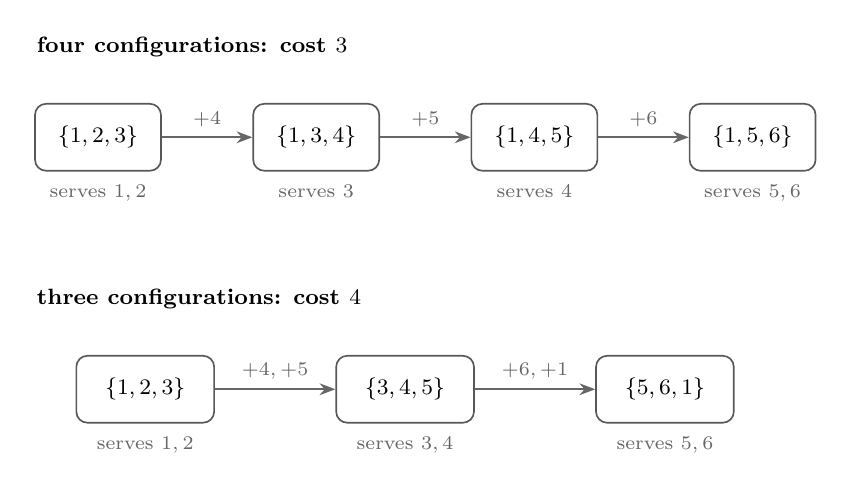
\begin{tikzpicture}[font=\footnotesize,>=Stealth,
   cfg/.style={draw=cPurple!70,semithick,fill=white,rounded corners,minimum width=1.6cm,minimum height=0.85cm},
   bad/.style={draw=cRed!70,semithick,fill=white,rounded corners,minimum width=1.75cm,minimum height=0.85cm},
   node distance=1.15cm]
 \begin{scope}
  \node[font=\footnotesize\bfseries,anchor=west] at (-0.9,1.15)
     {four configurations: cost $3$};
  \node[cfg] (c1) {$\{1,2,3\}$};
  \node[cfg,right=of c1] (c2) {$\{1,3,4\}$};
  \node[cfg,right=of c2] (c3) {$\{1,4,5\}$};
  \node[cfg,right=of c3] (c4) {$\{1,5,6\}$};
  \draw[->,semithick,black!60] (c1)--(c2) node[midway,above,font=\scriptsize]{$+4$};
  \draw[->,semithick,black!60] (c2)--(c3) node[midway,above,font=\scriptsize]{$+5$};
  \draw[->,semithick,black!60] (c3)--(c4) node[midway,above,font=\scriptsize]{$+6$};
  \node[below=0.5mm of c1,font=\scriptsize,text=black!60] {serves $1,2$};
  \node[below=0.5mm of c2,font=\scriptsize,text=black!60] {serves $3$};
  \node[below=0.5mm of c3,font=\scriptsize,text=black!60] {serves $4$};
  \node[below=0.5mm of c4,font=\scriptsize,text=black!60] {serves $5,6$};
 \end{scope}
 \begin{scope}[yshift=-3.2cm]
  \node[font=\footnotesize\bfseries,anchor=west] at (-0.9,1.15)
     {three configurations: cost $4$};
  \node[bad] (a) at (0.6,0) {$\{1,2,3\}$};
  \node[bad] (b) at (3.9,0) {$\{3,4,5\}$};
  \node[bad] (c) at (7.2,0) {$\{5,6,1\}$};
  \draw[->,semithick,black!60] (a)--(b) node[midway,above,font=\scriptsize]{$+4,+5$};
  \draw[->,semithick,black!60] (b)--(c) node[midway,above,font=\scriptsize]{$+6,+1$};
  \node[below=0.5mm of a,font=\scriptsize,text=black!60] {serves $1,2$};
  \node[below=0.5mm of b,font=\scriptsize,text=black!60] {serves $3,4$};
  \node[below=0.5mm of c,font=\scriptsize,text=black!60] {serves $5,6$};
 \end{scope}
\end{tikzpicture}
\caption{The $6$-ring in configuration space, in the walk model. Above: the optimal
schedule visits four configurations, each one tool from the next, for a cost of
three. Below: the heuristic may use only the $\Kst=3$ minimum-cardinality groups, and
every pair of the resulting configurations differs in two tools, so the best it can
do in this model is four. The extra unit is one re-insertion of tool~1, which the
middle configuration cannot hold. Figure~\ref{fig:frames} shows what happens when
the KTNS step is applied instead.}
\label{fig:gtsp}
\end{figure}

\subsection{Zero-gap classes and worst-case guarantees}\label{ssec:ratio}

This subsection proves bounds that hold for \emph{every} instance and every capacity.
Two quantities recur. The first is the tool excess $q=\lvert\U\rvert-b$ of
Section~\ref{ssec:lb}. The second is the number of \emph{re-insertions} a schedule
makes: insertions of tools that were in the magazine earlier and were removed. Write
$R_{\mathrm{opt}}$ for the re-insertions made by an optimal schedule. Throughout,
$\Kst\ge2$, since at $\Kst=1$ the heuristic is trivially exact, and all costs are
free-initial.

\begin{lemma}[Cost identity]\label{lem:costid}
Restrict every magazine state to a subset of $\U$, which is possible whenever
$\Kst\ge2$ and never increases cost. The free-initial cost of any full-magazine
schedule then equals $q+R$, where $R\ge0$ counts re-insertions.
\end{lemma}

\begin{proof}
Each of the $q$ tools of $\U$ outside the first fill is required by some job, so it
is inserted at least once. Split all insertions into first-time insertions, of which
there are exactly $q$, and the rest, which are by definition the $R$ re-insertions.
\end{proof}

Hence $\Zst=q+R_{\mathrm{opt}}$, and writing $R_{\mathrm{walk}}$ for the walk model's
re-insertions, $\Hwalk-\Zst=R_{\mathrm{walk}}-R_{\mathrm{opt}}$. The walk gap is
exactly the excess re-insertions forced by the cardinality restriction. On the
$6$-ring the single extra insertion is one such re-insertion: tool~1, needed by the
first and last groups but not the middle one, is removed at a group boundary and
reloaded (Figure~\ref{fig:frames}).

\begin{lemma}[Transition cap]\label{lem:transcap}
In any ordering of configurations contained in $\U$, every transition inserts at most
$\min(b,q)$ tools. Hence $\Hwalk\le(\Kst-1)\min(b,q)$.
\end{lemma}

\begin{proof}
A transition into $C_{k+1}$ inserts $\lvert C_{k+1}\setminus C_k\rvert$ tools. This
is at most $\lvert C_{k+1}\rvert=b$, and also at most
$\lvert\U\setminus C_k\rvert=q$, since $C_{k+1}\subseteq\U$ and
$\lvert C_k\rvert=b$. A covering configuration inside $\U$ exists for every group, so
some minimum-cardinality grouping uses only such configurations, and $\Hwalk$ is at
most its cost.
\end{proof}

These two lemmas give the section's central guarantee. Lemma~\ref{lem:transcap} caps
the heuristic's absolute cost, Corollary~\ref{cor:lb} floors the optimum, and
dividing one by the other bounds how far from optimal the method can stray.

\begin{theorem}[Worst-case guarantee]\label{thm:uncond}
For every instance with $\Kst\ge2$,
\[
  \frac{H}{\Zst}\ \le\ \frac{\Hwalk}{\Zst}
  \ \le\ \frac{(\Kst-1)\min(b,q)}{\max(\Kst-1,\ q)}
  \ \le\ \min\bigl(b,\ \Kst-1,\ q\bigr).
\]
More strongly, the same right-hand bound holds for the KTNS value $\widehat H$ of
\emph{every} job order obtained by concatenating the groups of any
minimum-cardinality grouping, in any group order and any within-group order.
\end{theorem}

\begin{proof}
For any such concatenated order, choose a covering configuration inside $\U$ for
each group and hold it while that group runs. Every transition costs at most
$\min(b,q)$ by Lemma~\ref{lem:transcap}, so KTNS optimality for the fixed order gives
$\widehat H\le(\Kst-1)\min(b,q)$. Proposition~\ref{prop:frames} gives
$H\le\Hwalk$, while Lemma~\ref{lem:transcap} gives the same absolute bound for
$\Hwalk$. Divide by $\Zst\ge\max(\Kst-1,q)\ge1$ (Corollary~\ref{cor:lb}). Finally,
$(\Kst-1)q/\max(\Kst-1,q)=\min(\Kst-1,q)$ together with $\min(b,q)\le q$
gives the $\min(\Kst-1,q)$ term, while $(\Kst-1)/\max(\Kst-1,q)\le1$ together with
$\min(b,q)\le b$ gives the $b$ term.
\end{proof}

This refines the $b$-approximation of \citet{CramaKlundert1999}. Their Theorem~8
shows that any solution of the job grouping problem yields a tool-switching solution of
cost at most $b$ times the grouping value, by the same construction studied here:
sequence the batches and pay at most $b$ switches between consecutive ones. In the
present notation that is $\Hwalk\le b(\Kst-1)$ against $\Zst\ge\Kst-1$. It was the bound the internship began
with. It tightens automatically on instances with few groups, with a small tool
excess, or with a small magazine.

\begin{corollary}[Zero-gap classes, every $b$]\label{cor:zerogap}
\emph{(i)} If $\Kst=2$ the gap is zero, and indeed $H=\Hwalk=\Zst=q$.
\emph{(ii)} If $\lvert\U\rvert\le b+1$ the gap is zero.
\emph{(iii)} If $\Kst=3$ then $H/\Zst\le2$.
\end{corollary}

\begin{proof}
The case $\Kst=1$ is trivial. Otherwise all three are instances of
Theorem~\ref{thm:uncond}, whose ratio bound is
$\Kst-1=1$, $q\le1$ and $\Kst-1=2$ respectively. For the equality in (i), pad the
first group's configuration to size $b$ using tools from the second group's
requirement, and pad the second from the first. The single transition then inserts
exactly the $q$ tools of $\U$ missing from the first configuration, so
$\Hwalk\le q\le\Zst\le H\le\Hwalk$ by the coverage bound.
\end{proof}

A positive gap therefore requires $\Kst\ge3$.

\begin{corollary}[Small optima are gap-free]\label{cor:smallZ}
If $\Zst\le2$ then the gap is zero, for every $b$ and every $\Kst$.
\end{corollary}

\begin{proof}
$\Zst\ge q$, so $q\le2$. If $q\le1$ the gap vanishes by
Corollary~\ref{cor:zerogap}(ii). If $q=2$ then $\Zst=q$, and the walk argument of
Appendix~\ref{app:proofs} yields a walk of at most $q+1=3$ configurations, each
serving a job, exhibiting a feasible grouping of that cardinality; for $\Kst\le2$ the
gap vanishes by Corollary~\ref{cor:zerogap}(i), and for $\Kst=3$ the walk grouping is
itself of minimum cardinality and has cost $\Zst$, forcing $\Hwalk=\Zst$.
\end{proof}

\begin{observation}[A small optimum does not force a unit walk gap]\label{obs:z3}
The conclusion of Corollary~\ref{cor:smallZ} cannot be extended from $2$ to $3$.
At $b=6$, the instance
\[
\begin{aligned}
T=\bigl(&\rset{0,1,4},\ \rset{0,2,3,5,6,7},\
\rset{0,3,6,8},\\
&\rset{4,5,7,8},\ \rset{6,7,8},\
\rset{1,5,6,7,8}\bigr)
\end{aligned}
\]
has $\Kst=3$, $q=\Zst=3$ and $\Hwalk=5$. Thus a walk gap of two is already possible
at optimum three. These values are exact-enumeration checks in
Appendix~\ref{app:verify}.
\end{observation}

\subsection{The extremal behaviour at three groups}\label{ssec:law}

Corollary~\ref{cor:zerogap} places every positive-gap instance at $\Kst\ge3$. This
subsection works out the case $\Kst=3$, which is where the extremes occur. All
results here are about the walk value; Section~\ref{ssec:ktnsgap} then asks what the
KTNS step does to them.

\begin{proposition}[Exact walk cost at $\Kst=3$]\label{prop:hk3}
If $\Kst=3$ then, with configurations restricted to subsets of $\U$,
\[
  \Hwalk\;=\;q\;+\;\min\ \min\bigl(x_{ab},\,x_{bc},\,x_{ca}\bigr),
  \qquad x_{uv}=\bigl\lvert(C_u\cap C_v)\setminus C_w\bigr\rvert,
\]
where the outer minimum runs over feasible $3$-groupings and choices of their
configurations, and $w$ denotes the third index in each case.
\end{proposition}

\begin{proof}
The three configurations of a feasible $3$-grouping are distinct, since two equal
ones would merge their groups and contradict $\Kst=3$, and together they cover $\U$.
For a path $(C_a,C_b,C_c)$, splitting the cost into first-time insertions and
re-insertions (Lemma~\ref{lem:costid}) gives cost
$q+\lvert(C_a\cap C_c)\setminus C_b\rvert$: the re-inserted tools are exactly those
of $C_c$ present in $C_a$ but absent from $C_b$. Minimising over the three possible
middle configurations selects the smallest of the three overlap terms, and $\Hwalk$
then minimises over groupings and configuration choices.
\end{proof}

This turns grouping selection at $\Kst=3$ into an explicit criterion: choose the
grouping whose configurations have the smallest pairwise overlap outside the third.
Section~\ref{ssec:grouping-sel} returns to it.

\begin{lemma}[Overlap counting]\label{lem:overlap}
Any three configurations $C_a,C_b,C_c\subseteq\U$ of size $b$ with
$C_a\cup C_b\cup C_c=\U$ satisfy
$\min(x_{ab},x_{bc},x_{ca})\le\lfloor(2b-q)/3\rfloor$.
\end{lemma}

\begin{proof}
Count tools by how many of the three configurations contain them. Let $a$ be the
number in exactly one, $\sum x:=x_{ab}+x_{bc}+x_{ca}$ the number in exactly two, and
$c_3$ the number in all three. Counting tools gives $a+\sum x+c_3=b+q$, and counting
memberships gives $a+2\sum x+3c_3=3b$. Subtracting, $\sum x=2b-q-2c_3\le2b-q$. The
minimum of three numbers is at most their mean, and it is an integer.
\end{proof}

\begin{proposition}[The walk gap at $\Kst=3$]\label{prop:k3}
Let $\Kst=3$ and $R_{\mathrm{opt}}=\Zst-q$. Then
\[
  \Hwalk-\Zst\ \le\ \max\Bigl(0,\ \min\bigl(q,\ \lfloor(2b-q)/3\rfloor\bigr)
  -R_{\mathrm{opt}}\Bigr).
\]
Consequently $\Hwalk-\Zst\le1$ holds
\emph{(i)} for every instance with $b\le4$;
\emph{(ii)} whenever $2b\le q+3R_{\mathrm{opt}}+5$;
\emph{(iii)} whenever $R_{\mathrm{opt}}\ge q-1$; and
\emph{(iv)} at $\Zst=q=3$ when some optimal four-configuration walk, after assigning
each job to a serving configuration, has two induced groups whose combined
requirement fits one magazine.
The bound can therefore fail only in the corner
$2b\ge q+3R_{\mathrm{opt}}+6$ with $R_{\mathrm{opt}}\le q-2$, which forces $b\ge5$.
\end{proposition}

\begin{proof}
The configurations of any feasible $3$-grouping cover $\U$, so
Proposition~\ref{prop:hk3} with Lemma~\ref{lem:overlap} gives
$\Hwalk\le q+\lfloor(2b-q)/3\rfloor$, while Lemma~\ref{lem:transcap} gives
$\Hwalk\le2\min(b,q)\le 2q$. Subtracting $\Zst=q+R_{\mathrm{opt}}$ yields the bound.
For (i) at $b=3$, $\lfloor(6-q)/3\rfloor\le1$ for every $q\ge1$. At $b=4$ the bound
is at most $1$ for $q\ge3$; for $q=2$, either $R_{\mathrm{opt}}\ge1$ and the bound is
at most $1$, or $\Zst=q\le2$ and the gap vanishes by Corollary~\ref{cor:smallZ}; and
$q\le1$ is Corollary~\ref{cor:zerogap}(ii). Parts (ii) and (iii) are read off the
bound, and part (iv) is proved in Appendix~\ref{app:proofs}.
\end{proof}

\begin{proposition}[A bound for every $\Kst$]\label{prop:genk}
For every instance with $\Kst\ge2$,
\[
  \Hwalk-\Zst\ \le\ \max\Bigl(0,\
  \Bigl\lfloor\frac{q\bigl(b(\Kst-1)-q\bigr)}{b+q}\Bigr\rfloor-R_{\mathrm{opt}}\Bigr).
\]
\end{proposition}

\begin{proof}
Fix a minimum-cardinality grouping. Its configurations $C_1,\dots,C_{\Kst}\subseteq\U$
are pairwise distinct and cover $\U$. In an ordering $\sigma$ the path cost is
$q+\sum_t(\mathrm{runs}_\sigma(t)-1)$, where $\mathrm{runs}_\sigma(t)$ counts the
maximal blocks of consecutive configurations containing $t$, since every block after
the first begins with a re-insertion (Lemma~\ref{lem:costid}). Let $d_t$ be the number
of configurations containing $t$, so that $\sum_t d_t=\Kst b$ over $b+q$ tools. Under
a uniformly random ordering,
$\mathbb{E}[\mathrm{runs}(t)-1]=(d_t-1)(\Kst-d_t)/\Kst$, which is concave in $d_t$, so
by Jensen's inequality the expected total excess is at most
$q\bigl(b(\Kst-1)-q\bigr)/(b+q)$. Some ordering achieves at most the mean, the total is
an integer, and subtracting $\Zst=q+R_{\mathrm{opt}}$ gives the claim.
\end{proof}

At $\Kst=3$ this and Proposition~\ref{prop:k3} are incomparable and both are attained
at the $6$-ring. Proposition~\ref{prop:genk} grows linearly in $\Kst$ and is
unconditional.

The next result shows that the natural guess $\mathrm{gap}\le\Kst-2$, which held on
all the evidence collected before this internship, is false for the walk value. All
the earlier evidence lay at $b\le4$, which is exactly the region
Proposition~\ref{prop:k3} proves.

\begin{observation}[The $\Kst-2$ bound fails for the walk value]\label{obs:refute}
There are instances with $\Kst=3$ and $\Hwalk-\Zst=2$. One, with $b=5$ and
$\U=\rset{1,\dots,9}$, is
\[
  W:\quad T=\bigl(\rset{1,2,3,5,8},\ \rset{1,5,6},\ \rset{2,6},\ \rset{3,7,9},\
  \rset{4,5,6,9}\bigr),
\]
with $q=4$, $\Zst=4$ and $\Hwalk=6$, both values obtained by exhaustive computation.
The instance lies exactly on the boundary of the regimes of
Proposition~\ref{prop:k3}, at $2b=q+3R_{\mathrm{opt}}+6$, and attains that
proposition's bound with equality.
\end{observation}

\begin{observation}\label{obs:refute-ktns}
On the same instance $W$, the KTNS step gives $H=5$, so the heuristic gap is one and
the guess $\mathrm{gap}\le\Kst-2$ is not contradicted by it.
\end{observation}

\begin{conjecture}[The $4/3$ walk ratio at $b=3$]\label{conj:43}
For every instance with $b=3$, $\Hwalk/\Zst\le4/3$ (and therefore
$H/\Zst\le4/3$).
\end{conjecture}

The evidence is a complete enumeration of two families. The first is every instance
in which each job requires exactly two tools, with $b=3$, at most six tools and at
most six jobs: $10{,}691$ instances, of which the maximum ratio is exactly $4/3$,
attained at the $6$-ring in the walk model. The second is every instance with $b=3$
whose jobs require two or three tools, with at most five tools and at most five jobs:
a further $6{,}065$ instances, none exceeding $4/3$.

\begin{proposition}[The $4/3$ bound holds whenever $\Kst\le3$]\label{prop:43route}
Every instance with $b=3$ and $\Kst\le3$ satisfies $\Hwalk/\Zst\le4/3$, and hence
$H/\Zst\le4/3$. Conjecture~\ref{conj:43} is therefore open only for $\Kst\ge4$.
\end{proposition}

\begin{proof}
For $\Kst\le2$ the gap is zero (Corollary~\ref{cor:zerogap}). For $\Kst=3$,
Proposition~\ref{prop:k3}(i) gives a walk gap of at most one, and a positive gap
forces $\Zst\ge3$ (Corollary~\ref{cor:smallZ}), so
$\Hwalk/\Zst=1+(\Hwalk-\Zst)/\Zst\le1+1/3$. Proposition~\ref{prop:frames} carries the
bound to $H$.
\end{proof}

The reduction to $\Kst\ge4$ is not vacuous. Positive-walk-gap instances with $b=3$
and $\Kst=4$ exist; one is
$T=(\rset{1,3,6},\rset{1,4,7},\rset{2,3},\rset{2,5},\rset{2,7})$, with $\Zst=4$ and
$\Hwalk=5$. No ratio above $4/3$ has been found in that regime.

\subsection{What the KTNS step does to the walk gap}\label{ssec:ktnsgap}

Everything in Section~\ref{ssec:law} bounds $\Hwalk$. By
Proposition~\ref{prop:frames} those bounds also hold for $H$. The question this
subsection asks is how much slack that inequality hides. The answer is: a great deal,
and on exactly the instances the literature uses as examples.

\begin{observation}[The ring family has no heuristic gap]\label{obs:rings}
For the $k$-ring at $b=3$ with $k=3,\dots,9$, the heuristic is optimal:
$H=\Zst$ in every case. The walk value is one above the optimum for
$k=6,\dots,9$. Table~\ref{tab:rings} gives the values.
\end{observation}

\begin{table}[h]\centering
\begin{tabular}{ccccccc}
\toprule
$k$ & $\Kst$ & $\Zst$ & $\Hwalk$ & walk gap & $H$ & heuristic gap\\
\midrule
3 & 1 & 0 & 0 & 0 & 0 & 0\\
4 & 2 & 1 & 1 & 0 & 1 & 0\\
5 & 3 & 2 & 2 & 0 & 2 & 0\\
6 & 3 & 3 & 4 & 1 & 3 & 0\\
7 & 4 & 4 & 5 & 1 & 4 & 0\\
8 & 4 & 5 & 6 & 1 & 5 & 0\\
9 & 5 & 6 & 7 & 1 & 6 & 0\\
\bottomrule
\end{tabular}
\caption{The $k$-ring at $b=3$, free-initial costs, computed exhaustively. The walk
value separates from the optimum at $k=6$ and stays one above it. The value the
heuristic actually returns equals the optimum for every $k$ tested. The mechanism is
the one drawn in Figure~\ref{fig:frames}.}\label{tab:rings}
\end{table}

This is why the distinction of Section~\ref{ssec:frames} cannot be dropped. The
$6$-ring is the standard example of a positive gap for this heuristic, and for the
heuristic as defined it has no gap at all. The same holds for the $\Kst=4$ instance
at the end of Section~\ref{ssec:law}, whose walk gap is one and whose heuristic gap
  is zero, and for the witness $W$ of Observation~\ref{obs:refute}, whose walk gap is
two and whose heuristic gap is one.

Positive heuristic gaps do exist. They are simply rarer and smaller than the walk
model suggests.

\begin{proposition}[The smallest sub-optimal instance]\label{prop:seed}
Four jobs are necessary and sufficient for a positive heuristic gap. A smallest
witness, with $b=4$ and $\U=\rset{1,\dots,7}$, is
\[
  A=\rset{1,2},\quad B=\rset{3,4},\quad
  C=\rset{1,3,5,6},\quad D=\rset{2,5,6,7}.
\]
It has $\Kst=3$, $\Zst=3$ and $H=4$.
\end{proposition}

\begin{proof}
The only feasible pair is $\rset{A,B}$, so every minimum grouping is
$\rset{\rset{A,B},\rset C,\rset D}$ and $\Kst=3$. The coverage bound is $q=3$.
The order $B,C,A,D$ admits the magazines
\[
 \rset{1,3,4,5}\to\rset{1,3,5,6}\to
 \rset{1,2,5,6}\to\rset{2,5,6,7},
\]
so it attains that bound and $\Zst=3$. A grouped order must place $A$ and $B$
consecutively. Up to reversal, its six possibilities have the following exact
KTNS values:
\[
\begin{array}{c|rrrrrr}
\text{order}&ABCD&ABDC&BACD&BADC&CABD&CBAD\\\hline
\KTNS&4&5&4&5&4&4 .
\end{array}
\]
Thus $H=4$. Finally, an instance with at most three jobs either has
$\Kst\le2$, when Corollary~\ref{cor:zerogap} applies, or has three singleton
groups, in which case every job permutation is available to the heuristic and
$H=\Zst$. Hence four jobs are necessary.
\end{proof}

\begin{observation}[Positive heuristic gaps are rare and small]\label{obs:census}
Draw instances with a uniformly random requirement of admissible size for each job. In
$1{,}260$ instances with three to five jobs, four to eight tools and capacity between
two and five, drawn as three independent samples of $420$ with pseudorandom seeds
$0,1,2$, \emph{none} has $H>\Zst$.
This fixed census is reproduced by the independent verifier. It is a frequency
statement about that sample only: Proposition~\ref{prop:seed} gives a positive gap,
and Theorem~\ref{thm:connected-gap} below proves that connected instances can have
arbitrarily large gaps.

Capacity three already admits a positive gap. The following retained five-job,
seven-tool witness has
\[
  T_1=\rset{4,6},\quad T_2=\rset{0,1,3},\quad T_3=\rset{1,6},\quad
  T_4=\rset{0,5,6},\quad T_5=\rset{4,5,7},
\]
with $\Kst=4$, $\Zst=4$ and $H=5$.
\end{observation}

\begin{remark}[A correction]\label{rem:census-b3}
An earlier draft of this report stated that every instance carrying a positive heuristic
gap has $b\ge4$, on the strength of the $1{,}260$-instance census alone. The witness
above refutes that: it has $b=3$. What survives is only the reproducible statement that
the fixed three-to-five-job census found no gap, together with the checked witness that
shows absence from that sample is not a structural threshold. No claim about the
frequency at $b=3$, or about general absence at $b=2$, is made.
\end{remark}

The capacity condition matters. A positive heuristic gap
needs the magazine to be large relative to the jobs. That is the regime
in which \citet{Burger2015} report the decomposition degrading: as the difference
between the magazine size and the largest job size grows, the quality of the
heuristic's solutions decreases. Their finding is empirical and industrial, while
Proposition~\ref{prop:seed} is an exact combinatorial witness, and the regimes agree.

The walk gap and the actual heuristic gap are both unbounded, but require different
families.

\begin{proposition}[Unbounded walk gap]\label{prop:unbounded}
Let $R_g$ consist of $g$ tool-disjoint copies of the $6$-ring, so that $b=3$ and
$\lvert\U\rvert=6g$. Then $\Zst=6g-3$ and $\Hwalk=7g-3$, so the walk gap $g$ grows
without bound, while the walk ratio $(7g-3)/(6g-3)$ decreases from $4/3$ towards
$7/6$.
\end{proposition}

The proof is in Appendix~\ref{app:proofs}. It pairs the coverage bound with an
explicit schedule attaining it, and counts the heuristic's cost as $g$ within-copy
contributions of four and $g-1$ inter-copy transitions of three.

By Observation~\ref{obs:rings} this construction says nothing about $H$: the ring has
no heuristic gap, so copies of it have none either. Replacing the seed repairs the
construction.

\begin{observation}[A candidate disconnected family]\label{obs:copies}
Let $S$ be the four-job instance of Proposition~\ref{prop:seed}, which has $b=4$,
$\lvert\U\rvert=7$ and heuristic gap one, and let $S_g$ consist of $g$ tool-disjoint
copies of it. Exhaustive computation gives
\[
  \begin{array}{c|ccccc}
   g & \lvert\U\rvert & \Kst & \Zst & H & H-\Zst\\\hline
   1 & 7  & 3 & 3  & 4  & 1\\
   2 & 14 & 6 & 10 & 12 & 2
  \end{array}
\]
so $\Zst=7g-4=\lvert\U\rvert-b$ and the heuristic gap equals $g$ on both.
\end{observation}

\begin{conjecture}\label{conj:disconnected}
For every $g\ge1$ the instance $S_g$ of Observation~\ref{obs:copies} has
$\Zst=7g-4$ and $H-\Zst=g$. In particular the heuristic gap is unbounded.
\end{conjecture}

\begin{support}
The optimum is immediate: the coverage bound gives $\Zst\ge7g-4$, and processing the
copies one after another, each by its own optimal schedule, attains it, because
consecutive copies are tool-disjoint and so the magazine must be rebuilt in full
between them. For $H$ the difficulty is that a group may in principle contain jobs
from two different copies, since two jobs requiring two tools each can together
require exactly $b=4$. Verifying that no such grouping helps is what the computation
above does, and what a proof would have to establish in general.
\end{support}

The cross-copy grouping obstruction can be removed by connecting the copies while
making their minimum grouping unique.

\begin{theorem}[Connected unbounded heuristic gap]\label{thm:connected-gap}
For every $g\ge1$ there is a connected instance with capacity $b=6$ such that
\[
  \lvert\U\rvert=8g+1,\qquad \Kst=3g,\qquad
  \Zst=8g-5,\qquad H=9g-5.
\]
Consequently $H-\Zst=g$: the actual KTNS-postprocessed heuristic has an unbounded
gap even on connected instances.
\end{theorem}

\begin{proof}
Take $g$ private copies of the seven tools and four jobs $A,B,C,D$ of
Proposition~\ref{prop:seed}. Add one universal tool $u$ to every job, and for each
copy $i$ add a private marker $v_i$ to all four jobs of that copy. Every large job
$C_i,D_i$ now fills all six slots and can share no group. The two small jobs
$A_i,B_i$ of one copy use six tools together and form a feasible pair, whereas two
small jobs from different copies use seven tools because their original and marker
tools are disjoint. Hence the unique minimum grouping has
$\rset{A_i,B_i},\rset{C_i},\rset{D_i}$ for every $i$, and $\Kst=3g$.

There are seven original tools and one marker per copy, plus $u$, so
$q=\lvert\U\rvert-b=8g-5$. Process the copies consecutively, using the
zero-reinsertion order $B_i,C_i,A_i,D_i$ displayed in the proof of
Proposition~\ref{prop:seed}. Keep $u$ throughout. Within a copy, $v_i$ occupies one
slot and the original tools reproduce that four-slot loading; on entering the next
copy all newly loaded private tools are first occurrences. Thus no tool is
reinserted and the coverage bound is attained: $\Zst=q$.

Now take any order admitted by a minimum grouping. Within every copy, $A_i$ and
$B_i$ are consecutive. At a job of copy $i$, the required tools $u,v_i$ leave at
most four slots for that copy's seven original tools. If none of those private
original tools were reinserted, restricting the loading to the four jobs and seven
tools of copy $i$ would give a capacity-four, zero-reinsertion loading of a seed
order with $A,B$ consecutive. The KTNS table in Proposition~\ref{prop:seed} proves
that no such loading exists. More explicitly, let $x_i$ count original tools of
copy $i$ in the free initial magazine and let $y$ count initially loaded tools among
$\rset{u,v_1,\ldots,v_g}$. Copy $i$ therefore needs at least $8-x_i$ later
insertions (its $7-x_i$ first occurrences plus one re-insertion), while the common
and marker tools need at least $g+1-y$. Since $\sum_i x_i+y\le6$, every admitted
order costs at least
\[
  \sum_i(8-x_i)+(g+1-y)\ \ge\ 9g-5=q+g.
\]

Finally, process the copies consecutively in the grouped order $A_i,B_i,C_i,D_i$.
The same table gives exactly one private reinsertion per copy and no cross-copy
reinsertion, so the cost is $q+g=9g-5$. This proves the formula for $H$. Since every
job contains $u$, both the job-intersection graph and the job--tool incidence graph
are connected.
\end{proof}

Finally, the phenomenon behind all of this is best stated as a question, since
it is the natural one to ask next and it has no answer here.

\begin{problem}\label{prob:ktns-closes}
Characterise the instances on which the KTNS step closes the walk gap, that is, on
which $H<\Hwalk$. Equivalently: when does re-optimising the loading over the whole
flattened order recover an optimum that no single magazine per group can reach?
\end{problem}

The evidence assembled here is that this happens very often, and that the walk model
therefore substantially overstates the weakness of the standard method.

\subsection{What the gap does not depend on}\label{ssec:clutter}

The results above are quantitative. This subsection asks from which combinatorial
structure of an instance the gap could, even in principle, be read. The natural
object is the family of feasible groups.

\begin{definition}[Group complex and circuit clutter]\label{def:complex}
Let $\mathcal{F}=\rset{S\subseteq J:\lvert\bigcup_{j\in S}T_j\rvert\le b}$. Since
$\lvert T_j\rvert\le b$ and membership is preserved under taking subsets,
$\mathcal{F}$ is an independence system on $J$. Its inclusion-minimal non-members,
the \emph{circuits}, form a clutter $\mathcal{C}$.
\end{definition}

Three plain ideas sit in that definition. That $\mathcal{F}$ is an independence system
means only that feasibility is preserved downwards: remove a job from a group that
fits, and it still fits. The circuits are the minimal ways to fail: a set of jobs
whose tools overflow the magazine although every proper subset fits. A clutter is a
family no member of which contains another, which the circuits form automatically.

\begin{proposition}[$\Kst$ is a hypergraph chromatic number]\label{prop:chromK}
A set of jobs is a feasible group if and only if it contains no circuit. Hence $\Kst$
is the chromatic number of the hypergraph $(J,\mathcal{C})$. The \emph{conflict
graph}, whose edges join pairs of jobs that cannot share a configuration, consists
exactly of the two-element circuits, so its chromatic number is at most $\Kst$ and
may be strictly smaller. For $T_1=\rset{1,2}$, $T_2=\rset{1,3}$, $T_3=\rset{1,4}$
with $b=3$ there is no conflicting pair at all, yet the three jobs together require
four tools, so they form a circuit and $\Kst=2$.
\end{proposition}

\begin{proof}
An infeasible set contains a minimal infeasible subset and feasibility is preserved
downwards, which gives the first claim. Colour classes of a proper colouring of
$(J,\mathcal{C})$ are then exactly feasible groups. Two-element circuits are precisely
the conflicting pairs, and every proper colouring of the hypergraph properly colours
the graph. The stated instance computes as claimed.
\end{proof}

Figure~\ref{fig:hypergraph} draws the example. The point it makes is that pairwise
conflicts undercount: three jobs can be pairwise compatible and jointly infeasible,
so the true obstruction is the hypergraph of all minimal clashes.

\begin{figure}[ht]\centering
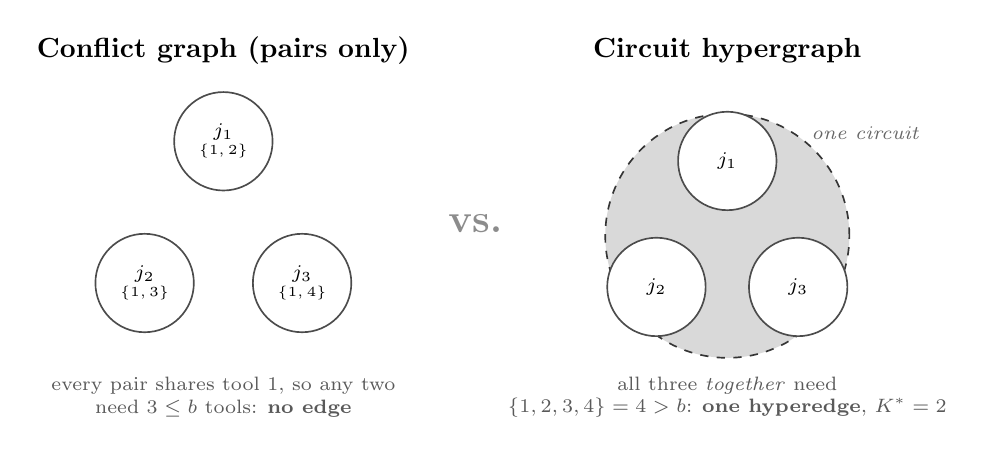
\begin{tikzpicture}[font=\small,>=Stealth,
   jb/.style={draw=cPurple!75,fill=white,circle,semithick,minimum size=1.25cm,
              inner sep=0pt,align=center,font=\scriptsize\bfseries}]
  \node[font=\bfseries] at (1.4,2.55) {Conflict graph (pairs only)};
  \node[jb] (a1) at (1.4,1.4)  {$j_1$\\[-1.5pt]{\tiny$\{1,2\}$}};
  \node[jb] (b1) at (0.4,-0.4) {$j_2$\\[-1.5pt]{\tiny$\{1,3\}$}};
  \node[jb] (c1) at (2.4,-0.4) {$j_3$\\[-1.5pt]{\tiny$\{1,4\}$}};
  \node[align=center,font=\scriptsize,text=black!65] at (1.4,-1.85)
     {every pair shares tool $1$, so any two\\ need $3\le b$ tools: \textbf{no edge}};
  \node[font=\Large\bfseries,text=black!45] at (4.6,0.35) {vs.};
  \node[font=\bfseries] at (7.8,2.55) {Circuit hypergraph};
  \begin{scope}[on background layer]
    \fill[cOrange!16] (7.8,0.2) circle (1.55);
    \draw[cOrange!85,semithick,dashed] (7.8,0.2) circle (1.55);
  \end{scope}
  \node[jb] (a2) at (7.8,1.15)  {$j_1$};
  \node[jb] (b2) at (6.9,-0.45) {$j_2$};
  \node[jb] (c2) at (8.7,-0.45) {$j_3$};
  \node[text=black!60,font=\scriptsize\itshape] at (9.55,1.5) {one circuit};
  \node[align=center,font=\scriptsize,text=black!65] at (7.8,-1.85)
     {all three \emph{together} need\\ $\{1,2,3,4\}=4>b$: \textbf{one hyperedge}, $\Kst=2$};
\end{tikzpicture}
\caption{Why $\Kst$ is read off the hypergraph of all minimal clashes and never off
the graph of pairwise ones. On this instance no two jobs conflict, because any two of
them need only three tools, which fit. All three together need four and overflow the
magazine, so they form a circuit, and that single circuit already forces two groups.}
\label{fig:hypergraph}
\end{figure}

\begin{proposition}[No matroid structure]\label{prop:nonmatroid}
$\mathcal{F}$ is not a matroid in general. For $T_1=\rset{1}$, $T_2=\rset{2}$,
$T_3=\rset{3,4}$ with $b=2$, both $\rset{3}$ and $\rset{1,2}$ are independent, but
neither $\rset{1,3}$ nor $\rset{2,3}$ is, so the exchange axiom fails. Greedy and
matroid-union arguments are therefore unavailable without further hypotheses.
\end{proposition}

\begin{proof}
The relevant unions have sizes $2$, $2$, $3$ and $3$.
\end{proof}

\begin{observation}[The circuit clutter does not determine the gap]\label{obs:noclutter}
Two instances with $b=4$, $\lvert\U\rvert=7$, four jobs, isomorphic circuit clutters
and equal $\Kst=3$ and $\Zst=3$ can have different gaps:
\[
\begin{aligned}
  I_0:\ &T=\bigl(\rset{1,3,7},\ \rset{2,3,4},\ \rset{3,4,5,6},\ \rset{4,5,6}\bigr),\\
  I_1:\ &T=\bigl(\rset{1,2,4,7},\ \rset{2,5,6,7},\ \rset{3,5},\ \rset{4,6}\bigr).
\end{aligned}
\]
In both, every pair of jobs conflicts except the last two, and no larger set is a
minimal clash. Yet $I_0$ has gap zero and $I_1$ has gap one, in both the walk value
and the heuristic value.
\end{observation}

The pairwise union sizes are checked directly. The displayed objective values are
obtained by exact enumeration over sequences and minimum-cardinality groupings in
the independent verifier; this is why the statement is classified as an Observation.

No criterion that reads only the circuit clutter, and a fortiori none that reads only
the conflict graph, can therefore decide when the gap vanishes. Tool-level structure
is essential, and that is exactly the level at which Proposition~\ref{prop:hk3}
operates: its overlap sizes $x_{uv}$ are precisely the data the clutter forgets.

On the covering side, however, the clutter is the right object, and blocking duality
makes this precise.

\begin{proposition}[Circuit--group blocking identity]\label{prop:circblocker}
On ground set $J$, the blocker of the circuit clutter, meaning the clutter of its
minimal transversals, is the family of minimal complements of maximal feasible
groups.
\end{proposition}

\begin{proof}
A set meets every circuit if and only if its complement contains no circuit, if and
only if its complement is a feasible group. Minimal transversals therefore correspond
to maximal feasible complements.
\end{proof}

This has a concrete consequence for the next section. Grouping branch-and-price rests
on a set-covering relaxation, and it is fast only when that relaxation is
\emph{ideal}, meaning its fractional optimum is already integral. The next result
exhibits the smallest family where it is not.

\begin{proposition}[Odd rings are not ideal]\label{prop:oddring}
Consider the JGP set-covering formulation with one column for each maximal feasible
group. On the $k$-ring with $b=3$ and $k\ge4$, its fractional optimum equals $k/2$ while
$\Kst=\lceil k/2\rceil$. The covering relaxation is therefore tight for every even
$k$ and has integrality gap $\tfrac12$ for every odd $k$.
\end{proposition}

\begin{proof}
For $k\ge4$ the maximal feasible groups are exactly the pairs of adjacent jobs.
Weight $\tfrac12$ on each covers every job exactly once, so the fractional cover is at
most $k/2$. The dual packing $y_j=\tfrac12$ is feasible, since no group holds more than
two jobs, so by linear-programming duality the fractional cover equals $k/2$. The
integer optimum is $\lceil k/2\rceil$.
\end{proof}

The hypothesis $k\ge4$ is needed: at $k=3$ all three jobs require only the three tools
$\rset{1,2,3}$, so the whole job set is one feasible group and $\Kst=1$.

This locates a first provable obstruction for the set-covering relaxation behind
grouping branch-and-price \citep{Crama1994Column,Otiai2026}: odd circular structure,
in exact parallel to odd holes in perfect-graph theory \citep{Chudnovsky2006}.

It is natural to ask whether it is the \emph{only} obstruction. At $b=3$ with every job
requiring exactly two tools the question is finite, because the family is then a family
of graphs: a tool is a vertex, a job is an edge, and a feasible group is a set of edges
spanning at most three vertices. The $k$-ring is the cycle $C_k$. Every such instance up
to isomorphism on at most six tools can therefore be enumerated and tested, and the
answer is negative.

\begin{proposition}[A non-ring obstruction]\label{prop:starobstruction}
At $b=3$ the three-job star
\[
  T_1=\rset{a,b},\qquad T_2=\rset{a,c},\qquad T_3=\rset{a,d}
\]
has fractional cover $\tfrac32$ and $\Kst=2$. It contains no odd cycle, so odd-ring
structure among the tools is not necessary for the covering relaxation to be
non-integral.
\end{proposition}

\begin{proof}
Any two of the three jobs together require three tools and form a feasible group; all
three require four and do not. The maximal feasible groups are therefore the three
pairs, and each job lies in exactly two of them, so weight $\tfrac12$ on each pair
covers every job and the fractional cover is at most $\tfrac32$. The dual packing
$y_j=\tfrac12$ is feasible because no group holds more than two jobs, so by
linear-programming duality the fractional cover equals $\tfrac32$. No single group holds
all three jobs, so $\Kst=2$. The tool graph is the star $K_{1,3}$, which is bipartite.
\end{proof}

\begin{observation}[How common the obstruction is]\label{obs:starobstruction}
Of the $155$ instances of this family with at most six tools, exactly $80$ have a
non-integral covering relaxation. Eleven of those are bipartite. The star of
Proposition~\ref{prop:starobstruction}, with three jobs, is the smallest non-integral
instance of the family; the smallest ring witness has five.
\end{observation}

What the star and the odd ring share is not circular structure among the \emph{tools} ---
the star has none --- but odd structure among the \emph{jobs}: in both cases three jobs
are pairwise compatible and not jointly compatible. That is the odd hole, seen in the compatibility hypergraph on jobs
rather than in the graph on tools, and it is where a characterisation should be sought.
Section~\ref{ssec:further} records what remains open.

\subsection{The setup-cost spectrum}\label{ssec:collapse}

In practice a machine stop costs time beyond the individual tool exchanges. This
subsection shows that the SSP and the JGP are the two ends of a single parameterised
problem, with the transition governed by the gap itself. The weighted objective is
established rather than new: \citet{Salonen2006} minimise a weighted sum of setup
occasions and feeder changes, and \citet{Burger2015} return to the trade-off.
\citet{Furrer2017} study a related fixed-order, lexicographic version. The contribution
below is the structural collapse threshold for variable-order,
fixed-configuration schedules.

Charge, in addition to the tool switches, a cost $\rho\ge0$ for every
\emph{configuration change}. The objective becomes
\[
  \text{switches}\;+\;\rho\cdot(\text{number of configuration changes}),
\]
where $\rho$ is the ratio of the fixed stop time to the time of one tool exchange. A
grouping into $p$ configurations makes $p-1$ changes, so the setup term alone is
minimised by the Job Grouping Problem. As $\rho$ grows it dominates and pulls the
optimum onto minimum-cardinality groupings.

For precision, a \emph{fixed-configuration group walk} chooses a feasible grouping
$\mathcal P=(G_1,\ldots,G_p)$ and full magazine configurations
$C_1,\ldots,C_p$, holds $C_\ell$ unchanged while processing the jobs of $G_\ell$,
and changes configuration only between groups. Its augmented cost is
\[
  \sum_{\ell=1}^{p-1}|C_{\ell+1}\setminus C_\ell|+\rho(p-1).
\]
This is the walk frame of Definition~\ref{def:frames}; it is not the KTNS
post-processing step of the standard heuristic.

\begin{theorem}[Setup-cost collapse for configuration schedules]\label{thm:collapse}
If $\rho>\Hwalk-\Zst$, then every optimum of the setup-augmented configuration-schedule
problem has exactly $\Kst$ maximal blocks of identical magazine configurations, and
its value is
\[
  \Hwalk+\rho(\Kst-1).
\]
Consequently a cheapest minimum-cardinality fixed-configuration group walk is exact.
\end{theorem}

\begin{proof}
Collapse consecutive equal configurations in any feasible schedule into $r$ maximal
blocks. The jobs processed in each block form a feasible group, so $r\ge\Kst$; and
the switching part is a feasible configuration walk, so by
Theorem~\ref{thm:grouping} it is at least $\Zst$. The augmented cost is therefore at
least $\Zst+\rho(r-1)$. A cheapest minimum-cardinality fixed-configuration group walk
has cost $\Hwalk+\rho(\Kst-1)$. If $r>\Kst$, the lower bound exceeds that candidate
whenever
\[
  \rho(r-\Kst)>\Hwalk-\Zst,
\]
which follows from $\rho>\Hwalk-\Zst$. Hence every optimum has $r=\Kst$. Among
schedules with exactly $\Kst$ configuration blocks, the least possible switching part
is precisely $\Hwalk$, proving the displayed value and exactness of the fixed-walk
construction.
\end{proof}

If $\rho_c$ denotes the infimum of values above which every optimum has exactly
$\Kst$ blocks, the theorem gives the sufficient bound
$\rho_c\le\Hwalk-\Zst$. No claim of equality is needed for the result.

The threshold must be read in the walk value. Substituting $H$ does not repair or
strengthen the statement: KTNS can reduce the number of switches by visiting extra
magazine states inside the selected groups, and $H$ records no corresponding number of
configuration changes. Thus Theorem~\ref{thm:collapse} does not say that the ordinary
KTNS-evaluated two-phase heuristic is exact for the augmented objective; such a
heuristic would need a selection rule that optimises both terms.

\begin{lemma}[The other end of the spectrum]\label{lem:lowrho}
If $n\ge2$ and $\rho<1/(n-1)$, every optimum of the setup-augmented objective is a
switch-optimal SSP schedule.
\end{lemma}

\begin{proof}
A schedule makes at most $n-1$ configuration changes. Let $S^{*}$ be switch-optimal.
Any schedule with at least $\Zst+1$ switches has augmented cost at least
$\Zst+1>\Zst+\rho(n-1)$, which is at least the augmented cost of $S^{*}$. No such
schedule is therefore optimal.
\end{proof}

Together these pin both ends. For $\rho<1/(n-1)$ the augmented problem is the SSP.
For $\rho>\Hwalk-\Zst$ every optimum uses the minimum number of configuration blocks,
and the fixed-configuration walk is exact, so the primary objective has collapsed onto
the JGP while switching cost breaks ties. Where a transition interval remains, its
upper endpoint is the walk gap $\Hwalk-\Zst$. This is a statement about the explicit
configuration-schedule model, not an exactness claim for KTNS post-processing.

\begin{remark}[On practical values of $\rho$]\label{rem:rho}
It is natural to ask where real manufacturing sits on this spectrum. Answering that
requires measured values of the stop time and the per-tool exchange time in a
comparable setting, and no source giving both could be found during this internship.
The spectrum result is therefore stated as it is proved, as a statement about the
parameter $\rho$, and no claim is made about where practice falls on it. Obtaining
such measurements would settle a question that Theorem~\ref{thm:collapse} otherwise
leaves open.
\end{remark}

\subsection{Which grouping to choose}\label{ssec:grouping-sel}

Theorem~\ref{thm:grouping} turns the heuristic's weakness into a concrete algorithmic
question. The optimum is attained by \emph{some} feasible grouping, and
minimum-cardinality ones may miss it (Example~\ref{ex:ring-why}). On which grouping,
then, should the sequencing phase be run?

Admitting a single extra group already recovers the ring optimum in the walk model. In
general the trade-off is between more configuration changes and cheaper individual
transitions. At $\Kst=3$, Proposition~\ref{prop:hk3} makes the criterion explicit:
choose the grouping whose configurations have the smallest pairwise overlap outside
the third. For general $\Kst$, characterising the groupings that attain
$\min_{\mathcal{P}}\gamma(\mathcal{P})$, or giving an efficient rule that improves on
the minimum-cardinality choice, is open.

Two things follow from Section~\ref{ssec:ktnsgap}. The
first is that the practical value of such a rule is smaller than the walk model
suggests, since the KTNS step already recovers the optimum on most instances where
the walk model loses it. The second is that the instances where a rule would help are
identifiable in advance by the same criterion that identifies positive gaps: a
magazine large relative to the jobs.

%==============================================================================
\section{Exact methods}\label{sec:exact}
%==============================================================================

Section~\ref{sec:gap} showed that the coverage bound $q=\lvert\U\rvert-b$ equals the
optimum on a large part of the instance space. Section~\ref{sec:sota} showed that the
strongest of the compact formulations reimplemented here has a linear relaxation equal to that
same quantity. This section asks whether an exact method can do better, and builds
two that are designed to.

\paragraph{Why these two methods.}
A compact integer formulation is the natural first recourse, and three from the
literature serve here as baselines. Their relaxations do not exceed the coverage
bound, so a branch-and-cut built on any of them is fast where that bound is tight and
adrift where it is not. Escaping this requires a method that does not rest on a
compact relaxation, and two classical routes qualify, for opposite reasons.

Benders decomposition is the textbook fit when the subproblem is polynomially
solvable \citep{Rahmaniani2017}. The loading problem is such a subproblem, so it
becomes an oracle returning exact cuts, and the master's bound is assembled from true
subproblem values rather than from a linear relaxation of the loading. The algorithm
never forms that relaxation at all --- which is a statement about the loading and not
about the master, whose own root bound Observation~\ref{obs:rootq} finds sitting on the
coverage row on $87.2\%$ of recorded runs. This places the solver in the lineage of logic-based
\citep{Hooker2003} and combinatorial \citep{Codato2006} Benders decomposition.

Branch-and-price attacks the same weakness from the other side. Reformulating over
configurations, its position--transition variant carries a relaxation that can provably
exceed the coverage bound (Proposition~\ref{prop:ptf}), which is the one construction in
this report that does. How often it does so on real instances is a separate question,
and Section~\ref{ssec:results-bnp} answers it.

\begin{table}[t]\centering
\footnotesize
\begin{tabular}{@{}llll@{}}
\toprule
Method & Source & Formulation & Linear relaxation \\
\midrule
F4          & \citet{Catanzaro2015} & compact, arc-based            & in general below $q$ \\
LSS         & \citet{Laporte2004}   & compact, tool-state           & in general below $q$ \\
SSPMF       & \citet{daSilva2024}   & multicommodity flow           & $=q$ when every tool is used \\
BBC         & this work             & branch-and-Benders-cut        & no relaxation of the loading \\
PCF, PCF$'$ & this work             & position--configuration B\&P  & $=q$ with the counting rows \\
PTF         & this work             & position--transition B\&P     & $\ge q$, and can exceed it \\
\bottomrule
\end{tabular}
\caption{The three compact baselines and the methods of this report, ordered by the
strength of their linear relaxation relative to the coverage bound $q$. Every method
is exact; they differ in whether, and by what means, they get past that bound. The
entries for F4 and LSS are hedged because the source states only that earlier models
fall below $q$ in the great majority of cases \citep{daSilva2024}, not in all.}
\label{tab:methods}
\end{table}

\subsection{Compact formulations and the limit they reach}\label{ssec:compact}

Three compact formulations from the literature serve as baselines: Formulation~4 of
\citet{Catanzaro2015}, the tool-state model of \citet{Laporte2004}, and the
multicommodity-flow model of \citet{daSilva2024}. Section~\ref{ssec:sota-compact}
describes all three and records the omission of the stronger Formulation~5 as a
limitation. All three were reimplemented for this study, and
Section~\ref{ssec:validation} describes how they were checked. The last is singled out
here by its relaxation.

\begin{proposition}[\citealp{daSilva2024}]\label{prop:sspmf-lp}
The linear relaxation of the multicommodity-flow formulation equals
$\lvert T\rvert-b$, the number of tools minus the magazine capacity. Under the
standing assumption that every tool is required by some job, so that $\U=T$, this is
the coverage bound $q$ of Proposition~\ref{prop:lb2}.
\end{proposition}

The hypothesis matters and is stated explicitly by the authors. On an instance with
unused tools the two quantities differ, and it is $q$, not $\lvert T\rvert-b$, that
bounds the optimum. The instances of the computational study all satisfy the
hypothesis.

This result matters twice. It says that the strongest of the compact relaxations
considered here is no stronger than an elementary counting bound. And since $q$ equals $\Zst$ on a large
part of the instance space (Section~\ref{sec:gap}), it predicts that such a model will
be fast exactly where the bound is tight and weak where it is not.
Section~\ref{ssec:results-tight} tests that prediction directly.

\subsection{A branch-and-Benders-cut algorithm}\label{ssec:bbc}

\paragraph{The idea.}
A schedule is an order together with a loading. Once the order is fixed the minimum
loading cost is computed exactly and in polynomial time. The order therefore goes into
an integer master problem, and the loading cost is represented by a single continuous
variable $\theta$, refined by cuts generated from the exactly solved loading
subproblem. In contrast to column generation, whose pricing subproblem for this
problem is NP-hard (Section~\ref{ssec:pos}), the Benders subproblem here is
polynomial, so each cut is a valid optimality cut built from an exactly solved subproblem.

Figure~\ref{fig:benders} shows the loop.

\begin{figure}[t]\centering
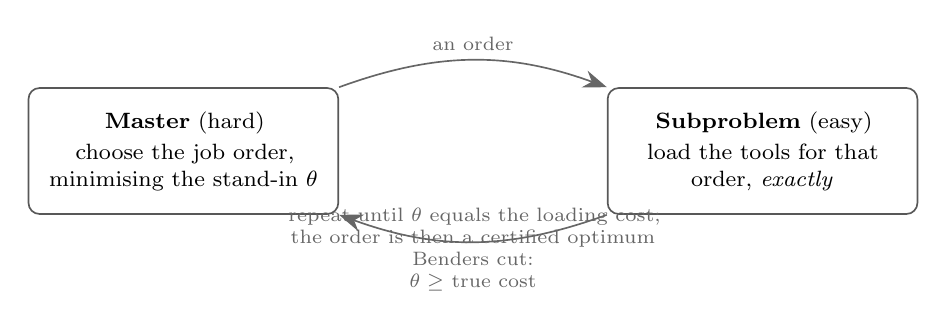
\begin{tikzpicture}[font=\footnotesize,>=Stealth,
   blk/.style={draw,semithick,rounded corners,align=center,minimum height=1.6cm,text width=3.7cm}]
  \node[blk,draw=cBlue!70,fill=white] (m) {\textbf{Master} (hard)\\[2pt] choose the job order,\\ minimising the stand-in $\theta$};
  \node[blk,right=3.4cm of m,draw=cGreen!70,fill=white] (s) {\textbf{Subproblem} (easy)\\[2pt] load the tools for that\\ order, \emph{exactly}};
  \draw[-{Stealth[length=3mm]},semithick,black!60] (m.north east) to[bend left=20] node[above,font=\scriptsize]{an order} (s.north west);
  \draw[-{Stealth[length=3mm]},semithick,black!60] (s.south west) to[bend left=20]
      node[below,align=center,font=\scriptsize]{Benders cut:\\ $\theta\ge$ true cost} (m.south east);
  \node[below=6mm of $(m)!0.5!(s)$,text width=8.6cm,align=center,font=\scriptsize,text=black!60]
     {repeat until $\theta$ equals the loading cost; the order is then a certified optimum};
\end{tikzpicture}
\caption{The branch-and-Benders-cut loop. The master picks an order using an
optimistic stand-in $\theta$ for the loading cost. The subproblem returns the exact
loading cost of that order. If $\theta$ undershot, one cut lifts it, and that cut is
valid for every order, not only the current one. Because the subproblem is polynomial
each cut comes from an exactly solved subproblem, so the loop halts at a proven optimum. The cuts are separated
inside a branch-and-bound tree over the order variables, which is what makes the
method a \emph{branch}-and-Benders-cut.}
\label{fig:benders}
\end{figure}

\paragraph{The master problem.}
Introduce a depot node $d$ with an empty tool requirement, and arc variables
$x_{ij}\in\rset{0,1}$ for $i,j\in J\cup\rset{d}$ with $i\ne j$, where $x_{ij}=1$ means
job $j$ runs immediately after $i$. The depot marks the start and the end, so the
$x$ variables describe a Hamiltonian path through the jobs. The assignment
constraints
\[
  \sum_{i\ne j}x_{ij}=1\ \ (\forall j),\qquad \sum_{j\ne i}x_{ij}=1\ \ (\forall i),
\]
together with subtour-elimination constraints
$\sum_{i,j\in S}x_{ij}\le\lvert S\rvert-1$ for $S\subseteq J$, enforce that. The
master problem is then
\[
  \min\ \theta
\]
subject to the assignment constraints, the subtour constraints, the bound rows
described next, and the Benders cuts generated during the search.

Three families of rows bound $\theta$ from below before any cut is generated.

\emph{The pairwise bound.} At the boundary between consecutive jobs $i$ and $j$ at
least $w_{ij}:=\max(0,\lvert T_i\cup T_j\rvert-b)$ tools are switched, since the
magazine holds $b$ tools but must serve $T_i$ and then $T_j$. This is the bound of
\citet{Tang1988}. Because the subproblem charges insertions from an empty magazine,
the first job also costs at least $\lvert T_{j}\rvert$ insertions, and that term is
carried on the depot arcs. Summing gives the valid inequality
\[
  \theta\ \ge\ \sum_{i,j\in J} w_{ij}\,x_{ij}\;+\;\sum_{j\in J}\lvert T_j\rvert\,x_{d,j},
\]
in which the two contributions are disjoint by position and so may be added.

\emph{The coverage row.} Every tool of $\U$ must be loaded at least once. In the
empty-start cost this gives $\theta\ge\lvert\U\rvert$ directly. This row was absent
from the first implementation, and its absence was the reason the solver performed
poorly in the first campaign; Section~\ref{ssec:validation} records the correction.

\emph{Triplet bounds.} The pairwise argument generalises to ordered triples of jobs,
giving $O(n^{3})$ valid inequalities of the form
$\theta\ge w_{ijk}(x_{ij}+x_{jk}-1)$ with
$w_{ijk}=\max(0,\lvert T_i\cup T_j\cup T_k\rvert-b)$. These are optional and their
effect is measured in Section~\ref{ssec:results-bbc}.

Subtour separation is exact by construction: violated constraints are detected at
integer candidate solutions by a connected-component search, so no optimal solution is
ever removed. Separating them at fractional points would be an acceleration, not a
correctness requirement, and is deliberately absent from the measured configuration.

\paragraph{The subproblem.}
The subproblem must be written in the master's own variables, or the cut it produces
cannot be added to the master. Fix a candidate $\bar{x}$ and introduce, for each job
$j$ and tool $t$, a variable $y_{j,t}\in[0,1]$ for ``tool $t$ occupies the magazine
while job $j$ runs'' and $z_{j,t}\ge0$ counting an insertion of $t$ at $j$. The loading
problem is
\begin{alignat}{3}
  \min\quad & \textstyle\sum_{j}\sum_{t} z_{j,t} \notag\\
  \text{s.t.}\quad
   & y_{j,t}\ \ge\ 1
     &\qquad& t\in T_j &\qquad& [\,\nu_{j,t}\,] \label{eq:sp-req}\\
   & \textstyle\sum_{t} y_{j,t}\ \le\ b
     && \forall j && [\,\mu_j\ge0\,] \label{eq:sp-cap}\\
   & z_{j,t}\ \ge\ y_{j,t}-y_{i,t}-(1-x_{ij})
     && i\ne j,\ \forall t && [\,\lambda_{ijt}\ge0\,] \label{eq:sp-link}\\
   & z_{j,t}\ \ge\ y_{j,t}-(1-x_{dj})
     && \forall j,\ \forall t && [\,\lambda^{d}_{jt}\ge0\,] \label{eq:sp-depot}
\end{alignat}
with $y,z\ge0$. Row~\eqref{eq:sp-link} is the only place the master's variables enter:
when the master selects the arc $(i,j)$, a tool present at $j$ but absent at $i$ must be
inserted at $j$; when it does not, the row is slack. Row~\eqref{eq:sp-depot} does the
same for the first job, charging its whole requirement because the magazine starts
empty. For a fixed $\bar x$ the master's variables appear only on the right-hand side,
so what remains is a linear program in $y$ and $z$ alone; its constraint matrix has the
consecutive-ones property along the path $\bar x$ selects and is therefore totally
unimodular, so the relaxation is integral and, by Proposition~\ref{prop:ktns}, its
optimum equals $\KTNS$ of the order.

\paragraph{The cut, in full.}
Only $\bar x$ appears on the right-hand side of \eqref{eq:sp-link} and
\eqref{eq:sp-depot}, so in the dual it appears only in the objective, and the dual
feasible region does not depend on $\bar x$ at all. Writing the dual explicitly, the
constraint dual to $y_{j,t}$ is
\[
  -\mu_j-\lambda^{d}_{jt}-\sum_{i\ne j}\lambda_{ijt}+\sum_{k\ne j}\lambda_{jkt}
  +\nu_{j,t}\,[\,t\in T_j\,]\ \le\ 0 ,
\]
and the constraint dual to $z_{j,t}$ is
\[
  \lambda^{d}_{jt}+\sum_{i\ne j}\lambda_{ijt}+\eta_{j,t}\,[\,t\notin T_j\,]\ \le\ 1 ,
\]
where $\eta$ prices the non-negativity of $z$ on tools the job does not require and
carries objective coefficient zero, so it never reaches the cut. For any dual-feasible
$(\bar\lambda,\bar\lambda^{d},\bar\mu,\bar\nu)$, weak duality gives the Benders
optimality cut
\begin{equation}\label{eq:benders-cut}
  \theta\ \ge\
  \underbrace{\sum_{i\ne j}\sum_{t}\bar\lambda_{ijt}\,(x_{ij}-1)}_{\text{job-to-job arcs}}
  \;+\;\underbrace{\sum_{j}\sum_{t}\bar\lambda^{d}_{jt}\,(x_{dj}-1)}_{\text{depot arcs}}
  \;-\;b\sum_{j}\bar\mu_j
  \;+\;\sum_{j}\sum_{t\in T_j}\bar\nu_{j,t}.
\end{equation}
Collecting terms, the coefficient of $x_{ij}$ is $\sum_t\bar\lambda_{ijt}$ and every
remaining term is constant, so \eqref{eq:benders-cut} is an affine inequality in the
master's variables and can be added to it verbatim. This is the form the implementation
builds, and it is the form Section~\ref{ssec:disc-locality} analyses when it observes
that every cut the master ever receives is supported on arcs.

Two properties follow immediately. Each cut is a valid lower bound on the loading cost
of \emph{every} order, not only of $\bar x$, because the dual point is feasible for all
of them; it is tight at $\bar x$ when the dual point is optimal there. And because
\eqref{eq:benders-cut} is affine in $x$, its value at a \emph{fractional} $\bar x$ is
defined by the same expression: separating at a fractional master solution means solving
the dual with the fractional $\bar x$ in its objective and adding the resulting affine
row. No reinterpretation of the inequality is required, which is why the fractional
variant of Section~\ref{ssec:accel} needs no separate validity argument.

\begin{remark}[A term whose omission cut off optima]\label{rem:depotterm}
The depot sum in \eqref{eq:benders-cut} is non-positive, so dropping it makes the cut
\emph{tighter} rather than looser, and an implementation that omits it will look
correct on most instances. It was omitted from the first implementation. Because
$\bar\lambda^{d}$ and $\bar\nu$ trade off at zero reduced cost, degenerate dual optima
put positive weight on depot arcs that the order does not use, and the over-tight cut
then removes genuinely optimal $(x,\theta)$ points: $193$ violations were found on
random instances before the term was restored. The campaign reported in
Section~\ref{sec:comp} was run after the correction.
\end{remark}

\subsection{Strengthening the Benders solver}\label{ssec:accel}

Four strengthenings were implemented, each as an independent switch, and each checked
against brute force on small instances before any campaign run so that a strengthening
can never silently return a wrong optimum. All four are classical elements of the
toolbox surveyed by \citet{Rahmaniani2017}.

\paragraph{Fractional Benders cuts.}
The optimality cut is derived at an integer order, but nothing prevents separating the
same cut at the fractional solutions produced at a node before branching. The
intention is to attack tailing-off: an integer-only scheme learns about the loading
cost only once an order is fully committed, whereas a fractional cut extracts the same
dual information from a partial order and removes it from the relaxation at once.

Whether that pays is an empirical question, and Section~\ref{ssec:results-bbc} answers
it.

\paragraph{A strong incumbent at the root.}
A branch-and-bound search prunes in proportion to the quality of its incumbent. A
compact form of the hybrid genetic search of \citet{Mecler2021} is run once, at the
root: a population of constructive seeds, being nearest-neighbour orders on the
pairwise weights $w_{ij}$ and a largest-tool-first order, each improved by a
variable-neighbourhood local search using adjacent swaps and short segment
relocations, with every candidate scored by the exact loading oracle, evolved under
order crossover with a diversity guard.

The resulting order is used twice. As a warm start it gives the solver an incumbent
from node zero. And it seeds a Benders cut: the loading dual is solved once for the
heuristic order and its cut added before the first relaxation, which is the
initial-cut-pool acceleration of \citet{Rahmaniani2017}.

\paragraph{A conflict-graph bound.}
The master's root bound is pairwise plus coverage, and both are visible to the linear
relaxation. The combinatorial structure they miss lives in the conflict graph $G$ of
Section~\ref{ssec:clutter}, whose vertices are the jobs and whose edges join pairs
that cannot share a configuration. A clique of $G$ is a set of pairwise incompatible
jobs, which must occupy that many distinct configurations, so $\Kst\ge\omega(G)$; more
generally $\Kst\ge\chi(G)$, and where $G$ is non-bipartite one has $\chi(G)\ge3$ even
when $\omega(G)=2$. The resulting constant row
$\theta\ge(\chi_{\mathrm{lb}}-1)+\min(b,\lvert\U\rvert)$ is added whenever it strictly
exceeds the coverage row. This is the simplest of the conflict-graph inequalities studied by
\citet{Atamturk2000}. Its reach is narrow by construction: on most instances the
coverage row already dominates it, and it can bite only where the grouping structure,
rather than the tool count, is what forces switches.

\paragraph{Pareto-optimal cut lifting.}
When the loading dual has several optimal solutions, which a degenerate
transportation-type problem routinely does, the cuts they yield are not equally
strong. Choosing the deepest is the Pareto-optimal cut of \citet{MagnantiWong1981}:
among the alternative dual optima, select the one maximising the cut's value at a fixed
interior core point of the master. \citet{Papadakos2008} makes this practical by
observing that the core point need not be tied to the current relaxation and may simply
be updated as a convex combination of the points visited. That form is used here. A
core point is kept in the relative interior of the master polytope, initialised from
the heuristic order blended with the barycentre; at each fractional separation the
loading dual is solved a second time at the core point and its cut added alongside the
ordinary one, after which the core point is drawn halfway towards the current
relaxation point. Adding the core-point cut in addition to, never instead of, the
ordinary cut keeps the scheme valid by construction.

\subsection{Position-indexed formulations}\label{ssec:pos}

The configuration walk of Section~\ref{ssec:gtsp} is the most faithful exact picture
of the SSP, but as a model it has two flaws. There are far too many configurations to
enumerate, and forbidding the subtours that a valid walk must avoid takes exponentially
many constraints.

The position-indexed formulations, proposed by Prof.~Colares, remove both flaws by
fixing the schedule's length in advance. In place of an open-ended walk they lay out a
fixed row of \emph{positions} into which configurations are placed, and ask of each
position which configuration sits there and what it costs to change from the previous
one. Numbering the positions does two useful things at once. It makes the transition
cost a purely local quantity between adjacent slots, so the global subtour constraints
disappear, and it caps the model at a number of rows polynomial in $n$ and
$\lvert T\rvert$. That last property is the point of the construction: the row set is
fixed in advance, so column generation only ever adds columns to rows that already
exist.

\paragraph{Why not Miller--Tucker--Zemlin.}
The obvious alternative is to keep the configuration formulation and replace its
subtour constraints by Miller--Tucker--Zemlin potentials
\citep{Miller1960,DesrochersLaporte1991}. That trades one obstacle for another.

\begin{proposition}\label{prop:mtz}
A potential per configuration is exact but leaves one potential for each of
exponentially many configurations. Aggregating the potentials to one per job is
polynomial but no longer exact: it can exclude the optimum.
\end{proposition}

\begin{proof}
The aggregated form fails under job domination. If $T_i\subseteq T_j$ then every
configuration serving $j$ also serves $i$, so a transition between two such
configurations places both $i$ and $j$ at each of its ends, and the aggregated
potentials of $i$ and $j$ are forced into a two-cycle that no ordering satisfies. A
concrete instance is $b=3$ with $T=(\rset{1,4},\rset{1,3,4},\rset{1},\rset{1,2,4})$,
for which the optimum is $1$ while the aggregated model values it at $2$. This was
verified by exhaustive enumeration over covering paths.
\end{proof}

Neither variant therefore yields a tractable exact model, which is what motivates
fixing the positions instead.

\paragraph{The position--configuration formulation.}
Let $y_C^{k}\in\rset{0,1}$ indicate that configuration $C$ occupies position $k$, for
$k=1,\dots,n$, and let $w_t^{k}\ge0$ count the insertion of tool $t$ at position $k$:
\[
\begin{aligned}
  \min\ & \sum_{t,k} w_t^{k}\\
  \text{(P)}\quad & \sum_{C} y_C^{k}=1, & k&=1,\dots,n;\\
  \text{(Cov)}\quad & \sum_{k}\sum_{C\supseteq T_j} y_C^{k}\ge1, & j&\in J;\\
  \text{(W)}\quad & w_t^{k}\ge\sum_{C\ni t}\bigl(y_C^{k}-y_C^{k-1}\bigr), & t&\in T,\ k\ge2;\\
  \text{(T)}\quad & \sum_{k\ge2} w_t^{k}+\sum_{C\ni t} y_C^{1}\ge1, & t&\in\U.
\end{aligned}
\]
Constraint (P) places one configuration per position, (Cov) serves every job, (W)
charges an insertion whenever a tool enters the magazine, and (T) records that every
used tool is either present at the first position or inserted later. The
configuration variables are generated as columns; the rows number
$O(n\lvert T\rvert)$ and never change. Call this formulation PCF.

\begin{proposition}\label{prop:pcf}
PCF is exact: its integer feasible points are exactly the SSP schedules, with equal
cost. Its linear relaxation \emph{without} the counting rows (T) equals $0$. With
them it equals $q$.
\end{proposition}

The proof is in Appendix~\ref{app:proofs}.

The vanishing of the plain relaxation is the fractional pathology of
\citet{Tang1988} again: a single convex blend of configurations, repeated at every
position, satisfies (P), (Cov) and (W) at zero cost. The counting rows restore the
coverage bound, matching the multicommodity model of
Proposition~\ref{prop:sspmf-lp} with one extra family of rows.

\paragraph{Symmetry reduction.}
PCF carries a large padding symmetry. A schedule using $m<n$ distinct configurations
is encoded by repeating configurations to fill all $n$ positions, and the repeats may
sit anywhere, so one schedule has many equal-cost encodings and therefore many
distinct nodes in a search tree. Removing this freedom means relaxing (P) to an
inequality and forcing the empty positions to a suffix:
\[
  \text{(P$'$)}\quad \sum_{C} y_C^{k}\le1\ \ (\forall k);
  \qquad
  \text{(G)}\quad \sum_{C} y_C^{k+1}\le\sum_{C} y_C^{k}\ \ (k=1,\dots,n-1),
\]
with (Cov), (W) and (T) unchanged. Call this PCF$'$. At an integer point the counts
are non-increasing in $k$, so the used positions form a prefix and the empty ones a
suffix, with the cost-free first configuration at position one. The contiguity rows
(G) are not decorative: without them an interior empty position would make (W) read
the re-entry as a full reload and (T) misattribute the free load.

\begin{proposition}\label{prop:pcfprime}
PCF$'$ is exact, and its linear relaxation equals that of PCF: $q$ with the counting
rows, and $0$ without. It removes symmetric integer encodings but does not strengthen
the bound.
\end{proposition}

The proof is in Appendix~\ref{app:proofs}. The separation of concerns is deliberate:
PCF$'$ attacks symmetry, and only the next formulation attacks the bound.

\paragraph{The position--transition formulation.}
To exceed the coverage bound the formulation indexes \emph{transitions} rather than
positions. Augment the configurations with an absorbing tool-less node, used to pad
schedules that change configuration fewer than $n-1$ times, and let
$z_{C,C'}^{k}\ge0$ be a column for the step from position $k$ to position $k+1$ that
leaves $C$ and enters $C'$. The formulation is
\[
\begin{aligned}
  \min\ & \sum_{k=1}^{n-1}\sum_{(C,C')} d(C,C')\,z_{C,C'}^{k}\\
  \text{(S)}\quad & \sum_{(C,C')} z_{C,C'}^{k}=1, & k&=1,\dots,n-1;\\
  \text{(F)}\quad & \sum_{(C,C'):\,t\in C'} z_{C,C'}^{k}
                    =\sum_{(D,D'):\,t\in D} z_{D,D'}^{k+1}, & t&\in T,\ k=1,\dots,n-2;\\
  \text{(Cov)}\quad & \sum_{k=1}^{n-1}\,\sum_{(C,C'):\,T_j\subseteq C} z_{C,C'}^{k}
                    +\!\!\sum_{(C,C'):\,T_j\subseteq C'} z_{C,C'}^{\,n-1}\ \ge\ 1,
                    & j&\in J.
\end{aligned}
\]
Constraint (S) selects one transition per step. The flow-consistency rows (F) require,
tool by tool, that what enters position $k+1$ at the end of step $k$ is what leaves it
at the start of step $k+1$, so the selected columns describe a single coherent walk.
Constraint (Cov) serves every job at the configuration of some position, either the
tail of a step or the head of the last one. As in PCF the rows number
$O(n\lvert T\rvert)$ and are fixed, while the transition columns are generated. Call
this PTF.

\begin{proposition}\label{prop:ptf}
PTF is exact, and its linear relaxation is at least $q$ and can be strictly greater.
\end{proposition}

The proof is in Appendix~\ref{app:proofs}. The second claim is established by a
witness, not by a general argument, which is why it says \emph{can}.

The witnesses are the three instances of Section~\ref{ssec:results-bnp} on which the
recorded root relaxation exceeds $q$. PTF is therefore the first relaxation in this
family to improve on the elementary bound, and it does so with a fixed, polynomial row
set.

The proposition says the relaxation \emph{can} exceed $q$. It says nothing about how
often, or by how much, and Section~\ref{ssec:results-bnp} finds that on the standard
benchmark the answer to both is: rarely, and by one unit. That leaves the question that
decides whether the construction is worth pursuing.

\begin{problem}\label{prob:ptf-gap}
Is there a family of instances on which the PTF relaxation exceeds the coverage bound
$q$ by an amount that grows without bound? Equivalently: is the excess of PTF over $q$
bounded by a constant?
\end{problem}

\paragraph{Column generation and robust branching.}
Both PCF$'$ and PTF have $O(n\lvert T\rvert)$ rows but exponentially many columns, so
their relaxations are solved by column generation. Branching on a single column
$y_C^{k}$ is ineffective under the position symmetry and forces the pricing problem to
carry a growing list of forbidden columns. The branching used here is instead on the
\emph{presence} variables $a_t^{k}=\sum_{C\ni t}y_C^{k}\in\rset{0,1}$, which already
appear in (W). Fixing $a_t^{k}$ to $0$ or $1$ forbids or forces tool $t$ at position
$k$, which in the pricing problem merely shifts one dual weight and leaves the
oracle's form unchanged. This is a robust branching rule, and it is why the
Ryan--Foster rule of \citet{Ryan1981} is not needed here: that rule exists for
set-partitioning masters whose pricing problems variable branching would destroy, and
this master is not of that kind.

\paragraph{Pricing PCF$'$.}
Let $\alpha_k,\gamma_k\le0$ and $\pi_j,\mu_{t,k},\lambda_t\ge0$ be the duals of
(P$'$), (G), (Cov), (W) and (T). Collecting the coefficient of $y_C^{k}$, which enters
(W) and (T) through $a_t^{k}$, gives the reduced cost
\[
  \bar c(C,k)=\beta_k-\sum_{t\in C}\rho_t^{\,k}-\!\!\sum_{j:\,T_j\subseteq C}\!\!\pi_j,
\]
with
\[
  \rho_t^{\,k}=-\mu_{t,k}\,[k\ge2]\;+\;\mu_{t,k+1}\,[k\le n-1]\;+\;\lambda_t\,[k=1,\ t\in\U],
\]
with $\beta_k$ depending only on the position. For each $k$ the most negative reduced
cost is obtained by maximising the configuration-dependent part,
\[
  \max_{\lvert C\rvert=b}\ \sum_{t\in C}\rho_t^{\,k}
  +\!\!\sum_{j:\,T_j\subseteq C}\!\!\pi_j ,
\]
which is to say: choose $b$ tools so as to collect per-tool rewards plus a bonus for
each job whose \emph{entire} requirement lands inside the chosen set. This is a
Set-Union Knapsack Problem \citep{Goldschmidt1994}, the same class as the
grouping-pricing problem of \citet{Crama1994Column}. The branching dual enters
additively in $\rho_t^{\,k}$, so branching does not change the oracle.

\paragraph{Pricing PTF.}
For PTF a column is an ordered pair $(C,C')$, and its reduced cost contains the
bilinear term $\sum_t[t\in C'\setminus C](1-\lambda_t)$ together with chaining terms on
the tools of $C$ and $C'$. The pricing problem cannot therefore separate into a single
set: it must choose two $b$-subsets at once, with $C\ne C'$. The products
$x'_t(1-x_t)$ are linearised by the McCormick inequalities and the problem is solved as
a mixed-integer program with $2\lvert T\rvert$ binary variables. This heavier pricing
is the algorithmic price of PTF's stronger bound, and the contrast between the two
formulations --- PCF$'$ pairing a weak bound with a cheap single-set oracle, PTF a
stronger bound with a costly coupled-pair oracle --- is the central trade-off of this
section.

\paragraph{Accelerations.}
Four accelerations were implemented as independent switches, mirroring those of
Section~\ref{ssec:accel}. \emph{Heuristic pricing} answers the pricing question first
with a fast greedy subset and calls the exact oracle only to certify that no improving
column remains, so exactness is untouched while the costly oracle is skipped on all but
the final round. \emph{Multiple pricing} returns several negative-reduced-cost columns
per round instead of one. \emph{Warm starting} seeds the initial column pool from a
greedy schedule rather than the trivial one-configuration-per-job pool. \emph{Dual
stabilisation} \citep{Lubbecke2005} smooths successive dual vectors to damp the
oscillation that slows column generation on degenerate masters. None of the four
alters the relaxation value or the optimum.

\paragraph{A prototype not reported here.}
A third piece of implementation, a learned policy for choosing among the Benders
master's admissible cuts, was built during the internship but never measured on an
SSP instance. It is reported in Appendix~\ref{app:rl} and kept out of this section
for that reason; nothing elsewhere in this report rests on it.

%==============================================================================
\section{Computational study}\label{sec:comp}
%==============================================================================

Computation here is how the theory is tested. The quantity the
structural results single out, the coverage bound $q$, is also the root relaxation of
every configuration-based method, so a benchmark that records optima and bounds
measures the theory's central variable directly. The campaign also settles a question
that predates the theory and motivated the Benders solver in the first place: the SSP
has a polynomially solvable loading subproblem, which is the textbook precondition for
Benders decomposition, and whether a decomposition can exploit it against modern
compact models had not been tested.

\paragraph{What the section asks, and in what order.}
Each subsection states the question it answers before the measurement that answers it.
Section~\ref{ssec:bench} fixes the protocol and Section~\ref{ssec:validation} asks
whether the implementations are sound. Section~\ref{ssec:results-solved} asks how far
each method gets; Section~\ref{ssec:results-bbc} whether the difficulty is finding good
solutions or proving them optimal, and whether the standard strengthenings move it;
Section~\ref{ssec:results-tight} what separates the instances a method closes from
those it does not. Section~\ref{ssec:results-bnp} puts the same question to the
branch-and-price prototypes, which report their relaxation value directly and so answer
it without reference to solving times. Section~\ref{sec:disc} then asks why the answer
is what it is.

\subsection{Experimental design}\label{ssec:bench}

\paragraph{Instances.}
The benchmark uses the standard SSP instance families, taken from the collection
assembled by \citet{Otiai2024}: the sets of \citet{Catanzaro2015}, of
\citet{Crama1994}, and four of the sets of \citet{Laporte2004}. Every instance in
every family is run; none is skipped, and no instance is selected on the basis of an
outcome. Table~\ref{tab:families} gives the sizes.

\begin{table}[h]\centering
\footnotesize
\begin{tabular}{@{}lrrrl@{}}
\toprule
Family & Instances & Jobs $n$ & Tools $\lvert T\rvert$ & Source \\
\midrule
Catanzaro & $171$ & $8$--$40$  & $5$--$60$  & \citet{Catanzaro2015} \\
Crama     & $160$ & $10$--$40$ & $10$--$60$ & \citet{Crama1994} \\
Laporte3  & $340$ & $8$        & $15$--$25$ & \citet{Laporte2004} \\
Laporte4  & $330$ & $9$        & $15$--$25$ & \citet{Laporte2004} \\
Laporte5  & $340$ & $15$       & $15$--$25$ & \citet{Laporte2004} \\
Laporte7  & $80$  & $10$--$15$ & $10$--$20$ & \citet{Laporte2004} \\
\midrule
Total     & $1{,}421$ & & & \\
\bottomrule
\end{tabular}
\caption{The instance families. An instance is a matrix together with a magazine
capacity. The Crama collection publishes the same matrices at four different
capacities, so its $40$ matrices give $160$ instances; the same convention is applied
throughout.}
\label{tab:families}
\end{table}

\paragraph{Protocol.}
Every run of the Benders solver and of the compact baselines is given a single uniform
time limit of one hour and $16$ gigabytes of memory. There is no early stopping and no
per-configuration retirement rule. All other solver parameters are left at their
defaults, so that the comparison measures the formulations rather than parameter
tuning. The branch-and-price prototypes are run separately, under a ten-minute limit,
for the reason given in Section~\ref{ssec:results-bnp}.

\paragraph{Hardware and software.}
All runs were executed on the LIMOS SLURM cluster, confined to a homogeneous pool of
identical nodes (AMD EPYC~7452, $2\times32$ cores, $512$\,GB of memory), so that
wall-clock times are comparable across runs. The mixed-integer solver is CPLEX~22.1.1
throughout, pinned to four dedicated threads per run. The branch-and-price prototypes
run single-threaded under PySCIPOpt. The campaign was distributed over $120$ SLURM
array shards and produced $16{,}994$ individual runs.

\paragraph{Configurations.}
Twelve solver configurations were run. Three are the reimplemented compact baselines:
F4 of \citet{Catanzaro2015}, written \texttt{CATZ-F4}; LSS of \citet{Laporte2004}; and
SSPMF of \citet{daSilva2024}. F4 was chosen over the F5 that \citet{Catanzaro2015}
recommend because it is the smaller of the two models that share the F3 relaxation, and
implementing F5 did not fit in the time available. The compact side of this comparison
is therefore weaker than the literature allows, and every statement made from it is
made in that knowledge; Section~\ref{ssec:results-summary} reports what follows, which
is that the baselines win anyway. The remaining nine are the Benders solver, in an ablation
over its cut families and its strengthenings. The naming is as follows:
\texttt{BBC-LP} uses the dual optimality cuts, \texttt{BBC-K} the combinatorial cuts,
\texttt{+T} adds the triplet bounds, \texttt{+F} enables fractional separation,
\texttt{+C} the conflict-graph row, \texttt{+H} the hybrid-genetic incumbent,
\texttt{+P} the Pareto-optimal cut lifting, and \texttt{+ACC} all three strengthenings
together.

\paragraph{The reported quantity.}
The common metric is the empty-start cost of the sequence a method returns, evaluated
by the loading oracle. Each formulation has its own native objective, and two of them
use the free-initial convention, so the native values are not comparable across
methods. The empty-start cost of the returned sequence is defined for every method
regardless of its formulation, and it is what makes the cross-method comparison of
Section~\ref{ssec:validation} meaningful.

\subsection{Validation}\label{ssec:validation}

The implementations were subjected to independent computational checks before any
result was recorded, and again from the results themselves. No amount of such checking
proves correctness; what follows is what was checked and what it found.

\paragraph{Before the campaign.}
Every exact solver was checked against brute-force optima on a bank of small instances,
in every combination of its option flags. The loading oracle itself was verified
against an exact dynamic program over magazine states; the verification described in
Appendix~\ref{app:verify} repeats this on $349{,}872$ instance-and-sequence pairs and
finds no disagreement.

\paragraph{Identifying an instance.}
An instance is identified by the family it comes from, its file name, its number of
jobs, its number of tools, and its magazine capacity. All five are needed. The Crama
collection reuses the same file names at four different capacities, so two runs that
agree on the name can be runs on different instances. Keying on the name alone merges
rows describing different instances and produces apparent disagreements between methods
where none exists. The comparison below uses the full identifier.

\paragraph{Cross-method agreement.}
Of the $1{,}421$ instances, $1{,}115$ were solved to proven optimality by at least one
method and $999$ by at least two. On those $999$ there are $41{,}673$ pairs of methods
that both proved an optimum. \emph{In none of them do the two disagree.} Every pair of
methods that both closed an instance returned a sequence of the same empty-start cost.

\paragraph{The two conventions, measured.}
Proposition~\ref{prop:conv} states that the empty-start and free-initial costs of a
sequence differ by the size of the initial load. The campaign confirms it on real
instances. The SSPMF model reports the free-initial cost natively, and on all
$1{,}038$ instances it closed, the difference between its reported value and the
empty-start cost of the same sequence equals the magazine capacity $b$ on $1{,}029$ of
them. On the other nine it is smaller than $b$, and those are exactly the instances on
which an optimal sequence begins with a job that needs fewer than $b$ tools, so the
magazine is not filled at the start. The two baselines that report the empty-start cost
natively, \texttt{CATZ-F4} and LSS, show a difference of zero on all $1{,}729$ runs in
which they closed an instance.

\paragraph{Tools that no job needs.}
Four matrices in the collection contain a tool that appears in no job's requirement
set: Crama \texttt{s2n007} and \texttt{s2n009}, Laporte3 \texttt{L28-7} and Laporte5
\texttt{L6-8}. Counted with the capacities at which they appear, that is ten of the
$1{,}421$ instances. The coverage bound of Corollary~\ref{cor:lb} must therefore be read as
$q=\lvert\U\rvert-b$, using the set $\U$ of tools that some job actually requires, and
not as $\lvert T\rvert-b$ using the tool count declared in the instance file. On those
ten the two differ, and the smaller value is the correct one: on Laporte3
instance \texttt{L28-7}, which declares $25$ tools of which one is never required and
has $b=5$, the optimum in the free-initial convention is $19$, which is
$\lvert\U\rvert-b=24-5$ and not $\lvert T\rvert-b=20$. All coverage-bound figures in
this section use $\lvert\U\rvert$.

\paragraph{A defect found and corrected.}
The Benders master carries the coverage row $\theta\ge\lvert\U\rvert$ of
Section~\ref{ssec:bbc} as an explicit constraint. It has to: unlike every other method
here, the master has no formulation of the loading problem from which that bound would
follow, so without the row it is not available to the relaxation at all.
Observation~\ref{obs:rootq} shows how much work the row does --- on $87.4\%$ of runs the
root relaxation is exactly $\lvert\U\rvert$ and nothing else contributes.

\paragraph{Runs that failed.}
Of the $16{,}994$ runs, $427$ returned no result. Forty-nine are a failure of the
harness itself while closing its log file on the cluster filesystem, and the remaining
$378$ are crashes of the worker subprocess. They are not spread evenly: $352$ of the
crashes belong to the LSS baseline, $239$ of those to the Laporte5 family.

The two groups have different causes, and one of them is recorded.

\emph{The Benders failures.} Of the $75$ failures scattered across the nine Benders
configurations, at most $26$ in any one, $49$ carry an explicit exception:
\texttt{OSError: [Errno 127] Key has expired}. That is expiry of the job's filesystem
credentials on a cluster whose home directories are served over an authenticated mount.
The run lost the ability to write its own output; nothing about the instance or the
solver is implicated. These are infrastructure losses, and they change no comparison
drawn between configurations.

\emph{The LSS crashes.} The remaining $352$ are recorded as
\texttt{subprocess crash} with an empty message: the worker was terminated without
raising, so no exception was captured and the proximate cause is not in the result
files. What the timing shows is that they are not startup failures and not a bad node.
No crash occurs before $1{,}063$ seconds; the median is $2{,}069$ and the maximum
$3{,}582$, just inside the limit. They are distributed evenly over the ten shards, at
between $32$ and $38$ each, so no single node or batch accounts for them. And $239$ of
the $352$ are Laporte5.

A run that survives at least eighteen minutes and is then killed without raising is
consistent with a resource limit reached during the search rather than a defect in the
model, but the campaign does not record enough to establish that: it would take the
scheduler's accounting record for the job, which is not part of the result files. The
obvious size explanation is separately excluded --- measured by $n\lvert T\rvert$ the
crashed runs are \emph{smaller} than the completed ones, median $400$ against $500$.

What is established either way is that the loss is not random with respect to
difficulty. On the instances LSS completed, SSPMF proves optimality $78\%$ of the time;
on the $352$ it lost, only $60\%$. The instances LSS never attempted are the harder
ones, so its totals are flattering and its rate is not comparable with the others.
Section~\ref{ssec:limits} records what follows from that.

\subsection{How far each method gets}\label{ssec:results-solved}

\emph{The question.} How many instances does each method close, and does the
decomposition compete with the compact models it was built to improve on?

This is the coarsest measurement in the section and the least explanatory. It
establishes a ranking, and that ranking is the starting point for everything after it,
but by itself it says nothing about \emph{why} the ranking is what it is.
Sections~\ref{ssec:results-bbc} and \ref{ssec:results-tight} take that up.

Table~\ref{tab:solves} reports, for each configuration and each family, the number of
instances solved to proven optimality against the number of runs that returned a
result.

\begin{table}[t]\centering
\scriptsize
\setlength{\tabcolsep}{4pt}
\begin{tabular}{@{}lrrrrrrr@{}}
\toprule
Configuration & Catanzaro & Crama & Laporte3 & Laporte4 & Laporte5 & Laporte7 & All\\
\midrule
SSPMF              & $73/171$ & $68/160$ & $340/340$ & $330/330$ & $161/336$ & $66/80$ & $1038/1417$\\
\texttt{CATZ-F4}   & $55/171$ & $44/160$ & $340/340$ & $330/330$ & $72/327$  & $44/78$ & $885/1406$\\
LSS                & $52/132$ & $42/124$ & $340/340$ & $330/330$ & $39/101$  & $41/42$ & $844/1069$\\
\midrule
\texttt{BBC-LP+T}  & $38/168$ & $34/156$ & $340/340$ & $192/330$ & $84/336$  & $39/80$ & $727/1410$\\
\texttt{BBC-LP}    & $38/169$ & $35/151$ & $340/340$ & $191/329$ & $83/338$  & $39/80$ & $726/1407$\\
\texttt{BBC-K}     & $39/166$ & $34/145$ & $340/340$ & $190/329$ & $83/335$  & $39/80$ & $725/1395$\\
\texttt{BBC-LP+F+H}& $43/171$ & $37/160$ & $316/340$ & $157/330$ & $97/339$  & $40/80$ & $690/1420$\\
\texttt{BBC-LP+F}  & $37/169$ & $32/160$ & $313/340$ & $156/329$ & $85/340$  & $36/80$ & $659/1418$\\
\texttt{BBC-LP+F+C}& $37/170$ & $32/160$ & $311/340$ & $157/329$ & $84/336$  & $36/79$ & $657/1414$\\
\texttt{BBC-LP+ACC}& $43/170$ & $37/160$ & $286/340$ & $154/330$ & $97/339$  & $39/80$ & $656/1419$\\
\texttt{BBC-K+F}   & $37/171$ & $21/121$ & $316/340$ & $156/329$ & $86/338$  & $35/79$ & $651/1378$\\
\texttt{BBC-LP+F+P}& $35/171$ & $32/160$ & $282/340$ & $155/328$ & $83/336$  & $35/79$ & $622/1414$\\
\bottomrule
\end{tabular}
\caption{Instances solved to proven optimality, against runs that returned a result,
under a one-hour limit. Denominators below the family size are the failed runs of
Section~\ref{ssec:validation}; the LSS row is the one where this matters, and its
totals should not be read against the others.}
\label{tab:solves}
\end{table}

Three things can be read from Table~\ref{tab:solves}.

The compact models dominate the decomposition. SSPMF closes $1{,}038$ instances against
$727$ for the best Benders configuration, and that gap is far larger than anything the
missing runs could account for.

Among the compact models themselves the ranking is less clear than the totals suggest,
because LSS did not complete a third of its runs. On the $1{,}067$ instances that LSS
and SSPMF both attempted, LSS proves $844$ optima and SSPMF $827$; on the $1{,}066$
that LSS and \texttt{CATZ-F4} both attempted, \texttt{CATZ-F4} proves $865$ against LSS's
$844$. Since the runs LSS lost are the harder ones, its position in both comparisons is
flattered by an unknown amount. The honest reading is that the three compact models are
close to one another on this collection and that separating them would need the lost
runs recovered; what the campaign does establish is that all three are ahead of the
methods built here.

The families separate the methods rather than rank them uniformly. Laporte3 is solved
completely by six of the twelve configurations. Laporte4 splits them sharply: the
three compact models solve all $330$, and the Benders solver solves between $154$ and
$192$. Catanzaro and Crama are hard for everything, and no method closes more than
half of either.

Among the Benders variants, the three that do not separate at fractional points
(\texttt{BBC-LP}, \texttt{BBC-LP+T}, \texttt{BBC-K}) are the three best, within two
instances of one another. Every configuration carrying \texttt{+F} is worse than all
three. Section~\ref{ssec:results-bbc} takes that apart.

\paragraph{Solving times.}
Table~\ref{tab:times} reports times on the $535$ instances that all eight of the listed
configurations solve. The shifted geometric mean with a shift of ten seconds is used,
following standard practice for exact-method comparisons, because it is insensitive to
both very small and very large individual values.

\begin{table}[h]\centering
\footnotesize
\begin{tabular}{@{}lrrr@{}}
\toprule
Method & shifted geometric mean (s) & median (s) & maximum (s)\\
\midrule
SSPMF              & $1.90$  & $0.140$  & $48.7$\\
\texttt{BBC-K}     & $14.50$ & $0.018$  & $845.8$\\
\texttt{BBC-LP+T}  & $16.03$ & $0.066$  & $1126.0$\\
\texttt{BBC-LP}    & $16.11$ & $0.067$  & $1128.4$\\
\texttt{BBC-LP+F+H}& $30.74$ & $0.003$  & $3584.6$\\
\texttt{BBC-LP+F}  & $33.73$ & $0.107$  & $3586.6$\\
LSS                & $37.68$ & $18.254$ & $2211.5$\\
\texttt{CATZ-F4}   & $92.83$ & $74.304$ & $3506.5$\\
\bottomrule
\end{tabular}
\caption{Solving times on the $535$ instances that all eight configurations solve. The
Benders solver has by far the lowest median and a high mean, which is the signature of
a method that either finishes almost at once or struggles.}
\label{tab:times}
\end{table}

The pattern in Table~\ref{tab:times} is as informative as the ranking. The Benders
solver's median is one to three orders of magnitude below every compact model's, while
its mean is an order of magnitude above SSPMF's. It either closes an instance
immediately or does not close it at all. Section~\ref{ssec:results-tight} identifies
what separates the two cases, and it is not the size of the instance that does so.

\paragraph{How the solved count accumulates.}
The shifted geometric mean summarises the instances a method solves; it says nothing
about the ones it does not. Table~\ref{tab:cumulative} gives the whole curve: how many
instances each method has closed by one second, ten seconds, and so on to the limit.

\begin{table}[h]\centering
\footnotesize
\begin{tabular}{@{}lrrrrrrr@{}}
\toprule
Method & $1$s & $10$s & $60$s & $300$s & $900$s & $3600$s & attempted\\
\midrule
SSPMF              & $482$ & $735$ & $946$ & $959$ & $982$ & $1038$ & $1417$\\
\texttt{CATZ-F4}   & $128$ & $254$ & $444$ & $662$ & $795$ & $885$  & $1406$\\
LSS                & $57$  & $246$ & $532$ & $759$ & $819$ & $844$  & $1069$\\
\midrule
\texttt{BBC-LP}    & $403$ & $469$ & $525$ & $572$ & $650$ & $726$  & $1407$\\
\texttt{BBC-K}     & $431$ & $490$ & $531$ & $570$ & $699$ & $725$  & $1395$\\
\texttt{BBC-LP+F}  & $362$ & $435$ & $466$ & $508$ & $542$ & $659$  & $1418$\\
\bottomrule
\end{tabular}
\caption{Instances closed within a given time. The two groups have different shapes.}
\label{tab:cumulative}
\end{table}

\begin{figure}[h]\centering
\begin{tikzpicture}
\begin{semilogxaxis}[reportaxis, width=0.95\linewidth, height=6.6cm,
  xlabel={wall-clock time (seconds, log scale)}, ylabel={instances closed},
  xmin=0.05, xmax=3600, ymin=0, ymax=1120,
  xtick={0.1,1,10,60,300,3600},
  xticklabels={$0.1$,$1$,$10$,$60$,$300$,$3600$},
  ytick={0,200,400,600,800,1000},
  yticklabel style={/pgf/number format/fixed,/pgf/number format/1000 sep={,}},
  legend pos=south east, legend columns=2, transpose legend]
  \addplot[black,    no marks]                  table[x=t,y=SSPMF]   {figdata/cactus.dat}; \addlegendentry{SSPMF}
  \addplot[black,    no marks, dashed]          table[x=t,y=CATZF4]  {figdata/cactus.dat}; \addlegendentry{\texttt{CATZ-F4}}
  \addplot[black,    no marks, dotted]          table[x=t,y=LSS]     {figdata/cactus.dat}; \addlegendentry{LSS}
  \addplot[black!55, no marks]                  table[x=t,y=BBCLP]   {figdata/cactus.dat}; \addlegendentry{\texttt{BBC-LP}}
  \addplot[black!55, no marks, dashed]          table[x=t,y=BBCK]    {figdata/cactus.dat}; \addlegendentry{\texttt{BBC-K}}
  \addplot[black!55, no marks, dotted]          table[x=t,y=BBCLPpF] {figdata/cactus.dat}; \addlegendentry{\texttt{BBC-LP+F}}
\end{semilogxaxis}
\end{tikzpicture}
\caption{Every solved run in the campaign, not the six sampled columns of
Table~\ref{tab:cumulative}: for each method, the number of instances closed by each
wall-clock time. The curves cross, and where they cross is what matters here. Before about
two seconds the configurations built here lead the field --- \texttt{BBC-K} has a
median solve time of $0.06$ seconds against $59.8$ for \texttt{CATZ-F4} --- because a
Benders master with a tight coverage row closes an instance at the root immediately or
not at all. After two seconds they stop moving and every compact model overtakes them.
The decomposition is not running out of time. It has stopped making progress, and what
would restart it is a bound that improves when the solver branches.}
\label{fig:cactus}
\end{figure}

The shapes differ, and the difference is the point. \texttt{BBC-LP} closes $403$
instances in the first second and $726$ in the full hour: more than half of everything
it will ever solve is solved before a compact model has finished building its model.
After that it flattens. SSPMF starts lower relative to its own total, at $482$ of
$1{,}038$, and keeps climbing throughout; LSS closes $57$ in the first second and
$844$ by the end. Extending the limit would therefore not affect the methods equally.
The Benders solver is not slow. It is fast on one class of instance and unable to
finish on the other, which is the behaviour Section~\ref{ssec:results-tight} explains.

\paragraph{How far from proven the unsolved runs are.}
The complement of the solved count is the gap remaining when the limit is reached,
measured between the incumbent and the dual bound. For \texttt{BBC-LP} the median over
its $681$ time-limited runs is $22.9\%$ and the mean is $28.6\%$, with a maximum of
$73\%$; the nine Benders configurations lie between $26.0\%$ and $29.5\%$ on the mean.
Only $50$ of those $681$ runs finish within five per cent of proven.

That figure should be read against the one in the next paragraph. On the runs where the
optimum is known independently, the solver's incumbent already equals it $59\%$ of the
time. It is therefore sitting on the right answer with a certified gap of roughly a
quarter, and the hour is spent failing to close a gap that exists only in the
certificate.

\subsection{The Benders solver and its strengthenings}\label{ssec:results-bbc}

\emph{The question.} A branch-and-bound method can fail for two reasons: it cannot find
a good solution, or it finds one and cannot prove it optimal. The two call for opposite
remedies, and the ablation below is designed to tell them apart. Four strengthenings
were implemented, one aimed at the incumbent and three at the dual bound. If the
difficulty is search, the first should be marginal and the others should help. If the
difficulty is the bound, the pattern should be reversed.

That is what makes this subsection informative rather than merely a list of settings:
the outcome discriminates between two explanations, and it was not obvious in advance
which one it would pick.

\paragraph{Fractional cuts.}
Separating Benders cuts at fractional points is a standard acceleration whose value on
this problem had not been established. The measurement below settles it.

The cuts are now generated in very large numbers. Across the $1{,}415$ instances that
both \texttt{BBC-LP} and \texttt{BBC-LP+F} attempted, the fractional configuration
added $67{,}513{,}396$ cuts, and the configuration without fractional separation added
none, which is the expected control.

They do not help. Table~\ref{tab:frac} gives the comparison.

\begin{table}[h]\centering
\footnotesize
\begin{tabular}{@{}lrr@{}}
\toprule
On the $1{,}415$ common instances & \texttt{BBC-LP} & \texttt{BBC-LP+F}\\
\midrule
fractional cuts added        & $0$   & $67{,}513{,}396$\\
solved to optimality         & $726$ & $659$\\
median nodes explored        & $77{,}504$ & $3{,}795$\\
\midrule
\multicolumn{3}{@{}l}{final dual bound, on the $1{,}404$ instances where both are recorded:}\\
\quad strictly higher with fractional cuts & \multicolumn{2}{r}{$0$}\\
\quad equal                                & \multicolumn{2}{r}{$1{,}228$}\\
\quad strictly lower with fractional cuts  & \multicolumn{2}{r}{$176$}\\
\bottomrule
\end{tabular}
\caption{The effect of enabling fractional Benders cuts. Sixty-seven million cuts
enter the master. The bound at termination is never higher than without them, and on
$176$ instances it is lower. The node counts are consistent with the hour going into
generating and managing cuts instead of searching, though the campaign does not isolate
that mechanism. Sixty-seven instances that the base solver closes are lost.}
\label{tab:frac}
\end{table}

The mechanism works:
the cuts are valid, they are generated, and they enter the master. The node counts show
they do tighten the relaxation locally, since the search explores twenty times fewer
nodes. What they do not do is raise the bound that matters. On no instance in the
comparison is the bound at termination higher with them than without.

The reading is that the fractional dual information is not new information. The
integer cuts already give the master everything the loading dual has to say, and the
fractional ones re-derive it at a cost of an hour of separation.

\paragraph{The three strengthenings.}
Table~\ref{tab:ablation} compares each strengthening against \texttt{BBC-LP+F} on the
instances both attempted.

\begin{table}[h]\centering
\footnotesize
\begin{tabular}{@{}llrrr@{}}
\toprule
Configuration & what it adds & common & solved & difference\\
\midrule
\texttt{BBC-LP+F}   & ---                        & ---       & ---   & ---\\
\texttt{BBC-LP+F+H} & hybrid-genetic incumbent   & $1{,}421$ & $690$ & $+31$\\
\texttt{BBC-LP+F+C} & conflict-graph row         & $1{,}421$ & $657$ & $-2$\\
\texttt{BBC-LP+ACC} & all three together         & $1{,}421$ & $656$ & $-3$\\
\texttt{BBC-LP+F+P} & Pareto-optimal cut lifting & $1{,}421$ & $622$ & $-37$\\
\midrule
\texttt{BBC-LP}     & fractional separation removed & $1{,}415$ & $726$ & $+67$\\
\bottomrule
\end{tabular}
\caption{Each strengthening against \texttt{BBC-LP+F}, on the instances both attempted.
Only the one that improves the incumbent helps. The two that aim at the dual bound
cost more time than they return, and combining all three does not recover the loss.
The last row is the comparison of Table~\ref{tab:frac}, repeated here because removing
a feature outperforms every addition.}
\label{tab:ablation}
\end{table}

The pattern is consistent and it is the same pattern as the fractional cuts. The only
strengthening that helps is the one that supplies a better \emph{incumbent}. Every
attempt to improve the \emph{bound} costs more than it returns. The conflict-graph row
is neutral, which is what Section~\ref{ssec:accel} predicted for it on structural
grounds: on most instances the coverage row already dominates it.

\paragraph{Where the search stops.}
Two further measurements locate the difficulty precisely.

First, of the $726$ instances \texttt{BBC-LP} solves, $259$ are closed at the root
node, without branching at all. The root relaxation value was recorded on $1{,}178$ of
the $1{,}421$ runs, and on $883$ of those the optimum is also known. On those $883$ the
root value equals the optimum $294$ times, and the split is sharp: among the runs that
went on to close the instance it is already the optimum in $264$ of $497$, and among
the runs that did not close it in only $30$ of $386$. Where it is not the optimum it is
short of it by at least one unit and by $16.7\%$ at the median, rising to $42.9\%$.

Second, consider the runs that hit the time limit. Across the nine Benders
configurations there are $6{,}562$ of them, and for $3{,}874$ the optimum is known
because some method proved it. On $2{,}571$ of those $3{,}874$, which is $66\%$, the
Benders solver's incumbent already \emph{equals} that optimum. It had found the answer
and could not prove it. For \texttt{BBC-LP} alone the figure is $229$ of $386$, or
$59\%$.

Taken together these two measurements describe a solver that finishes at the root when
the bound is good, and that finds the optimum quickly and then spends an hour failing to
certify it when the bound is bad. In neither case is the search the constraint on what
it can do.

\subsection{The coverage bound decides the outcome}\label{ssec:results-tight}

Section~\ref{sec:gap} predicted that the coverage bound $q$ would separate easy
instances from hard ones for any configuration-based method. That prediction is
directly testable, because for each instance with a known optimum it can be checked
whether the optimum equals the bound.

Of the $1{,}115$ instances whose optimum is known, $523$ have the coverage bound tight
and $592$ do not. The split is close to even, at $46.9\%$ tight, which means the
standard instance collections are not concentrated in either regime. Where the bound is
loose it is loose by a wide margin: the optimum exceeds it by $5.71$ on average and by
as much as $30$.

Splitting the results by that criterion gives Table~\ref{tab:tightness}.

\begin{table}[h]\centering
\footnotesize
\begin{tabular}{@{}lrrrr@{}}
\toprule
& instances & \texttt{BBC-LP} solves & SSPMF solves\\
\midrule
coverage bound tight ($\Zst=q$)  & $523$ & $492$ \; ($94\%$) & $523$ \; ($100\%$)\\
coverage bound loose ($\Zst>q$)  & $592$ & $234$ \; ($40\%$) & $515$ \; ($87\%$)\\
\bottomrule
\end{tabular}
\caption{Success rate split by whether the coverage bound equals the optimum. The
bound, rather than the size of the instance, is what the outcome tracks for the
Benders solver. The multicommodity model is affected by the same split but far less. A natural
reading is that a compact model gives its search a full description of the problem at
every node, so the search recovers what the bound does not supply; the campaign shows the
difference but does not test that explanation.}
\label{tab:tightness}
\end{table}

\begin{figure}[h]\centering
\begin{tikzpicture}
\begin{axis}[reportaxis, height=6.2cm,
  xlabel={how loose the coverage bound is on the instance \ (\,$\Zst-q$\,)},
  ylabel={instances closed (\%)},
  xmin=-0.6, xmax=8.6, ymin=0, ymax=112,
  xtick={0,1,2,3,4,5,6,7,8},
  xticklabels={$0$,$1$,$2$,$3$,$4$,$5$--$6$,$7$--$9$,$10$--$14$,$15+$},
  ytick={0,20,40,60,80,100},
  legend style={at={(0.03,0.06)}, anchor=south west}]
  \addplot[black, mark=*, mark size=1.9]
    coordinates {(0,100.0)(1,100.0)(2,100.0)(3,100.0)(4,100.0)(5,96.6)(6,84.3)(7,63.9)(8,9.3)};
  \addlegendentry{SSPMF (compact)}
  \addplot[black!55, mark=o, mark size=1.9, dashed]
    coordinates {(0,94.1)(1,30.4)(2,37.8)(3,42.9)(4,60.7)(5,34.1)(6,47.0)(7,52.5)(8,9.3)};
  \addlegendentry{\texttt{BBC-LP} (this report)}
  \node[font=\scriptsize, text=black!55, anchor=west] at (axis cs:0.15,104) {$523$ instances};
  \node[font=\scriptsize, text=black!55, anchor=east] at (axis cs:7.85,15) {$43$ instances};
\end{axis}
\end{tikzpicture}
\caption{The $1{,}115$ instances of known optimum, grouped by how far the optimum
exceeds the coverage bound, against the share each method closes. This is
Table~\ref{tab:tightness} resolved into its whole response curve, and the curve says
more than the two-way split does. The Benders solver does not degrade: it falls off a
cliff between a bound that is exact and a bound that is wrong by one, from $94\%$ to
$30\%$, and then wanders without trend --- once the bound is loose at all, by how much
stops mattering. The compact model degrades smoothly instead, holding $100\%$ out to a
gap of four. But the two meet again at the right-hand end: on the $43$ instances whose
bound is loose by fifteen or more, \emph{both} close $9.3\%$. The compact model is not
immune to the bound; it has further to fall.}
\label{fig:tightsplit}
\end{figure}

This is the central measurement of the campaign. The same solver, on the same hardware,
under the same time limit, closes $94\%$ of one class and $40\%$ of the other. The
classification is not by number of jobs, number of tools or density; it is by a single
structural property of the instance, and it is the property the theory of
Section~\ref{sec:gap} identifies.

The SSPMF column is the useful control. Its relaxation is also equal to $q$, so if the
bound were the whole story it should show the same collapse. It does not: it falls from
$100\%$ to $87\%$ where the Benders solver falls from $94\%$ to $40\%$. A compact model
gives the branch-and-bound search a full description of the problem to work with at
every node, and the search recovers much of what the bound does not supply. The Benders
master sees only the cuts it has accumulated, and when the bound is loose it has very
little else.

\subsection{Branch-and-price: the relaxation measured directly}\label{ssec:results-bnp}

\emph{The question.} Everything above measures the bound indirectly, through how many
instances a solver closes. The prototypes can answer directly, because they report the
value of their root relaxation on every run. Two propositions of Section~\ref{ssec:pos}
predict what that value will be --- that PCF$'$ equals the coverage bound and that PTF
can exceed it --- and the campaign is a chance to test a proof against a benchmark
rather than against another proof.

That is the whole purpose of this run, and it is worth being explicit about what it is
not. It is not a fourth entry in the comparison of Section~\ref{ssec:results-solved}.
The prototypes are implemented in Python over PySCIPOpt with a Python pricer, so a
single node costs orders of magnitude more than a node of a compiled solver; their
wall-clock times measure the implementation language, not the formulation, and are
never compared against CPLEX anywhere in this report. The quantity this subsection
exists to report is the root relaxation value, which is a property of the formulation
and is recorded before any search happens. The solve counts are given because a
reader will ask for them, and are read only as evidence that the prototypes are
working code.

In total $2{,}581$ runs were made over $469$ instances in seven
configurations: PCF$'$ alone; PCF$'$ with each of the four accelerations of
Section~\ref{ssec:pos} separately, written \texttt{+HP} for heuristic pricing,
\texttt{+MC} for multiple pricing, \texttt{+WS} for warm starting and \texttt{+STAB}
for dual stabilisation; PCF$'$ with all four together, written \texttt{+ACC}; and PTF.
The time limit is thirty minutes on the Catanzaro and Crama families and ten minutes on
the Laporte families.

Two properties of this run make its counts weaker still, and both are stated before the
numbers. First, the harness carries an early-stop rule: once a configuration has failed
to close six increasingly hard instances in succession, the remaining harder instances
are skipped for that configuration. The number of runs a configuration received
therefore depends on how it performed, so the denominators in Table~\ref{tab:bnp} are
not comparable across rows. Second, no repetition or seed variation was run. Every
comparison drawn below is made either on instances that both configurations attempted,
or on the root relaxation value, which the early-stop rule cannot bias because it is
recorded before any search.

\paragraph{They agree with the campaign.}
On the $507$ runs that proved an optimum and where the same instance was also closed in
the campaign of Section~\ref{ssec:results-solved}, the two agree on every one. As in
Section~\ref{ssec:validation}, the native objective is the free-initial cost and the
difference from the empty-start cost is exactly $b$ on all $507$.

\paragraph{What the root relaxation shows.}
Proposition~\ref{prop:pcf} states that the position--configuration relaxation equals
the coverage bound $q$, and Proposition~\ref{prop:ptf} states that the
position--transition relaxation can exceed it. Both are testable directly, because the
prototypes record the root relaxation value.

\emph{PCF$'$ never exceeds $q$.} On all $2{,}114$ PCF$'$ runs for which a root
relaxation value was recorded, that value equals $\lvert\U\rvert-b$ exactly. Not one
run, in any of the six PCF$'$ configurations, produced a root bound above the counting
bound. This is Proposition~\ref{prop:pcf} confirmed on the benchmark rather than on
paper.

\emph{PTF exceeds $q$, and almost never.} Of the $233$ PTF runs with a recorded root
relaxation, three are strictly above $\lvert\U\rvert-b$: Catanzaro \texttt{A0-0}, where
the bound is $2.013$ against $q=2$, and Laporte3 \texttt{L11-6} and \texttt{L11-7},
where it is $6$ against $q=5$. Proposition~\ref{prop:ptf} is therefore not vacuous. But
$230$ of $233$ runs sit exactly on $q$, and on the two Laporte3 instances the optima
are $12$ and $13$, so a bound of $6$ instead of $5$ closes a small part of a large gap.

\emph{The bound is often already the answer.} On $990$ of the $1{,}846$ runs where both
the root relaxation and the optimum are known, the root relaxation \emph{equals} the
optimum. These are the tight instances of Section~\ref{ssec:results-tight}, seen from
the other side: where the coverage bound is tight, a configuration-based relaxation
needs no strengthening at all, and where it is loose, neither PCF$'$ nor PTF supplies
one.

\paragraph{What the prototypes close, and why that is not the measurement.}
Table~\ref{tab:bnp} gives the counts, for completeness rather than for comparison.
Nothing above nine jobs was closed by any configuration: all $608$ runs on the $30$-job
and $40$-job instances reached the time limit. This is the expected consequence of a
Python pricer and is not evidence about the formulation, which the paragraph above has
already measured.

\begin{table}[h]\centering
\footnotesize
\begin{tabular}{@{}llrrrr@{}}
\toprule
Configuration & what it adds & runs & solved & median time (s) & median columns\\
\midrule
PCF$'$\texttt{+MC}   & multiple pricing          & $422$ & $102$ & $11.4$ & $1{,}504$\\
PCF$'$               & ---                       & $415$ & $91$  & $23.7$ & $1{,}574$\\
PCF$'$\texttt{+HP}   & heuristic pricing         & $360$ & $73$  & $19.7$ & $5{,}173$\\
PTF                  & position--transition rows & $387$ & $73$  & $2.4$  & $1{,}279$\\
PCF$'$\texttt{+WS}   & warm-started pool         & $359$ & $64$  & $14.9$ & $1{,}610$\\
PCF$'$\texttt{+ACC}  & all four together         & $337$ & $60$  & $28.1$ & $1{,}221$\\
PCF$'$\texttt{+STAB} & dual stabilisation        & $301$ & $44$  & $35.7$ & $1{,}133$\\
\bottomrule
\end{tabular}
\caption{The branch-and-price prototypes, reported as evidence that the code runs and
not as a performance comparison. Median time is over the runs that closed; median
columns is over all runs. The run counts are outcome-dependent through the early-stop
rule, so the rows are not comparable with one another, and none of them is comparable
with the compiled solvers of Table~\ref{tab:solves}. The measurement this subsection
exists for is the root relaxation above.}
\label{tab:bnp}
\end{table}

Head to head on the $320$ instances both attempted, PCF$'$ and PTF each close $73$.
Their node counts differ by a factor of fifty --- a median of $96$ against $2$ ---
because the PTF pricer prices coupled pairs of configurations and costs far more per
node. The stronger relaxation does not convert into more instances closed.

\paragraph{The comparison with the Job Grouping Problem.}
\citet{Otiai2024} builds a branch-and-price for that problem whose set-covering
relaxation is strong enough to close benchmark instances in a handful of nodes. For the
SSP, \citet{Moreira2026} reports that the trivial bound $\lvert T\rvert-b$ obtained by
the multicommodity model was the best available bound on all thirty instances of three
of his subgroups, with the configuration model giving the best bound on four instances
of the remaining, tighter subgroup. The measurements above say the same thing on a
larger collection and with the mechanism visible: the configuration relaxation for the
SSP is not, in general, an improvement on the counting bound.

\subsection{What the campaign establishes}\label{ssec:results-summary}

Two of the results above are checks that the study is sound. Cross-method agreement is
complete: on the $999$ instances solved by more than one method, all $41{,}673$ pairs
agree on the cost of the schedule returned. And the three reimplemented compact models
all close substantially more instances than any configuration built here, without being
cleanly separable from one another, because the LSS runs that failed are the harder
ones.

The remaining four converge on one statement. Whether the coverage bound equals the
optimum decides whether the Benders solver closes an instance, and where it fails the
incumbent is usually already optimal. Of four strengthenings, only the one that
improves the incumbent helps; the three aimed at the bound are neutral or harmful, and
the sixty-seven million fractional cuts are the extreme case, raising the bound at
termination on no instance while costing sixty-seven solved ones. Both branch-and-price
relaxations sit on the coverage bound or barely above it, confirming
Propositions~\ref{prop:pcf} and \ref{prop:ptf} and showing the second to be of little
practical use as it stands. Section~\ref{sec:disc} takes that up.

%==============================================================================
\section{Discussion}\label{sec:disc}
%==============================================================================

\subsection{Bound-limited, not implementation-limited}\label{ssec:disc-bound}

A method can fail to solve an instance for two reasons. It can fail to find a good
solution, or it can find one and fail to prove that no better one exists. The
distinction matters because the two failures call for different remedies. The first
is answered by better search: heuristics, warm starts, branching rules. The second is
answered only by a better bound.

For the SSP the campaign answers this question unambiguously, and it answers it four
times over.

The first answer is in the direct measurement. On the runs that hit the time limit and
whose optimum is known from elsewhere, the Benders solver's incumbent already equals
that optimum $66\%$ of the time across its nine configurations, and $59\%$ of the time
for the plain one. In those runs the solver has already found the answer and spends the
remaining hour failing to certify it.

The second answer is in the ablation. Four strengthenings were implemented. The one
that improves the incumbent, a hybrid genetic search run at the root, gains thirty-one
instances. The three that aim at the dual bound --- fractional cuts, Pareto-optimal
lifting, a conflict-graph row --- are neutral or harmful, and the worst of them costs
thirty-seven. A solver whose difficulty was finding good solutions would not behave
this way.

The third answer is the split by coverage-bound tightness. The same solver closes
$94\%$ of the instances on which the elementary bound $q$ happens to equal the
optimum, and $40\%$ of those on which it does not. The classification is by a single structural property rather than by size or density,
and it is the property Section~\ref{sec:gap} identifies as governing the problem.

The fourth answer comes from the other method entirely. The branch-and-price prototype
reports its root relaxation on every run, and on all $2{,}114$ runs of the
position--configuration formulation that value is exactly $q$. A different algorithm,
a different formulation and a different solver arrive at the same number.

The natural objection is that this is a statement about one implementation. It is not,
and Proposition~\ref{prop:pcf} is why. The position--configuration relaxation, arrived
at from a completely different direction, equals $q$ exactly --- proved in
Section~\ref{ssec:pos} and then measured on the benchmark. So does the multicommodity
relaxation of \citet{daSilva2024}, proved by its own authors. Three independent routes reach the same value, which makes it a property of the
problem rather than of any one implementation.
A configuration-based exact method for the SSP is limited by the strength of its bound
and not by its implementation.

The fractional-cut result is the strongest form of this conclusion. Separating at
fractional points is the standard remedy when a Benders scheme tails off, and it does
what it is supposed to do locally: sixty-seven million cuts reduce the node count by a
factor of twenty. It nonetheless raises the bound at termination on no instance at all.
The remedy is not being applied badly; it is being applied to the wrong obstacle.

\subsection{Where a stronger bound could come from}\label{ssec:disc-locality}

Section~\ref{ssec:disc-bound} establishes that the methods of this report are limited
by their bound. That is a diagnosis of the symptom. This subsection asks what causes
it, and measures what a different family of inequalities could be worth. The answer
turns out to be structural rather than incidental, which is why no amount of tuning
moved it.

\paragraph{The cost is not a local quantity.}
Write $\beta_t$ for the number of maximal blocks of consecutive positions during which
tool $t$ sits in the magazine. Every insertion of $t$ begins one such block, so
\[
  \Zst \;=\; \sum_{t\in\U}\beta_t ,
\qquad\text{and}\qquad
  \beta_t\ge 1 \;\text{ for every used tool}
\]
recovers the coverage bound exactly. Everything above $q$ is therefore a
\emph{re-insertion}: a tool evicted and brought back. A re-insertion happens when the
jobs needing a tool are pushed apart by other jobs whose requirements cannot sit
alongside it. That is a property of the global interleaving of the schedule. It is not
a property of which pairs of jobs happen to be adjacent.

\paragraph{Every inequality in this report is local.}
Against that, consider what the two methods actually give their relaxations.

The Benders master carries one row $\theta\ge\sum_{ij}w_{ij}x_{ij}$, which is indexed
by arcs; the triplet rows $\theta\ge w_{ijk}(x_{ij}+x_{jk}-1)$, which are the weak
linearisation of a product and are worth nothing at a fractional point where both arcs
sit at one half; and the constant coverage row. Every optimality cut it generates is
also arc-supported, with coefficient $\sum_t\lambda_{ijt}$ on $x_{ij}$. So the master
learns only adjacency-indexed facts about a cost that is not adjacency-indexed.

The position--configuration relaxation prices one configuration per position and
couples positions only through per-tool presence rows, so its linear relaxation mixes
configurations fractionally at each position and pays no transition. That is why
Proposition~\ref{prop:pcf} holds, and it is why the measured root value is $q$ on every
one of $2{,}114$ runs.

PTF is the one construction here that ever exceeds $q$, and the reason is the same one
stated positively: a column carries a transition, so the relaxation cannot avoid paying
for it. It exceeds $q$ rarely because the chaining between consecutive pairs is enforced
tool by tool rather than configuration by configuration, which restores the fractional
mixing one level up.

\begin{observation}[The coverage row is carrying the master alone]\label{obs:rootq}
On $9{,}084$ of the $10{,}396$ Benders runs for which a root relaxation value was
recorded --- $87.4\%$ --- that value equals $\lvert\U\rvert$ exactly. The pairwise row
and the triplet rows contribute nothing at the root on almost nine runs in ten. Where
the pairwise structure does bite it bites hard, by $7.70$ on average, but that is
confined to the dense instances.
\end{observation}

\paragraph{A family that is not local.}
Let $W=[p,r]$ be a contiguous block of positions with $p\ge2$. Write $w_{t,k}$ for the
insertion of tool $t$ at position $k$ and $a_{t,k}$ for its presence, as in the
position-indexed formulation of Section~\ref{ssec:pos}.

\begin{proposition}[Window inequality]\label{prop:window}
For every contiguous block of positions $W=[p,r]$ and every feasible point of PCF,
\begin{equation}\label{eq:window}
  \sum_{t\in\U}\ \sum_{k=p}^{r} w_{t,k}
  \;\;\ge\;\;
  \bigl\lvert\{t: a_{t,k}=1 \text{ for some } k\in W\}\bigr\rvert
  \;-\; \sum_{t\in\U} a_{t,p-1}.
\end{equation}
\end{proposition}

\begin{proof}
Let $S$ be the set of tools present at some position of $W$ and $A$ the set present at
position $p-1$. Fix $t\in S\setminus A$. Then $a_{t,p-1}=0$ and $a_{t,k}=1$ for some
$k\in W$, so there is a smallest such $k$, and at it $a_{t,k}-a_{t,k-1}=1$. Constraint
(W) gives $w_{t,k}\ge1$. Distinct tools contribute to distinct terms, so the left-hand
side is at least $\lvert S\setminus A\rvert\ge\lvert S\rvert-\lvert A\rvert$, which is
the right-hand side.
\end{proof}

The inequality linearises with one auxiliary variable per tool and window. Two
properties make the family useful. It constrains a stretch of the schedule rather than
a single point, so it can charge a re-insertion that no arc-indexed or single-position
row can see. And it contains only master variables, so it is a \emph{robust} cut in the
sense of \citet{Poggi2011}: its dual never reaches the pricing problem, and the
set-union knapsack oracle of Section~\ref{ssec:pos} is unchanged. The per-tool counting
rows (T) already in the master are the case $W=[2,n]$ summed over tools, so
Proposition~\ref{prop:window} generalises them.

The implementation was additionally checked against the loading rule at $1{,}200{,}816$
integer points --- every window of every sequence of a bank of random instances --- with
no violation. That is a test of the code, not of the proposition.

\paragraph{What it would be worth.}
A family is worth implementing only if the bound it could deliver is materially better
than the bound already available. That can be settled before writing any solver code,
by computing for each family the best bound it could possibly give and comparing it
against the optimum. On an instance small enough to enumerate, the ceiling of a family
is the minimum over sequences of the strongest bound that family certifies for that
sequence: for the arc-supported family this is the pairwise weight solved to optimality
as a Hamiltonian path, and for the window family it is the best decomposition of the
sequence into disjoint windows, an $O(n^2)$ dynamic program.
Table~\ref{tab:ceilings} reports both on the $62$ instances of the Laporte3 family whose
coverage bound is loose.

\begin{table}[h]\centering
\footnotesize
\begin{tabular}{@{}lrrrr@{}}
\toprule
Family & mean & median & best case & no gain on\\
\midrule
arc-supported (what the solvers carry today) & $8.9\%$  & $0\%$  & $60.0\%$ & $46/62$\\
window                                       & $30.9\%$ & $40\%$ & $66.7\%$ & $18/62$\\
\bottomrule
\end{tabular}
\caption{The fraction of the gap $\Zst-q$ that each family could close at best, on the
$62$ Laporte3 instances with $n=8$ whose coverage bound is loose. In absolute terms the
arc family accounts for $54$ of the $305$ units of gap and the window family for $116$.
Both figures are ceilings: a linear relaxation lands below them. The arc ceiling is the
one that matters, because it says the families now in the solvers have almost no
headroom left however they are tuned.}
\label{tab:ceilings}
\end{table}

Two readings follow. The arc-supported family is exhausted: on three quarters of the
loose instances the best bound it could ever certify is the coverage bound itself. And
the window family has real headroom, roughly two fifths of the remaining gap at the
median. Measured on the same instances, $84\%$ of the windows that carry the bound have
length at most four and $71\%$ have length two or three, so a static pool of short
windows captures most of the value and no separation routine is required.

\paragraph{Where the family belongs.}
In the position-indexed master, not the Benders master. Expressing \eqref{eq:window} in arc space needs a family of job
sets to be simultaneously contiguous, which is a product of indicators and has no useful
linear form --- the same obstruction that makes the triplet rows worthless. In the
position-indexed master the window is a range of position indices and the inequality is
immediate. That is an argument for the branch-and-price side of this report over the
Benders side, and it is the reverse of the ranking in Table~\ref{tab:solves}: the method
that solves fewer instances today is the one with somewhere left to go.

\subsection{Where the theory and the measurements meet}\label{ssec:disc-agree}

Three agreements between Section~\ref{sec:gap} and Section~\ref{sec:comp} are worth
drawing out, because each was arrived at independently.

\paragraph{The bound governs both sides.}
Section~\ref{sec:gap} shows that $q$ equals the optimum on a large part of the
instance space, and that where it does the two-phase heuristic tends to be exact.
Section~\ref{sec:comp} shows that where it does, the exact methods close at the root,
and where it does not they branch without closing. The same quantity that makes the
heuristic exact makes the exact methods fast. That is not obvious in advance: it says
that the instances on which one would most want an exact method are exactly the
instances on which the available exact methods are weakest.

\paragraph{The gap opens where the magazine is large.}
Observation~\ref{obs:census} finds that every instance with a positive heuristic gap
has $b\ge4$, and that positive gaps are rare in a random sample. Independently,
\citet{Burger2015} report from an industrial study that the decomposition does well
when the largest job nearly fills the magazine, and that its solution quality
decreases as the gap between the magazine size and the largest job size grows. One of
these is an exhaustive combinatorial search on small instances and the other is a case
study on a printing press. They describe the same regime.

\paragraph{The walk model overstates the weakness of the standard method.}
This is the least expected of the three. The literature's mental model of the
two-phase heuristic is a walk through one magazine per group, and under that model the
canonical example family has a positive gap that grows without bound. Under the method
as it is actually specified, with its final loading step, that same family has no gap
at all (Observation~\ref{obs:rings}). The standard method is better than the standard
picture of it. Problem~\ref{prob:ktns-closes} asks how much better, and that question
did not exist before the two readings were separated.

\subsection{Limitations}\label{ssec:limits}

The limitations are ordered by how much they threaten the report's conclusions, most
first, and each states the claim it bears on before the limit itself.

\paragraph{The census of heuristic gaps is on small instances.}
\emph{Bears on:} Observation~\ref{obs:census}, that positive heuristic gaps are rare,
equal to one, and require $b\ge4$.
\emph{The limit:} the census enumerates instances with three to five jobs, because it
computes the optimum by exhaustion. Nothing in it establishes that the same holds at
industrial sizes, and the agreement with \citet{Burger2015} is corroboration from a
different method, not an extension of the range.
\emph{Weight:} this is the least secure of the report's empirical claims, and the one a
reader should discount first. The structural results of Sections~\ref{ssec:exact} and
\ref{ssec:ratio} do not depend on it; they are proved for every instance and every
capacity.

\paragraph{The window family has been measured at its ceiling, not inside a solver.}
\emph{Bears on:} Table~\ref{tab:ceilings} and the claim that the family has roughly four
times the headroom of the arc-supported one.
\emph{The limit:} the figure is the strongest bound the family could certify, computed
by enumerating every sequence of $62$ instances of one family at eight jobs. A linear
relaxation will realise less than that, possibly much less, and no measurement inside a
branch-and-price run exists yet.
\emph{Weight:} the comparison between the two families is on equal terms, both being
ceilings, so the \emph{ratio} is meaningful even though neither absolute figure is
achievable. The claim to take from it is that the arc family is exhausted, which is a
ceiling result and therefore safe. The claim that the window family will deliver is not
yet established.

\paragraph{One time limit, one machine, one collection.}
\emph{Bears on:} every solve count and time in Section~\ref{sec:comp}.
\emph{The limit:} one hour, one homogeneous node type, and the standard collections. A
longer limit would move the counts; the cumulative curves of Table~\ref{tab:cumulative}
show by how much, and show that it would not move them equally for all methods.
\emph{Weight:} the conclusions of Section~\ref{ssec:disc-bound} rest on the split by
bound tightness and on the ablation, both of which are internal comparisons under
identical conditions and so are insensitive to where the limit is set.

\paragraph{The compact baseline is F4, and F4 is not the strongest of its family.}
\emph{Bears on:} the ranking in Table~\ref{tab:solves}.
\emph{The limit:} \citet{Catanzaro2015} recommend F5, which was not implemented.
\emph{Weight:} the omission runs against this report's own conclusion rather than for
it. A stronger compact baseline would widen a margin that already favours the compact
models over the methods built here. It has no bearing on the bound results, which
concern relaxation values rather than solver speed.

\paragraph{Four hundred and twenty-seven runs returned no result.}
\emph{Bears on:} the denominators in Table~\ref{tab:solves}.
\emph{The limit:} $352$ of the failures belong to the LSS baseline and $239$ of those to
one family, so the LSS row is computed on a smaller and harder-than-average subset and
its rate is not comparable with the others.
\emph{Weight:} the remaining $75$ failures are spread across nine configurations, at most
$26$ in any one, which changes no comparison drawn between them. The LSS row should be
read as a lower bound and nothing more.

\paragraph{The branch-and-price prototypes run in Python; the baselines run in C.}
\emph{Bears on:} the solve counts in Table~\ref{tab:bnp}.
\emph{The limit:} a node of a Python pricer costs orders of magnitude more than a node
inside CPLEX, and the run counts are additionally outcome-dependent through the
early-stop rule. Nothing above nine jobs was closed, and that fact carries no
information about the formulations.
\emph{Weight:} none of the conclusions drawn from these runs uses a solve count. They
rest on the root relaxation value, which is recorded before any search and is therefore
immune to both problems.

\paragraph{The learned cut-selection prototype was not run on the SSP.}
\emph{Bears on:} Section~\ref{ssec:rl} and nothing else.
\emph{The limit:} it was trained and measured on knapsack cover cuts, with one seed per
size and no repetition. It shows that the agent learns and says nothing about this
problem.
\emph{Weight:} Section~\ref{ssec:disc-locality} explains why running it on the SSP as
built would not have helped: cut selection chooses among cuts a method can already
generate, and the measurement there is that those cuts have almost no headroom left.

\paragraph{The setup-cost parameter has no measured range.}
\emph{Bears on:} the practical reading of Theorem~\ref{thm:collapse}, which locates the
transition between the SSP and the Job Grouping Problem at a threshold in the parameter
$\rho$, the ratio of the fixed cost of a machine stop to the cost of exchanging one
tool.
\emph{The limit:} no published source giving comparable measurements of the two
quantities was found, so where real installations sit on that spectrum is not
established here.
\emph{Weight:} the theorem is a statement about the model and is proved. What is missing
is an empirical value for one of its inputs, which affects how the result should be
applied and not whether it holds.

\paragraph{PTF exceeds the coverage bound, but only just.}
\emph{Bears on:} Proposition~\ref{prop:ptf} and the claim that it is the one construction
here to improve on the counting bound.
\emph{The limit:} the excess is one unit, on three runs of $233$, against gaps of six to
eight. The proposition says the relaxation \emph{can} exceed $q$ and is established by
witness; whether the excess can be made to grow is Problem~\ref{prob:ptf-gap} and is
open.
\emph{Weight:} the qualitative claim is secure and the quantitative one is not made.

%==============================================================================
\section{Conclusions and further work}\label{sec:concl}
%==============================================================================

\subsection{What this report establishes}\label{ssec:concl-summary}

The equivalence between the SSP and a walk through magazine configurations organises
everything above. It yields a structural theory of the standard heuristic and a family
of exact methods, and one quantity --- the coverage bound --- governs both.

\paragraph{On the structural side.}
The two-phase heuristic admits two readings, and separating them is a prerequisite for
saying anything correct about it (Section~\ref{ssec:frames}). Within that setting:

\begin{itemize}[topsep=3pt,itemsep=2pt]
  \item The optimum equals the cheapest walk over \emph{all} feasible groupings
  (Theorem~\ref{thm:grouping}), so the best value the two-phase construction can attain
  differs from the optimum exactly because of the minimum-cardinality restriction
  (Corollary~\ref{cor:gap}). This bounds the envelope $H$ of
  Definition~\ref{def:frames}, not the output of a particular tie-breaking
  implementation.
  \item Zero-gap classes exist for every capacity: two groups, or a tool set barely
  exceeding the magazine, or a small optimum (Corollaries~\ref{cor:zerogap} and
  \ref{cor:smallZ}).
  \item The ratio is bounded for every instance by
  $\min(b,\Kst-1,q)$ (Theorem~\ref{thm:uncond}), which tightens automatically on
  instances with few groups or a small tool excess.
  \item At three groups the walk cost has a closed form
  (Proposition~\ref{prop:hk3}), and the gap obeys a counting bound
  (Proposition~\ref{prop:k3}) that is attained by explicit witnesses. The natural
  guess $\mathrm{gap}\le\Kst-2$ is false for the walk value
  (Proposition~\ref{prop:refute}).
  \item For the method as actually specified, positive gaps are rare in the censuses,
  equal to one on every connected instance found, and never occur at $b=2$
  (Observations~\ref{obs:rings}--\ref{obs:census}). Unboundedness survives, but with a
  different witness family from the one the walk model suggests. That family is
  \emph{disconnected}, and its unboundedness is a conjecture supported at $g=1,2$ rather
  than a theorem (Observation~\ref{obs:unbounded-true} and
  Conjecture~\ref{conj:unbounded}). Whether the gap is bounded on \emph{connected}
  instances is open.
  \item The circuit clutter of the grouping system computes $\Kst$
  (Proposition~\ref{prop:chromK}) but does not determine the gap
  (Proposition~\ref{prop:noclutter}), while blocking duality gives a first
  non-integral family for the grouping relaxation
  (Proposition~\ref{prop:oddring}).
  \item A per-changeover setup cost interpolates between the SSP and the JGP, with the
  transition confined to an interval whose width is the gap itself
  (Theorem~\ref{thm:collapse} and Lemma~\ref{lem:lowrho}). This answers a question
  posed by \citet{Burger2015}.
\end{itemize}

\paragraph{On the algorithmic side.}
A branch-and-Benders-cut solver was built whose subproblem is exact and polynomial,
together with position-indexed formulations carrying a fixed polynomial row set, among
which the position--transition model is a configuration relaxation that can provably
improve on the coverage bound (Proposition~\ref{prop:ptf}), although the campaign finds
it doing so on three runs out of $233$.

\paragraph{On the empirical side.}
A campaign over $1{,}421$ instances and twelve configurations, under a single one-hour
limit, is reported in Section~\ref{sec:comp} and summarised in
Section~\ref{ssec:results-summary}. Four of its measurements --- the incumbent at the
time limit, the ablation, the split by whether the coverage bound is tight, and the
root relaxation reported by the branch-and-price prototypes --- are independent of one
another and agree. What they agree on is that the obstacle is the bound rather than the
search: nothing that improves the search closes the loose instances, and nothing built
here improves the bound. Two further measurements exist to make that reading
trustworthy rather than to support it, and both do: no two methods that proved the same
optimum disagree on its value, and the reimplemented compact baselines are reported
without a ranking, because the runs that failed are the ones that would have decided it.

Two things this campaign is not should be said plainly here rather than left to
Section~\ref{ssec:limits}. The compact baselines close more instances than
anything built for this report, and they do so while being represented by F4 rather
than the F5 that \citet{Catanzaro2015} recommend --- so the margin is if anything
understated, and no claim of a faster solver is being made. And the branch-and-price
prototypes were run to read their root relaxation, not to compete: their times measure
a Python pricer.

The methods built here are therefore bound-limited rather than
implementation-limited: a negative result about a family of methods rather than about
one solver. Section~\ref{ssec:disc-locality} sets out where a stronger bound could
come from.

\subsection{Further work}\label{ssec:further}

\paragraph{The exact worst case of the heuristic.}
Section~\ref{ssec:law} settles the extremal behaviour of the walk value at three
groups. For the value $H$ of Definition~\ref{def:frames}, the question is open and is now the more
interesting one, because Section~\ref{ssec:ktnsgap} shows that the two differ
substantially. Two concrete questions: is the heuristic gap ever larger than one on a
connected instance, and does $\mathrm{gap}\le\Kst-2$ hold for it? Directed searches
across $b\in\rset{3,4,5}$ found no counterexample to either.
Problem~\ref{prob:ktns-closes} is the structural question underneath both.

\paragraph{The polyhedral questions.}
One of the two questions from Section~\ref{ssec:clutter} is now answered.
Observation~\ref{obs:starobstruction} enumerates the whole $b=3$ family with two tools
per job on at most six tools: half of it has a non-integral covering relaxation, eleven
of those instances are bipartite, and the smallest obstruction is a three-job star
rather than a ring. What the star and the odd ring share is odd structure in the
compatibility hypergraph on \emph{jobs}, not circular structure among the tools, and
characterising exactly which such structures obstruct integrality is the question that
replaces the one that has been closed. The second question is unchanged: which facets of
the position--transition polytope explain the three runs where its bound exceeds $q$.

\paragraph{A bound that reaches into the loose half.}
This is the direction the campaign points to most strongly, and
Section~\ref{ssec:disc-locality} takes the first step along it: the arc-supported
information the solvers carry today is exhausted, and the window family of
inequality~\eqref{eq:window} has roughly three and a half times as much room at its
\emph{ceiling over integral schedules} (Table~\ref{tab:ceilings}). A ceiling is not a
bound. That family has now been measured inside the master
and it delivers nothing: the root relaxation is unchanged on all $37$ instances tested
(Observation~\ref{obs:windowroot}). The robust encoding is the reason. Counting the
tools an integral schedule would need inside a window requires tying the row to the
column variables, which puts the cut's dual into the pricing problem and forfeits the one
property that made it cheap. Whether a non-robust encoding pays for itself is open, and
so is whether the rows help inside the tree despite leaving the root alone. Two further
families suggest themselves from the same
reading: chaining PTF per configuration rather than per tool, which is what confines
its advantage to three runs in Section~\ref{ssec:results-bnp}, and disaggregating the
Benders master's single $\theta$ into one variable per position, which is the standard
strengthening the ablation of Section~\ref{ssec:results-bbc} never tested.

\paragraph{Making PTF's advantage large.}
Section~\ref{ssec:results-bnp} finds the position--transition relaxation above the
coverage bound on three runs of $233$ --- by one unit on two of them and by $0.0134$ on
the third. The construction is therefore
sound and, as it stands, of no practical use. Problem~\ref{prob:ptf-gap} asks whether
the excess can be made to grow; the polyhedral question underneath it is which facets
of the position--transition polytope are responsible for the three cases where it does
exceed $q$. Independently, the prototypes are written in Python with a Python pricer,
and a compiled pricer would allow the formulations to be measured on instances larger
than nine jobs, which is where they currently stop.

\paragraph{Non-uniform tool costs.}
Section~\ref{ssec:bbc} notes that the Benders subproblem is the loading linear program
rather than the KTNS rule, and that \citet{Crama1994} show the linear program remains
exact when tools have different setup times while the rule does not. The solver
therefore extends to that regime unchanged. Testing it there would broaden the scope of
the method beyond the uniform problem that the whole SSP literature assumes.

\paragraph{Beyond the SSP.}
Nothing in the position--transition construction is specific to tool switching except
the transition metric. Position-transition columns with per-element consistency rows
apply to any generalised travelling-salesman problem with overlapping clusters
\citep{Pop2024}. Whether the relaxation strength observed here persists in that
generality is open.

\paragraph{Learning-augmented methods.}
Machine learning for the exact side is an active area, covering cut selection
\citep{Tang2020,DezaKhalil2023} and column and branching selection
\citep{Bengio2021,Gasse2019,Morabit2021}. Its established role is to \emph{choose}
among cuts or columns one already knows how to generate, not to make them stronger.
Section~\ref{sec:disc} bounds how much that can help here: what defeats the solver is
a bound gap, and a selector cannot select a strong cut that does not exist. If a
learned component is to help this problem, the more promising target is column
selection for the position-indexed pricers \citep{Morabit2021}, whose coupled-pair
oracle is the measured bottleneck, rather than cut selection for the Benders master.
On the pricing side the corresponding non-learned upgrade is the automatic dual
stabilisation of \citet{Pessoa2018}.

%==============================================================================
\section{Declaration on the use of AI tools}\label{sec:ai}
%==============================================================================

In accordance with institutional guidelines on the use of artificial intelligence in
academic work, the following is declared.

\paragraph{What was used, and for what.}
A generative AI assistant was used throughout this internship: for literature search
and summarisation; for drafting and copy-editing the prose and the \LaTeX{} source of
this report; for scaffolding, debugging and refactoring the experimental code; for
producing figures and tables from data; and for developing the statements, proofs and
constructions of Section~\ref{sec:gap}.

\paragraph{What was not.}
The research directions were set by the advisors, and Section~\ref{ssec:intro-done}
records which of them proposed which. Running the campaigns on the cluster, diagnosing
the missing coverage row, the PORTA enumeration, the instance generator and the
cross-solver checking were the author's work.

\paragraph{How the results were checked.}
Every quantitative claim here is reproduced by a separate verification program, and the
numbers in Section~\ref{sec:comp} are recomputed from the raw per-instance result files
rather than carried over from an earlier campaign. Appendix~\ref{app:verify} describes
both, says what they cover, and says where their coverage stops.

\paragraph{Responsibility.}
The author read every passage, line of code and result in this report, and is
responsible for its content.


\appendix
%==============================================================================
\section{Proofs}\label{app:proofs}
%==============================================================================

\begin{proof}[Proof of Theorem~\ref{thm:grouping}]
Both inequalities are explicit constructions. By the full-magazine argument in
Proposition~\ref{prop:conv}, an optimal schedule may be chosen with every magazine
full, so $\lvert M_i\rvert=b$.

\emph{The inequality $\Zst\le\min_{\mathcal{P}}\gamma(\mathcal{P})$.}
Let $\mathcal{P}=\rset{G_1,\dots,G_p}$ be a feasible grouping with configurations
$C_1,\dots,C_p$, and let $\sigma$ attain the minimum in
Definition~\ref{def:grouping}. Process the groups in the order
$G_{\sigma(1)},\dots,G_{\sigma(p)}$, and within each group its jobs in any order,
holding the magazine at $C_{\sigma(l)}$ throughout group $G_{\sigma(l)}$. This is
feasible: each $j\in G_{\sigma(l)}$ satisfies
$T_j\subseteq\bigcup_{i\in G_{\sigma(l)}}T_i\subseteq C_{\sigma(l)}$, and
$\lvert C_{\sigma(l)}\rvert=b$. The magazine is constant within a group and changes
only at the $p-1$ group boundaries, so the free-initial switch cost is
$\sum_{l=1}^{p-1}d(C_{\sigma(l)},C_{\sigma(l+1)})=\gamma(\mathcal{P})$. Hence
$\Zst\le\gamma(\mathcal{P})$, and minimising over $\mathcal{P}$ gives the claim.

\emph{The inequality $\min_{\mathcal{P}}\gamma(\mathcal{P})\le\Zst$.}
Let $(\pi,\mathbf{M})$ be an optimal schedule with full magazines. Partition the
positions into maximal blocks of consecutive positions sharing one magazine. Let these
be $B_1,\dots,B_r$ in order, with magazines $D_1,\dots,D_r$, where $D_l\ne D_{l+1}$ by
maximality. Each block is a set of jobs run under $D_l$, so
$\bigcup_{j\in B_l}T_j\subseteq D_l$ with $\lvert D_l\rvert=b$; the blocks therefore
form a feasible grouping $\mathcal{P}'$ with configurations $D_1,\dots,D_r$. The
identity ordering of those configurations is one admissible $\sigma$, so
$\gamma(\mathcal{P}')\le\sum_{l=1}^{r-1}d(D_l,D_{l+1})$, which is exactly the
free-initial switch cost of $(\pi,\mathbf{M})$, namely $\Zst$. Therefore
$\min_{\mathcal{P}}\gamma(\mathcal{P})\le\gamma(\mathcal{P}')\le\Zst$.

Combining the two gives equality.
\end{proof}

\begin{proof}[Proof of Proposition~\ref{prop:unbounded}]
The copies use pairwise disjoint tool sets, so $\lvert\U\rvert=6g$ and
Proposition~\ref{prop:lb2} gives $\Zst\ge6g-3$.

For a schedule attaining this, process the copies one after another, each in the
cyclic order of Example~\ref{ex:ktns}. Within a copy that loading makes three
insertions to build the first magazine and three more across the copy. Since
consecutive copies are tool-disjoint, entering a new copy rebuilds its first magazine
from scratch, at a cost of three. The total is six insertions for the first copy and
six for each of the others, that is $6g$ in the empty-start count and $6g-3$
free-initial. Hence $\Zst=6g-3$.

For the walk value, a minimum-cardinality grouping of $R_g$ uses $\Kst=3g$
configurations, three per copy. Within a copy those three configurations are pairwise
at distance two, so any ordering of one copy's three contributes $2+2=4$. Any
transition between configurations of different copies costs three, the copies being
tool-disjoint. Connecting $g$ copies requires at least $g-1$ inter-copy transitions, so
every ordering costs at least $4g+3(g-1)=7g-3$, and that value is attained by keeping
each copy's configurations consecutive. Thus $\Hwalk=7g-3$ and $\Hwalk-\Zst=g$.
\end{proof}

\begin{proof}[Proof of the walk lemma used in Corollary~\ref{cor:smallZ} and
Proposition~\ref{prop:k3}(iv)]
Suppose $\Zst=q$ and take an optimal schedule. Its walk of distinct configurations
$D_1,\dots,D_p$ may be assumed, after excising configurations that serve no job, to
have every configuration serve a job: the transition cost obeys the triangle
inequality $d(A,C)\le d(A,B)+d(B,C)$, and no covering walk costs less than $q$. With
zero re-insertions every insertion is a first-time insertion, so the $p-1$ transitions
insert $q$ tools in total and $p\le q+1$. Assigning each job to a configuration
serving it exhibits a feasible $p$-grouping, so $p\ge\Kst$. If $p=\Kst$ that grouping
is of minimum cardinality and has cost $\Zst$, forcing $\Hwalk=\Zst$. In particular
  If $\Zst=q\le2$, the case $\Kst\le2$ is already gap-free; otherwise
  $3\le\Kst\le p\le q+1\le3$, so $p=\Kst=3$ and the gap again vanishes. This is the
  walk lemma used in Corollary~\ref{cor:smallZ}.

For part (iv), let $q=3$. If $p=3$ the gap vanishes as above, so let $p=4$. Each
transition then inserts exactly one fresh tool, say $D_{l+1}\setminus D_l=\rset{x_{l+1}}$
and $D_l\setminus D_{l+1}=\rset{e_{l+1}}$, and zero re-insertion forces
\emph{persistence}: a tool lying in $D_i\cap D_j$ with $i<j$ belongs to every
intermediate $D_l$. Write $U_l$ for the requirement of group $G_l$ and suppose
$\lvert U_i\cup U_j\rvert\le b$ for some $i<j$. Merging $G_i$ and $G_j$ and keeping the
other two groups with their walk configurations yields a minimum-cardinality grouping.
It remains to choose its configuration $C\supseteq U_i\cup U_j$ and an ordering whose
wrap term $\lvert(\text{first}\cap\text{last})\setminus\text{middle}\rvert$ of
Proposition~\ref{prop:hk3} is at most one, which gives $\Hwalk\le q+1=\Zst+1$.

For the pair $(1,2)$: take $C\subseteq D_1\cup D_2$, possible since that union has size
$b+1$, and order $(C,D_3,D_4)$. The wrap lies in
$(D_1\cap D_4\setminus D_3)\cup(D_2\cap D_4\setminus D_3)\subseteq\varnothing\cup(D_2\setminus D_3)=\rset{e_3}$,
using persistence. For $(3,4)$: order $(D_1,D_2,C)$ with $C\subseteq D_3\cup D_4$; the
wrap lies in $D_1\cap(D_3\cup D_4)\setminus D_2=\varnothing$ by persistence. For
$(1,3)$, $(2,4)$ and $(1,4)$: the orderings $(C,D_2,D_4)$, $(D_1,D_3,C)$ and
$(C,D_2,D_3)$ bound the wrap by $\rset{x_3}$, $\rset{e_3}$ and $\rset{x_3}$
respectively, by the same two facts. For $(2,3)$: the set
$W=U_2\cup U_3\cup(D_1\cap D_4)$ lies in $D_2\cup\rset{x_3}$, because persistence
places $D_1\cap D_4$ inside $D_2\cap D_3$, so $\lvert W\rvert\le b+1$ and a
configuration $C\supseteq U_2\cup U_3$ inside $W$ omits at most one element of
$D_1\cap D_4$; the ordering $(D_1,C,D_4)$ then has wrap
$\lvert(D_1\cap D_4)\setminus C\rvert\le1$.
\end{proof}

\begin{proof}[Proof of Proposition~\ref{prop:pcf}]
Write $a_t^{k}=\sum_{C\ni t}y_C^{k}$ for the presence of tool $t$ at position $k$, and
recall that every configuration holds exactly $b$ tools. If $\lvert\U\rvert=b$ then
$q=0$ and the relaxation claim is immediate, so assume $\lvert\U\rvert>b$.

\emph{Exactness.} In an integer point, (P) places exactly one configuration $C_k$ at
each position, and (Cov) gives every job $j$ a position whose configuration contains
$T_j$. Assigning each job to such a position and running the jobs of a position
consecutively produces a schedule; no insertion occurs between two jobs at the same
position, so its free-initial cost is $\sum_{k\ge2}d(C_{k-1},C_k)$. Minimising a
non-negative objective drives (W) to equality, so that sum is exactly the objective.
Conversely a schedule with magazines $C_1,\dots,C_n$ gives an integer point of the same
cost. The two sets therefore correspond with equal cost.

\emph{Without (T) the relaxation is $0$.} Every job satisfies $\lvert T_j\rvert\le b$,
so each $T_j$ extends to at least one configuration; choose one per job and let
$\mathcal{C}$ be the resulting set, of size $m\le n$. Put $y_C^{k}=1/m$ for every
$C\in\mathcal{C}$ and every $k$. Then (P) holds with equality, and for each job $j$,
\[
  \sum_{k}\sum_{C\supseteq T_j}y_C^{k}\;=\;n\cdot\frac{\lvert\{C\in\mathcal{C}:C\supseteq T_j\}\rvert}{m}\;\ge\;\frac{n}{m}\;\ge\;1,
\]
so (Cov) holds. The point does not depend on $k$, so the right-hand side of (W) is $0$
at every position and $w\equiv0$ is feasible. The objective is $0$.

\emph{With (T) the relaxation is at least $q$.} Summing (T) over $t\in\U$,
\[
  \sum_{t\in\U}\sum_{k\ge2}w_t^{k}\;\ge\;\lvert\U\rvert-\sum_{t\in\U}a_t^{1}
  \;\ge\;\lvert\U\rvert-\sum_{t\in T}a_t^{1}
  \;=\;\lvert\U\rvert-b\sum_{C}y_C^{1}\;=\;\lvert\U\rvert-b\;=\;q,
\]
using $\lvert C\rvert=b$ and (P) at $k=1$. The left-hand side is at most the objective.

\emph{And at most $q$.} Since $\lvert\U\rvert>b$, the configurations of $\mathcal{C}$
may be chosen inside $\U$, so $\lvert C\cap\U\rvert=b$ for each. Take the blended point
above and set $w_t^{2}=1-a_t^{1}$ for $t\in\U$ and $w_t^{k}=0$ otherwise. Each value
lies in $[0,1]$, and (W) at $k=2$ has right-hand side $0$, so the point is feasible;
(T) holds with equality. Its objective is
\[
  \sum_{t\in\U}\bigl(1-a_t^{1}\bigr)
  \;=\;\lvert\U\rvert-\sum_{C}y_C^{1}\lvert C\cap\U\rvert
  \;=\;\lvert\U\rvert-b\;=\;q. \qedhere
\]
\end{proof}

\begin{proof}[Proof of Proposition~\ref{prop:ptf}]
\emph{Exactness} follows the argument for PCF, with a column now carrying an ordered
pair of consecutive configurations and the chaining rows forcing the second element of
the pair at position $k$ to agree, tool by tool, with the first element at position
$k+1$.

\emph{The relaxation is at least $q$.} PTF carries the same per-tool counting rows as
PCF, and the summation in the previous proof uses only those rows together with
$\lvert C\rvert=b$ at the first position. Both hold in PTF, so the same chain of
inequalities applies unchanged.

\end{proof}

\begin{proof}[Proof of Proposition~\ref{prop:pcfprime}]
\emph{Exactness.} Take an optimal schedule and collapse equal consecutive magazines to
the sequence of distinct magazines it visits, a trajectory $D_1,\dots,D_m$ with
$m\le n$, as in the proof of Theorem~\ref{thm:grouping}. Set $y^{l}_{D_l}=1$ for
$l=1,\dots,m$, leave positions $m+1,\dots,n$ empty, and put
$w_t^{k}=\max(0,a_t^{k}-a_t^{k-1})$. Then (P$'$) holds, with value $1$ on the prefix
and $0$ afterwards, and (G) holds because the prefix is contiguous, while (Cov), (W)
and (T) hold exactly as for PCF. The step from position $m$ to position $m+1$ and all
later steps add no cost, so the objective is
$\sum_{l<m}d(D_l,D_{l+1})=\Zst$. Hence the optimum is at most $\Zst$.

Conversely, any integer-feasible PCF$'$ point has, by (G), its used positions in a
prefix $1,\dots,p$, each holding one configuration $D_k$. By (W) the objective is at
least $\sum_{k=2}^{p}d(D_{k-1},D_k)$, and by (Cov) every job is served by some $D_k$,
so assigning each job to a covering position yields a schedule of cost at most the
objective. Hence the optimum is at least $\Zst$.

\emph{Invariance of the relaxation.} Every PCF-feasible point has $\sum_C y_C^{k}=1$
for all $k$ and therefore satisfies (P$'$) and (G). The PCF$'$ relaxation minimises
over a superset and so is no larger than PCF's. For the reverse, sum (T) over
$t\in\U$ and use
$\sum_{t\in\U}a_t^{1}\le\sum_{t\in T}a_t^{1}=b\sum_C y_C^{1}\le b$, where the last
bound now comes from (P$'$) rather than (P). This gives objective at least
$\lvert\U\rvert-b$ at every PCF$'$ point, so the two relaxations coincide wherever
PCF's value is $q$. Dropping (T), the plain relaxation is certified to be $0$ by the
same blended configuration used for PCF.
\end{proof}

%==============================================================================
\section{How the results were checked}\label{app:verify}
%==============================================================================

This appendix says how the results of this report were checked, so that a reader who
wants to repeat the check can.

\subsection{How the program works}\label{ssec:verify-principle}

It shares no code with the solvers, the campaign harness, or any script written during
the research, so where the two agree, that is a second opinion rather than the same
calculation run twice. It also avoids using the results it is checking. The loading rule
of Proposition~\ref{prop:ktns} is implemented separately and compared against an exact
dynamic program over magazine states rather than assumed optimal, and the optimum $\Zst$
comes from a dynamic program over subsets of jobs, cross-checked against brute-force
enumeration on the smallest instances, which uses none of the methods of
Section~\ref{sec:exact}. On small instances it enumerates rather than samples; where a
family is too large to enumerate, the sample and its generation parameters are given and
the statement is labelled an Observation rather than a Proposition.

\subsection{What is covered}\label{ssec:verify-covered}

\begin{itemize}[topsep=4pt,itemsep=2pt]
  \item \textbf{The loading oracle.} KTNS against the exact dynamic program, on
  $349{,}872$ instance-and-sequence pairs, including every permutation of every instance
  in a random bank. No disagreement. The same comparison was run against the
  implementation used by the solvers, with the same result.
  \item \textbf{The convention identity} of Proposition~\ref{prop:conv}, on random
  instances.
  \item \textbf{Both lower bounds} and Corollary~\ref{cor:lb}, on every instance in the
  random census.
  \item \textbf{Every named instance} in Sections~\ref{sec:prelim} and \ref{sec:gap}:
  the $k$-ring for $k=3,\dots,9$ in both readings; the sliding-window ring; the
  witness $W$ of Proposition~\ref{prop:refute}; the pair $I_0$, $I_1$ of
  Proposition~\ref{prop:noclutter}; the $\Kst=4$ instance; the smallest sub-optimal
  instance of Observation~\ref{obs:smallest}; the copies of
  Observation~\ref{obs:unbounded-true}; the star and non-matroid instances of
  Propositions~\ref{prop:chromK} and \ref{prop:nonmatroid}.
  \item \textbf{Every bound in Section~\ref{ssec:ratio} and \ref{ssec:law}}, checked
  for violations on a random census of $200$ instances: Theorem~\ref{thm:uncond},
  Corollaries~\ref{cor:zerogap}, \ref{cor:smallZ} and \ref{cor:z3},
  Lemma~\ref{lem:transcap}, and Propositions~\ref{prop:k3} and \ref{prop:genk}. No
  violation.
  \item \textbf{The closed form of Proposition~\ref{prop:hk3}}, on instances with
  $\Kst=3$ drawn at random until $45$ were obtained. No disagreement.
  \item \textbf{The covering relaxation} of Proposition~\ref{prop:oddring}, by solving
  the fractional cover as a linear program for $k=3,\dots,8$. This is what identified
  that the statement requires $k\ge4$.
  \item \textbf{The setup-cost collapse} of Theorem~\ref{thm:collapse}, by enumerating
  all feasible groupings and all orderings of an instance and minimising the augmented
  objective directly. This is also what identified that the threshold must be read in
  the walk value.
  \item \textbf{The PCF relaxation} of Proposition~\ref{prop:pcf}, by building the
  linear program explicitly over all configurations and solving it, with and without
  the counting rows.
\end{itemize}

\subsection{What the verification found}\label{ssec:verify-found}

Two findings changed the content of this report.

The first is the distinction of Section~\ref{ssec:frames}. The $k$-ring family is
treated in the literature as the canonical example of a positive gap for the two-phase
heuristic, with the gap unbounded on copies of it. The verification found that every
$k$-ring has \emph{zero} gap for the method as specified, and that the published values
are walk values. That is why
Section~\ref{ssec:frames} exists, why Table~\ref{tab:rings} has two gap columns, and
why Proposition~\ref{prop:unbounded} is now stated for the walk value with
Observation~\ref{obs:unbounded-true} supplying a different family for the other
reading.

The second is Proposition~\ref{prop:oddring}, which had been stated for all $k$ and
fails at $k=3$, where the whole job set forms a single feasible group.

Both were errors of statement rather than of proof: the arguments were sound for the
objects they were actually about.

A third finding concerns the campaign analysis rather than the structural results. Two
properties of the raw result files can silently corrupt any analysis of them; both are
in the code that reads the results rather than in any solver, and
Appendix~\ref{app:repro} states them.

\subsection{Where the checking stops}\label{ssec:verify-limits}

The checking is exhaustive only on small instances. On larger ones it compares methods
against each other, which catches disagreement but not an error they share. And
reproducing a number confirms the number rather than the argument given for it, so the
proofs were re-derived by hand as well.

\subsection{Running it}\label{ssec:verify-running}

The program is \texttt{verification/verify\_report\_independent.py} in the repository.
It requires Python~3 and SciPy, needs no commercial solver, and completes in roughly
twenty-five minutes. It prints one line per claim, naming the section of this report the
claim comes from, the value that section states, and the value the computation
produces, and exits with a non-zero status if any of them disagree.

The campaign numbers of Section~\ref{sec:comp} are produced by a separate analysis over
the raw per-instance result files, described in Appendix~\ref{app:repro}. No number in
Section~\ref{sec:comp} is carried over from an earlier campaign.

%==============================================================================
\section{Reproducing the experiments}\label{app:repro}
%==============================================================================

The complete implementation --- the solvers, the reimplemented baselines, the campaign
harness, the verification program, and the per-instance result files behind every
number in Section~\ref{sec:comp} --- is available at
\url{https://github.com/shankar-n/JGP-SSP-Codes-Shankar}.

\subsection{Layout}\label{ssec:repro-layout}

\noindent\begin{tabular}{@{}l>{\raggedright\arraybackslash}p{9.4cm}@{}}
\toprule
Path & Contents \\
\midrule
\texttt{src/SSP/}     & the loading oracle, instance handling, heuristics, the grouping solver \\
\texttt{src/BBC/}     & the branch-and-Benders-cut solver, the three reimplemented baselines, and the campaign harness \\
\texttt{src/BNP/}     & the PCF$'$ and PTF branch-and-price prototypes and their pricers \\
\texttt{data/}        & the instance families of Table~\ref{tab:families} \\
\texttt{verification/}& the independent verification program of Appendix~\ref{app:verify} \\
\texttt{report/}      & the source of this document \\
\bottomrule
\end{tabular}

\subsection{Requirements}\label{ssec:repro-req}

The exact solvers require IBM CPLEX with its Python interface; version~22.1.1 was used
throughout. The branch-and-price prototypes require PySCIPOpt. The grouping solver
requires PySCIPOpt. The verification program of Appendix~\ref{app:verify} requires
only Python~3 and SciPy, and in particular needs no commercial solver, so the
structural results of Section~\ref{sec:gap} can be checked on any machine.

\subsection{Instance format}\label{ssec:repro-format}

An instance file gives the number of jobs, the number of tools and the capacity on one
line, followed by the job--tool incidence matrix with one row per tool and one column
per job, where entry $(t,j)$ is $1$ when job $j$ requires tool $t$.

\subsection{Running the campaign}\label{ssec:repro-campaign}

The instance families and the solver configurations are declared in one place, in the
campaign configuration module, which is the single source of truth for both. The runner
is resumable: it records one row per completed run and skips runs already recorded. Its
completion key is (family, file name, jobs, tools, capacity, configuration), because
file name and configuration do not identify a run in collections with repeated names.
The historical campaign runner used that shorter key, which caused the $58$ skipped
pairs disclosed in Section~\ref{ssec:bench}; the repository version and its regression
check contain the correction, and same-protocol completion filled all $58$. If the solver changes, previously recorded rows must also
be deleted before re-running, or the runner will keep stale results. Both re-runs
described in this report --- the one following the Benders cut correction and the one
following the addition of the coverage row --- required exactly that.

On the cluster the campaign is submitted as a SLURM job array with one task per
configuration and instance shard. Each run is given four dedicated threads,
$16$ gigabytes of memory and a one-hour limit.

\subsection{Reproducing the numbers in Section~\ref{sec:comp}}\label{ssec:repro-numbers}

Every table in Section~\ref{sec:comp} is computed from the raw per-instance result
files by a single analysis pass, which reads the shards, keys each row by the
five-part identifier (family, file name, jobs, tools, capacity), asserts the raw total
of $17{,}052$ rows, and excludes the $132$ rows attached to the eleven non-canonical
Catanzaro files identified in Section~\ref{ssec:bench}. It then asserts the canonical
total of $1{,}410$ instances and $16{,}920$ rows before deriving:

\begin{itemize}[topsep=3pt,itemsep=1pt]
  \item the solved counts of Table~\ref{tab:solves}, per family and in total, against
  the fixed $1{,}410$ planned identities per configuration;
  \item the cross-method agreement check, comparing the empty-start cost of the
  returned sequence across every pair of methods that both solved an instance;
  \item the shifted geometric mean times of Table~\ref{tab:times}, on the subset that
  all compared configurations solve;
  \item the fractional-cut comparison of Table~\ref{tab:frac} and the ablation of
  Table~\ref{tab:ablation}, each on the instances that both compared configurations
  attempted;
  \item the coverage-bound split of Table~\ref{tab:tightness}, by reading each instance
  file, counting the tools $\lvert\U\rvert$ that some job actually requires, and testing
  whether the known optimum equals $\lvert\U\rvert$ in the empty-start cost;
  \item the branch-and-price table and root-bound counts of
  Section~\ref{ssec:results-bnp}, from the separate result files of the prototypes.
\end{itemize}

The figures are generated by \texttt{report/make\_figure\_data.py}, which writes the
five \texttt{.dat} files that Sections~\ref{sec:intro}, \ref{sec:comp} and
\ref{sec:disc} plot. Three of the figures read those files directly. Two ---
Figure~\ref{fig:tightsplit} and Figure~\ref{fig:rootgap} --- carry their coordinates
inline in the \LaTeX{} instead, because their $x$ axes are categorical. Their values
were checked against \texttt{solvedvsgap.dat} and \texttt{rootgap.dat} point by point,
but they will not follow a regeneration on their own and have to be updated by hand if
the campaign is re-run.

Two points of the key matter, because getting either wrong changes the
conclusions. The capacity must be part of the identifier: the Crama collection reuses
file names across four capacities, and keying on the name alone merges rows from
different instances and manufactures cross-method disagreements that do not exist. And
the coverage bound must be computed from $\lvert\U\rvert$ rather than from the tool
count declared in the instance file, because ten instances of the collection declare a
tool that no job requires.

Headline solve comparisons use the fixed $1{,}410$-instance denominator, so every
non-optimal outcome counts as unsolved. For reproducibility, the primary comparison uses
the resource envelope stated above. An auxiliary LSS sensitivity
used 32~GiB; it certifies no additional optimum and is never merged with the primary
ledger. The public campaign analysis in
\path{verification/analyse_campaign_results.py} validates all $16{,}920$ canonical
identities, while
\path{src/BBC/results/provenance/primary_ledger_audit.json} provides a compact SHA-256
inventory of the pre-merge primary archive. Together they make the denominator and its
provenance auditable without publishing the private cluster workspace.


\bibliographystyle{plainnat}
\bibliography{references}

\end{document}
